\documentclass[twoside]{book}

% Packages required by doxygen
\usepackage{fixltx2e}
\usepackage{calc}
\usepackage{doxygen}
\usepackage[export]{adjustbox} % also loads graphicx
\usepackage{graphicx}
\usepackage[utf8]{inputenc}
\usepackage{makeidx}
\usepackage{multicol}
\usepackage{multirow}
\PassOptionsToPackage{warn}{textcomp}
\usepackage{textcomp}
\usepackage[nointegrals]{wasysym}
\usepackage[table]{xcolor}

% Font selection
\usepackage[T1]{fontenc}
\usepackage[scaled=.90]{helvet}
\usepackage{courier}
\usepackage{amssymb}
\usepackage{sectsty}
\renewcommand{\familydefault}{\sfdefault}
\allsectionsfont{%
  \fontseries{bc}\selectfont%
  \color{darkgray}%
}
\renewcommand{\DoxyLabelFont}{%
  \fontseries{bc}\selectfont%
  \color{darkgray}%
}
\newcommand{\+}{\discretionary{\mbox{\scriptsize$\hookleftarrow$}}{}{}}

% Page & text layout
\usepackage{geometry}
\geometry{%
  a4paper,%
  top=2.5cm,%
  bottom=2.5cm,%
  left=2.5cm,%
  right=2.5cm%
}
\tolerance=750
\hfuzz=15pt
\hbadness=750
\setlength{\emergencystretch}{15pt}
\setlength{\parindent}{0cm}
\setlength{\parskip}{0.2cm}
\makeatletter
\renewcommand{\paragraph}{%
  \@startsection{paragraph}{4}{0ex}{-1.0ex}{1.0ex}{%
    \normalfont\normalsize\bfseries\SS@parafont%
  }%
}
\renewcommand{\subparagraph}{%
  \@startsection{subparagraph}{5}{0ex}{-1.0ex}{1.0ex}{%
    \normalfont\normalsize\bfseries\SS@subparafont%
  }%
}
\makeatother

% Headers & footers
\usepackage{fancyhdr}
\pagestyle{fancyplain}
\fancyhead[LE]{\fancyplain{}{\bfseries\thepage}}
\fancyhead[CE]{\fancyplain{}{}}
\fancyhead[RE]{\fancyplain{}{\bfseries\leftmark}}
\fancyhead[LO]{\fancyplain{}{\bfseries\rightmark}}
\fancyhead[CO]{\fancyplain{}{}}
\fancyhead[RO]{\fancyplain{}{\bfseries\thepage}}
\fancyfoot[LE]{\fancyplain{}{}}
\fancyfoot[CE]{\fancyplain{}{}}
\fancyfoot[RE]{\fancyplain{}{\bfseries\scriptsize Generated on Tue Apr 7 2015 23\+:41\+:06 for Cluster by Doxygen }}
\fancyfoot[LO]{\fancyplain{}{\bfseries\scriptsize Generated on Tue Apr 7 2015 23\+:41\+:06 for Cluster by Doxygen }}
\fancyfoot[CO]{\fancyplain{}{}}
\fancyfoot[RO]{\fancyplain{}{}}
\renewcommand{\footrulewidth}{0.4pt}
\renewcommand{\chaptermark}[1]{%
  \markboth{#1}{}%
}
\renewcommand{\sectionmark}[1]{%
  \markright{\thesection\ #1}%
}

% Indices & bibliography
\usepackage{natbib}
\usepackage[titles]{tocloft}
\setcounter{tocdepth}{3}
\setcounter{secnumdepth}{5}
\makeindex

% Hyperlinks (required, but should be loaded last)
\usepackage{ifpdf}
\ifpdf
  \usepackage[pdftex,pagebackref=true]{hyperref}
\else
  \usepackage[ps2pdf,pagebackref=true]{hyperref}
\fi
\hypersetup{%
  colorlinks=true,%
  linkcolor=blue,%
  citecolor=blue,%
  unicode%
}

% Custom commands
\newcommand{\clearemptydoublepage}{%
  \newpage{\pagestyle{empty}\cleardoublepage}%
}


%===== C O N T E N T S =====

\begin{document}

% Titlepage & ToC
\hypersetup{pageanchor=false,
             bookmarks=true,
             bookmarksnumbered=true,
             pdfencoding=unicode
            }
\pagenumbering{roman}
\begin{titlepage}
\vspace*{7cm}
\begin{center}%
{\Large Cluster }\\
\vspace*{1cm}
{\large Generated by Doxygen 1.8.9.1}\\
\vspace*{0.5cm}
{\small Tue Apr 7 2015 23:41:06}\\
\end{center}
\end{titlepage}
\clearemptydoublepage
\tableofcontents
\clearemptydoublepage
\pagenumbering{arabic}
\hypersetup{pageanchor=true}

%--- Begin generated contents ---
\chapter{Namespace Index}
\section{Packages}
Here are the packages with brief descriptions (if available)\+:\begin{DoxyCompactList}
\item\contentsline{section}{\hyperlink{namespace_cluster_messages}{Cluster\+Messages} }{\pageref{namespace_cluster_messages}}{}
\item\contentsline{section}{\hyperlink{namespace_cluster_utils}{Cluster\+Utils} }{\pageref{namespace_cluster_utils}}{}
\item\contentsline{section}{\hyperlink{namespace_cluster_utils_1_1_communication}{Cluster\+Utils.\+Communication} }{\pageref{namespace_cluster_utils_1_1_communication}}{}
\item\contentsline{section}{\hyperlink{namespace_cluster_utils_tests}{Cluster\+Utils\+Tests} }{\pageref{namespace_cluster_utils_tests}}{}
\item\contentsline{section}{\hyperlink{namespace_communication_server}{Communication\+Server} }{\pageref{namespace_communication_server}}{}
\item\contentsline{section}{\hyperlink{namespace_communication_server_tests}{Communication\+Server\+Tests} }{\pageref{namespace_communication_server_tests}}{}
\item\contentsline{section}{\hyperlink{namespace_computational_client}{Computational\+Client} }{\pageref{namespace_computational_client}}{}
\item\contentsline{section}{\hyperlink{namespace_computational_node}{Computational\+Node} }{\pageref{namespace_computational_node}}{}
\item\contentsline{section}{\hyperlink{namespace_task_manager}{Task\+Manager} }{\pageref{namespace_task_manager}}{}
\end{DoxyCompactList}

\chapter{Hierarchical Index}
\section{Class Hierarchy}
This inheritance list is sorted roughly, but not completely, alphabetically\+:\begin{DoxyCompactList}
\item \contentsline{section}{Communication\+Server.\+Bootstrap}{\pageref{class_communication_server_1_1_bootstrap}}{}
\item \contentsline{section}{Computational\+Client.\+Bootstrap}{\pageref{class_computational_client_1_1_bootstrap}}{}
\item \contentsline{section}{Computational\+Node.\+Bootstrap}{\pageref{class_computational_node_1_1_bootstrap}}{}
\item \contentsline{section}{Task\+Manager.\+Bootstrap}{\pageref{class_task_manager_1_1_bootstrap}}{}
\item \contentsline{section}{Communication\+Server.\+Communications\+Server}{\pageref{class_communication_server_1_1_communications_server}}{}
\item \contentsline{section}{Cluster\+Utils.\+Component}{\pageref{class_cluster_utils_1_1_component}}{}
\begin{DoxyCompactList}
\item \contentsline{section}{Cluster\+Utils.\+Registered\+Component}{\pageref{class_cluster_utils_1_1_registered_component}}{}
\begin{DoxyCompactList}
\item \contentsline{section}{Computational\+Node.\+Computational\+Node}{\pageref{class_computational_node_1_1_computational_node}}{}
\item \contentsline{section}{Task\+Manager.\+Task\+Manager}{\pageref{class_task_manager_1_1_task_manager}}{}
\end{DoxyCompactList}
\item \contentsline{section}{Computational\+Client.\+Computational\+Client}{\pageref{class_computational_client_1_1_computational_client}}{}
\end{DoxyCompactList}
\item \contentsline{section}{Cluster\+Utils.\+Component\+Config}{\pageref{class_cluster_utils_1_1_component_config}}{}
\item \contentsline{section}{Cluster\+Utils\+Tests.\+Component\+Config\+Parser\+Test}{\pageref{class_cluster_utils_tests_1_1_component_config_parser_test}}{}
\item \contentsline{section}{Communication\+Server.\+Component\+Status}{\pageref{class_communication_server_1_1_component_status}}{}
\item \contentsline{section}{Cluster\+Utils.\+Communication.\+Connection\+Client}{\pageref{class_cluster_utils_1_1_communication_1_1_connection_client}}{}
\item \contentsline{section}{Cluster\+Messages.\+I\+Cluster\+Message}{\pageref{interface_cluster_messages_1_1_i_cluster_message}}{}
\begin{DoxyCompactList}
\item \contentsline{section}{Divide\+Problem}{\pageref{class_divide_problem}}{}
\item \contentsline{section}{No\+Operation}{\pageref{class_no_operation}}{}
\item \contentsline{section}{Register}{\pageref{class_register}}{}
\item \contentsline{section}{Register\+Response}{\pageref{class_register_response}}{}
\item \contentsline{section}{Solution\+Request}{\pageref{class_solution_request}}{}
\item \contentsline{section}{Solutions}{\pageref{class_solutions}}{}
\item \contentsline{section}{Solve\+Partial\+Problems}{\pageref{class_solve_partial_problems}}{}
\item \contentsline{section}{Solve\+Request}{\pageref{class_solve_request}}{}
\item \contentsline{section}{Solve\+Request\+Response}{\pageref{class_solve_request_response}}{}
\item \contentsline{section}{Status}{\pageref{class_status}}{}
\end{DoxyCompactList}
\item \contentsline{section}{Communication\+Server.\+Message\+Dispatcher}{\pageref{class_communication_server_1_1_message_dispatcher}}{}
\item \contentsline{section}{New\+Data\+Set}{\pageref{class_new_data_set}}{}
\item \contentsline{section}{No\+Operation\+Backup\+Communication\+Servers}{\pageref{class_no_operation_backup_communication_servers}}{}
\item \contentsline{section}{No\+Operation\+Backup\+Communication\+Servers\+Backup\+Communication\+Server}{\pageref{class_no_operation_backup_communication_servers_backup_communication_server}}{}
\item \contentsline{section}{Register\+Response\+Backup\+Communication\+Servers\+Backup\+Communication\+Server}{\pageref{class_register_response_backup_communication_servers_backup_communication_server}}{}
\item \contentsline{section}{Register\+Solvable\+Problems\+Problem\+Name}{\pageref{class_register_solvable_problems_problem_name}}{}
\item \contentsline{section}{Communication\+Server.\+Server\+Config}{\pageref{class_communication_server_1_1_server_config}}{}
\item \contentsline{section}{Communication\+Server\+Tests.\+Server\+Config\+Unit\+Test}{\pageref{class_communication_server_tests_1_1_server_config_unit_test}}{}
\item \contentsline{section}{Cluster\+Utils.\+Server\+Info}{\pageref{class_cluster_utils_1_1_server_info}}{}
\item \contentsline{section}{Solutions\+Solution}{\pageref{class_solutions_solution}}{}
\item \contentsline{section}{Solve\+Partial\+Problems\+Partial\+Problem}{\pageref{class_solve_partial_problems_partial_problem}}{}
\item \contentsline{section}{Cluster\+Utils.\+Communication.\+State\+Object}{\pageref{class_cluster_utils_1_1_communication_1_1_state_object}}{}
\item \contentsline{section}{Status\+Thread}{\pageref{class_status_thread}}{}
\item \contentsline{section}{Communication\+Server.\+Thread\+Package}{\pageref{class_communication_server_1_1_thread_package}}{}
\end{DoxyCompactList}

\chapter{Class Index}
\section{Class List}
Here are the classes, structs, unions and interfaces with brief descriptions\+:\begin{DoxyCompactList}
\item\contentsline{section}{\hyperlink{class_communication_server_1_1_bootstrap}{Communication\+Server.\+Bootstrap} }{\pageref{class_communication_server_1_1_bootstrap}}{}
\item\contentsline{section}{\hyperlink{class_computational_client_1_1_bootstrap}{Computational\+Client.\+Bootstrap} }{\pageref{class_computational_client_1_1_bootstrap}}{}
\item\contentsline{section}{\hyperlink{class_computational_node_1_1_bootstrap}{Computational\+Node.\+Bootstrap} }{\pageref{class_computational_node_1_1_bootstrap}}{}
\item\contentsline{section}{\hyperlink{class_task_manager_1_1_bootstrap}{Task\+Manager.\+Bootstrap} }{\pageref{class_task_manager_1_1_bootstrap}}{}
\item\contentsline{section}{\hyperlink{class_communication_server_1_1_communications_server}{Communication\+Server.\+Communications\+Server} \\*Implementation of Communications Server. Supports processing all kinds of messages with no backup server. }{\pageref{class_communication_server_1_1_communications_server}}{}
\item\contentsline{section}{\hyperlink{class_cluster_utils_1_1_component}{Cluster\+Utils.\+Component} \\*General class for components\+: }{\pageref{class_cluster_utils_1_1_component}}{}
\item\contentsline{section}{\hyperlink{class_cluster_utils_1_1_component_config}{Cluster\+Utils.\+Component\+Config} \\*Container for components\textquotesingle{} configuration info -\/ server\textquotesingle{}s address and port. }{\pageref{class_cluster_utils_1_1_component_config}}{}
\item\contentsline{section}{\hyperlink{class_cluster_utils_tests_1_1_component_config_parser_test}{Cluster\+Utils\+Tests.\+Component\+Config\+Parser\+Test} }{\pageref{class_cluster_utils_tests_1_1_component_config_parser_test}}{}
\item\contentsline{section}{\hyperlink{class_communication_server_1_1_component_status}{Communication\+Server.\+Component\+Status} }{\pageref{class_communication_server_1_1_component_status}}{}
\item\contentsline{section}{\hyperlink{class_computational_client_1_1_computational_client}{Computational\+Client.\+Computational\+Client} \\*Implementation of computational client. Allows to send single problem instance to server and repeatedly ask for final solution. }{\pageref{class_computational_client_1_1_computational_client}}{}
\item\contentsline{section}{\hyperlink{class_computational_node_1_1_computational_node}{Computational\+Node.\+Computational\+Node} }{\pageref{class_computational_node_1_1_computational_node}}{}
\item\contentsline{section}{\hyperlink{class_cluster_utils_1_1_communication_1_1_connection_client}{Cluster\+Utils.\+Communication.\+Connection\+Client} \\*Helper class for components to communicate with server. When instance of \hyperlink{class_cluster_utils_1_1_communication_1_1_connection_client}{Connection\+Client} is created, component may open connection with server. Than component may send messages to server and wait for response/responses. Than connection is closed manually by component. }{\pageref{class_cluster_utils_1_1_communication_1_1_connection_client}}{}
\item\contentsline{section}{\hyperlink{class_divide_problem}{Divide\+Problem} \\*$<$uwagi$>$ }{\pageref{class_divide_problem}}{}
\item\contentsline{section}{\hyperlink{interface_cluster_messages_1_1_i_cluster_message}{Cluster\+Messages.\+I\+Cluster\+Message} \\*General interface for message classes generated from Xml Schemas. }{\pageref{interface_cluster_messages_1_1_i_cluster_message}}{}
\item\contentsline{section}{\hyperlink{class_communication_server_1_1_message_dispatcher}{Communication\+Server.\+Message\+Dispatcher} }{\pageref{class_communication_server_1_1_message_dispatcher}}{}
\item\contentsline{section}{\hyperlink{class_new_data_set}{New\+Data\+Set} \\*$<$uwagi$>$ }{\pageref{class_new_data_set}}{}
\item\contentsline{section}{\hyperlink{class_no_operation}{No\+Operation} \\*$<$uwagi$>$ }{\pageref{class_no_operation}}{}
\item\contentsline{section}{\hyperlink{class_no_operation_backup_communication_servers}{No\+Operation\+Backup\+Communication\+Servers} \\*$<$uwagi$>$ }{\pageref{class_no_operation_backup_communication_servers}}{}
\item\contentsline{section}{\hyperlink{class_no_operation_backup_communication_servers_backup_communication_server}{No\+Operation\+Backup\+Communication\+Servers\+Backup\+Communication\+Server} \\*$<$uwagi$>$ }{\pageref{class_no_operation_backup_communication_servers_backup_communication_server}}{}
\item\contentsline{section}{\hyperlink{class_register}{Register} \\*$<$uwagi$>$ }{\pageref{class_register}}{}
\item\contentsline{section}{\hyperlink{class_cluster_utils_1_1_registered_component}{Cluster\+Utils.\+Registered\+Component} \\*General class for all components that register to main server\+: }{\pageref{class_cluster_utils_1_1_registered_component}}{}
\item\contentsline{section}{\hyperlink{class_register_response}{Register\+Response} \\*$<$uwagi$>$ }{\pageref{class_register_response}}{}
\item\contentsline{section}{\hyperlink{class_register_response_backup_communication_servers_backup_communication_server}{Register\+Response\+Backup\+Communication\+Servers\+Backup\+Communication\+Server} \\*$<$uwagi$>$ }{\pageref{class_register_response_backup_communication_servers_backup_communication_server}}{}
\item\contentsline{section}{\hyperlink{class_register_solvable_problems_problem_name}{Register\+Solvable\+Problems\+Problem\+Name} \\*$<$uwagi$>$ }{\pageref{class_register_solvable_problems_problem_name}}{}
\item\contentsline{section}{\hyperlink{class_communication_server_1_1_server_config}{Communication\+Server.\+Server\+Config} \\*Container for server configuration info -\/ listening port, backup/no backup, timeout for components. }{\pageref{class_communication_server_1_1_server_config}}{}
\item\contentsline{section}{\hyperlink{class_communication_server_tests_1_1_server_config_unit_test}{Communication\+Server\+Tests.\+Server\+Config\+Unit\+Test} }{\pageref{class_communication_server_tests_1_1_server_config_unit_test}}{}
\item\contentsline{section}{\hyperlink{class_cluster_utils_1_1_server_info}{Cluster\+Utils.\+Server\+Info} \\*Simple container for basic server informations. }{\pageref{class_cluster_utils_1_1_server_info}}{}
\item\contentsline{section}{\hyperlink{class_solution_request}{Solution\+Request} \\*$<$uwagi$>$ }{\pageref{class_solution_request}}{}
\item\contentsline{section}{\hyperlink{class_solutions}{Solutions} \\*$<$uwagi$>$ }{\pageref{class_solutions}}{}
\item\contentsline{section}{\hyperlink{class_solutions_solution}{Solutions\+Solution} \\*$<$uwagi$>$ }{\pageref{class_solutions_solution}}{}
\item\contentsline{section}{\hyperlink{class_solve_partial_problems}{Solve\+Partial\+Problems} \\*$<$uwagi$>$ }{\pageref{class_solve_partial_problems}}{}
\item\contentsline{section}{\hyperlink{class_solve_partial_problems_partial_problem}{Solve\+Partial\+Problems\+Partial\+Problem} \\*$<$uwagi$>$ }{\pageref{class_solve_partial_problems_partial_problem}}{}
\item\contentsline{section}{\hyperlink{class_solve_request}{Solve\+Request} \\*$<$uwagi$>$ }{\pageref{class_solve_request}}{}
\item\contentsline{section}{\hyperlink{class_solve_request_response}{Solve\+Request\+Response} \\*$<$uwagi$>$ }{\pageref{class_solve_request_response}}{}
\item\contentsline{section}{\hyperlink{class_cluster_utils_1_1_communication_1_1_state_object}{Cluster\+Utils.\+Communication.\+State\+Object} }{\pageref{class_cluster_utils_1_1_communication_1_1_state_object}}{}
\item\contentsline{section}{\hyperlink{class_status}{Status} \\*$<$uwagi$>$ }{\pageref{class_status}}{}
\item\contentsline{section}{\hyperlink{class_status_thread}{Status\+Thread} \\*$<$uwagi$>$ }{\pageref{class_status_thread}}{}
\item\contentsline{section}{\hyperlink{class_task_manager_1_1_task_manager}{Task\+Manager.\+Task\+Manager} \\*Implementation of \hyperlink{class_task_manager_1_1_task_manager}{Task\+Manager}. Manager registeres to server and awaits for problems to divide or partial solutions to choose final solution. }{\pageref{class_task_manager_1_1_task_manager}}{}
\item\contentsline{section}{\hyperlink{class_communication_server_1_1_thread_package}{Communication\+Server.\+Thread\+Package} }{\pageref{class_communication_server_1_1_thread_package}}{}
\end{DoxyCompactList}

\chapter{Namespace Documentation}
\hypertarget{namespace_cluster_messages}{}\section{Package Cluster\+Messages}
\label{namespace_cluster_messages}\index{Cluster\+Messages@{Cluster\+Messages}}
\subsection*{Classes}
\begin{DoxyCompactItemize}
\item 
interface \hyperlink{interface_cluster_messages_1_1_i_cluster_message}{I\+Cluster\+Message}
\begin{DoxyCompactList}\small\item\em General interface for message classes generated from Xml Schemas. \end{DoxyCompactList}\item 
class {\bfseries Message\+Type\+Resolver}
\begin{DoxyCompactList}\small\item\em Helper class for retreiving cluster message type from Xml\+Document. \end{DoxyCompactList}\end{DoxyCompactItemize}

\hypertarget{namespace_cluster_utils}{}\section{Package Cluster\+Utils}
\label{namespace_cluster_utils}\index{Cluster\+Utils@{Cluster\+Utils}}
\subsection*{Namespaces}
\begin{DoxyCompactItemize}
\item 
package \hyperlink{namespace_cluster_utils_1_1_communication}{Communication}
\end{DoxyCompactItemize}
\subsection*{Classes}
\begin{DoxyCompactItemize}
\item 
class \hyperlink{class_cluster_utils_1_1_component}{Component}
\begin{DoxyCompactList}\small\item\em General class for components\+: \end{DoxyCompactList}\item 
class \hyperlink{class_cluster_utils_1_1_component_config}{Component\+Config}
\begin{DoxyCompactList}\small\item\em Container for components\textquotesingle{} configuration info -\/ server\textquotesingle{}s address and port. \end{DoxyCompactList}\item 
class \hyperlink{class_cluster_utils_1_1_registered_component}{Registered\+Component}
\begin{DoxyCompactList}\small\item\em General class for all components that register to main server\+: \end{DoxyCompactList}\item 
class {\bfseries Serializers}
\begin{DoxyCompactList}\small\item\em Helper class for serializing/deserializing objects. \end{DoxyCompactList}\item 
class \hyperlink{class_cluster_utils_1_1_server_info}{Server\+Info}
\begin{DoxyCompactList}\small\item\em Simple container for basic server informations. \end{DoxyCompactList}\end{DoxyCompactItemize}

\hypertarget{namespace_cluster_utils_1_1_communication}{}\section{Package Cluster\+Utils.\+Communication}
\label{namespace_cluster_utils_1_1_communication}\index{Cluster\+Utils.\+Communication@{Cluster\+Utils.\+Communication}}
\subsection*{Classes}
\begin{DoxyCompactItemize}
\item 
class \hyperlink{class_cluster_utils_1_1_communication_1_1_connection_client}{Connection\+Client}
\begin{DoxyCompactList}\small\item\em Helper class for components to communicate with server. When instance of \hyperlink{class_cluster_utils_1_1_communication_1_1_connection_client}{Connection\+Client} is created, component may open connection with server. Than component may send messages to server and wait for response/responses. Than connection is closed manually by component. \end{DoxyCompactList}\item 
class \hyperlink{class_cluster_utils_1_1_communication_1_1_state_object}{State\+Object}
\end{DoxyCompactItemize}

\hypertarget{namespace_cluster_utils_tests}{}\section{Package Cluster\+Utils\+Tests}
\label{namespace_cluster_utils_tests}\index{Cluster\+Utils\+Tests@{Cluster\+Utils\+Tests}}
\subsection*{Classes}
\begin{DoxyCompactItemize}
\item 
class \hyperlink{class_cluster_utils_tests_1_1_component_config_parser_test}{Component\+Config\+Parser\+Test}
\end{DoxyCompactItemize}

\hypertarget{namespace_communication_server}{}\section{Package Communication\+Server}
\label{namespace_communication_server}\index{Communication\+Server@{Communication\+Server}}
\subsection*{Classes}
\begin{DoxyCompactItemize}
\item 
class \hyperlink{class_communication_server_1_1_bootstrap}{Bootstrap}
\item 
class \hyperlink{class_communication_server_1_1_communications_server}{Communications\+Server}
\begin{DoxyCompactList}\small\item\em Implementation of Communications Server. Supports processing all kinds of messages with no backup server. \end{DoxyCompactList}\item 
class \hyperlink{class_communication_server_1_1_component_status}{Component\+Status}
\item 
class \hyperlink{class_communication_server_1_1_message_dispatcher}{Message\+Dispatcher}
\item 
class \hyperlink{class_communication_server_1_1_server_config}{Server\+Config}
\begin{DoxyCompactList}\small\item\em Container for server configuration info -\/ listening port, backup/no backup, timeout for components. \end{DoxyCompactList}\item 
class \hyperlink{class_communication_server_1_1_thread_package}{Thread\+Package}
\end{DoxyCompactItemize}

\hypertarget{namespace_communication_server_tests}{}\section{Package Communication\+Server\+Tests}
\label{namespace_communication_server_tests}\index{Communication\+Server\+Tests@{Communication\+Server\+Tests}}
\subsection*{Classes}
\begin{DoxyCompactItemize}
\item 
class \hyperlink{class_communication_server_tests_1_1_server_config_unit_test}{Server\+Config\+Unit\+Test}
\end{DoxyCompactItemize}

\hypertarget{namespace_computational_client}{}\section{Package Computational\+Client}
\label{namespace_computational_client}\index{Computational\+Client@{Computational\+Client}}
\subsection*{Classes}
\begin{DoxyCompactItemize}
\item 
class \hyperlink{class_computational_client_1_1_bootstrap}{Bootstrap}
\item 
class \hyperlink{class_computational_client_1_1_computational_client}{Computational\+Client}
\begin{DoxyCompactList}\small\item\em Implementation of computational client. Allows to send single problem instance to server and repeatedly ask for final solution. \end{DoxyCompactList}\end{DoxyCompactItemize}

\hypertarget{namespace_computational_node}{}\section{Package Computational\+Node}
\label{namespace_computational_node}\index{Computational\+Node@{Computational\+Node}}
\subsection*{Classes}
\begin{DoxyCompactItemize}
\item 
class \hyperlink{class_computational_node_1_1_bootstrap}{Bootstrap}
\item 
class \hyperlink{class_computational_node_1_1_computational_node}{Computational\+Node}
\end{DoxyCompactItemize}

\hypertarget{namespace_task_manager}{}\section{Package Task\+Manager}
\label{namespace_task_manager}\index{Task\+Manager@{Task\+Manager}}
\subsection*{Classes}
\begin{DoxyCompactItemize}
\item 
class \hyperlink{class_task_manager_1_1_bootstrap}{Bootstrap}
\item 
class \hyperlink{class_task_manager_1_1_task_manager}{Task\+Manager}
\begin{DoxyCompactList}\small\item\em Implementation of \hyperlink{class_task_manager_1_1_task_manager}{Task\+Manager}. Manager registeres to server and awaits for problems to divide or partial solutions to choose final solution. \end{DoxyCompactList}\end{DoxyCompactItemize}

\chapter{Class Documentation}
\hypertarget{class_communication_server_1_1_bootstrap}{}\section{Communication\+Server.\+Bootstrap Class Reference}
\label{class_communication_server_1_1_bootstrap}\index{Communication\+Server.\+Bootstrap@{Communication\+Server.\+Bootstrap}}


The documentation for this class was generated from the following file\+:\begin{DoxyCompactItemize}
\item 
src/\+Communication\+Server/Bootstrap.\+cs\end{DoxyCompactItemize}

\hypertarget{class_computational_client_1_1_bootstrap}{}\section{Computational\+Client.\+Bootstrap Class Reference}
\label{class_computational_client_1_1_bootstrap}\index{Computational\+Client.\+Bootstrap@{Computational\+Client.\+Bootstrap}}


The documentation for this class was generated from the following file\+:\begin{DoxyCompactItemize}
\item 
src/\+Computational\+Client/Bootstrap.\+cs\end{DoxyCompactItemize}

\hypertarget{class_computational_node_1_1_bootstrap}{}\section{Computational\+Node.\+Bootstrap Class Reference}
\label{class_computational_node_1_1_bootstrap}\index{Computational\+Node.\+Bootstrap@{Computational\+Node.\+Bootstrap}}


The documentation for this class was generated from the following file\+:\begin{DoxyCompactItemize}
\item 
src/\+Computational\+Node/Bootstrap.\+cs\end{DoxyCompactItemize}

\hypertarget{class_task_manager_1_1_bootstrap}{}\section{Task\+Manager.\+Bootstrap Class Reference}
\label{class_task_manager_1_1_bootstrap}\index{Task\+Manager.\+Bootstrap@{Task\+Manager.\+Bootstrap}}


The documentation for this class was generated from the following file\+:\begin{DoxyCompactItemize}
\item 
src/\+Task\+Manager/Bootstrap.\+cs\end{DoxyCompactItemize}

\hypertarget{class_communication_server_1_1_communications_server}{}\section{Communication\+Server.\+Communications\+Server Class Reference}
\label{class_communication_server_1_1_communications_server}\index{Communication\+Server.\+Communications\+Server@{Communication\+Server.\+Communications\+Server}}


Implementation of Communications Server. Supports processing all kinds of messages with no backup server.  


\subsection*{Public Member Functions}
\begin{DoxyCompactItemize}
\item 
\hyperlink{class_communication_server_1_1_communications_server_a11e0e840ce3ab49a9efd6ae7170ac202}{Communications\+Server} (\hyperlink{class_communication_server_1_1_server_config}{Server\+Config} configuration)
\item 
void \hyperlink{class_communication_server_1_1_communications_server_a1a50e73dce74bcaf2175cc4073512f05}{Start} ()
\begin{DoxyCompactList}\small\item\em Starts listening and dispatching messages from components. \end{DoxyCompactList}\end{DoxyCompactItemize}


\subsection{Detailed Description}
Implementation of Communications Server. Supports processing all kinds of messages with no backup server. 



\subsection{Constructor \& Destructor Documentation}
\hypertarget{class_communication_server_1_1_communications_server_a11e0e840ce3ab49a9efd6ae7170ac202}{}\index{Communication\+Server\+::\+Communications\+Server@{Communication\+Server\+::\+Communications\+Server}!Communications\+Server@{Communications\+Server}}
\index{Communications\+Server@{Communications\+Server}!Communication\+Server\+::\+Communications\+Server@{Communication\+Server\+::\+Communications\+Server}}
\subsubsection[{Communications\+Server}]{\setlength{\rightskip}{0pt plus 5cm}Communication\+Server.\+Communications\+Server.\+Communications\+Server (
\begin{DoxyParamCaption}
\item[{{\bf Server\+Config}}]{configuration}
\end{DoxyParamCaption}
)}\label{class_communication_server_1_1_communications_server_a11e0e840ce3ab49a9efd6ae7170ac202}





\begin{DoxyParams}{Parameters}
{\em configuration} & Server config from App.\+config and arguments.\\
\hline
\end{DoxyParams}


\subsection{Member Function Documentation}
\hypertarget{class_communication_server_1_1_communications_server_a1a50e73dce74bcaf2175cc4073512f05}{}\index{Communication\+Server\+::\+Communications\+Server@{Communication\+Server\+::\+Communications\+Server}!Start@{Start}}
\index{Start@{Start}!Communication\+Server\+::\+Communications\+Server@{Communication\+Server\+::\+Communications\+Server}}
\subsubsection[{Start}]{\setlength{\rightskip}{0pt plus 5cm}void Communication\+Server.\+Communications\+Server.\+Start (
\begin{DoxyParamCaption}
{}
\end{DoxyParamCaption}
)}\label{class_communication_server_1_1_communications_server_a1a50e73dce74bcaf2175cc4073512f05}


Starts listening and dispatching messages from components. 



The documentation for this class was generated from the following file\+:\begin{DoxyCompactItemize}
\item 
src/\+Communication\+Server/Communications\+Server.\+cs\end{DoxyCompactItemize}

\hypertarget{class_cluster_utils_1_1_component}{}\section{Cluster\+Utils.\+Component Class Reference}
\label{class_cluster_utils_1_1_component}\index{Cluster\+Utils.\+Component@{Cluster\+Utils.\+Component}}


General class for components\+:  


Inheritance diagram for Cluster\+Utils.\+Component\+:\begin{figure}[H]
\begin{center}
\leavevmode
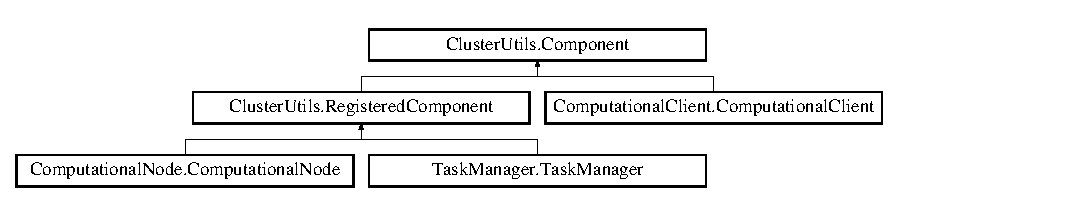
\includegraphics[height=2.276423cm]{class_cluster_utils_1_1_component}
\end{center}
\end{figure}
\subsection*{Protected Member Functions}
\begin{DoxyCompactItemize}
\item 
\hyperlink{class_cluster_utils_1_1_component_aa9235e09af855b4d29259ca086a1432f}{Component} (\hyperlink{class_cluster_utils_1_1_component_config}{Component\+Config} config, string type)
\item 
void \hyperlink{class_cluster_utils_1_1_component_a55dbb672ff63763256586cf481762dcb}{Log\+Runtime\+Info} ()
\begin{DoxyCompactList}\small\item\em Method logging components type and server info. \end{DoxyCompactList}\item 
Xml\+Document \hyperlink{class_cluster_utils_1_1_component_affb25647a4c013dee3ab2b6f82239238}{Send\+Message\+Single\+Response} (\hyperlink{interface_cluster_messages_1_1_i_cluster_message}{I\+Cluster\+Message} message)
\begin{DoxyCompactList}\small\item\em Sends single message to server and waits for single response. \end{DoxyCompactList}\item 
List$<$ Xml\+Document $>$ \hyperlink{class_cluster_utils_1_1_component_a559397a5cfeeb494a19da1bdd02f8ac0}{Send\+Message} (\hyperlink{interface_cluster_messages_1_1_i_cluster_message}{I\+Cluster\+Message} message)
\begin{DoxyCompactList}\small\item\em General method for sending messages. Sends single message to server and waits for any responses. \end{DoxyCompactList}\end{DoxyCompactItemize}
\subsection*{Protected Attributes}
\begin{DoxyCompactItemize}
\item 
\hyperlink{class_cluster_utils_1_1_server_info}{Server\+Info} \hyperlink{class_cluster_utils_1_1_component_aeeee4fbcca79664db5e301f3d5048dae}{Server\+Info}
\begin{DoxyCompactList}\small\item\em Address and port of server that this component is bound to. \end{DoxyCompactList}\item 
string \hyperlink{class_cluster_utils_1_1_component_a6ce36edcda387dbfa14f642e61f9275e}{Type}
\begin{DoxyCompactList}\small\item\em Type of component. \end{DoxyCompactList}\end{DoxyCompactItemize}


\subsection{Detailed Description}
General class for components\+: 


\begin{DoxyItemize}
\item Node
\item Manager
\item Client
\item Server as backup
\end{DoxyItemize}

Contains type and server info, and common methods for sending I\+Cluster\+Message to Server.

\subsection{Constructor \& Destructor Documentation}
\hypertarget{class_cluster_utils_1_1_component_aa9235e09af855b4d29259ca086a1432f}{}\index{Cluster\+Utils\+::\+Component@{Cluster\+Utils\+::\+Component}!Component@{Component}}
\index{Component@{Component}!Cluster\+Utils\+::\+Component@{Cluster\+Utils\+::\+Component}}
\subsubsection[{Component}]{\setlength{\rightskip}{0pt plus 5cm}Cluster\+Utils.\+Component.\+Component (
\begin{DoxyParamCaption}
\item[{{\bf Component\+Config}}]{config, }
\item[{string}]{type}
\end{DoxyParamCaption}
)\hspace{0.3cm}{\ttfamily [protected]}}\label{class_cluster_utils_1_1_component_aa9235e09af855b4d29259ca086a1432f}





\begin{DoxyParams}{Parameters}
{\em config} & Config instance containing server info.\\
\hline
{\em type} & Type of component\\
\hline
\end{DoxyParams}


\subsection{Member Function Documentation}
\hypertarget{class_cluster_utils_1_1_component_a55dbb672ff63763256586cf481762dcb}{}\index{Cluster\+Utils\+::\+Component@{Cluster\+Utils\+::\+Component}!Log\+Runtime\+Info@{Log\+Runtime\+Info}}
\index{Log\+Runtime\+Info@{Log\+Runtime\+Info}!Cluster\+Utils\+::\+Component@{Cluster\+Utils\+::\+Component}}
\subsubsection[{Log\+Runtime\+Info}]{\setlength{\rightskip}{0pt plus 5cm}void Cluster\+Utils.\+Component.\+Log\+Runtime\+Info (
\begin{DoxyParamCaption}
{}
\end{DoxyParamCaption}
)\hspace{0.3cm}{\ttfamily [protected]}}\label{class_cluster_utils_1_1_component_a55dbb672ff63763256586cf481762dcb}


Method logging components type and server info. 

\hypertarget{class_cluster_utils_1_1_component_a559397a5cfeeb494a19da1bdd02f8ac0}{}\index{Cluster\+Utils\+::\+Component@{Cluster\+Utils\+::\+Component}!Send\+Message@{Send\+Message}}
\index{Send\+Message@{Send\+Message}!Cluster\+Utils\+::\+Component@{Cluster\+Utils\+::\+Component}}
\subsubsection[{Send\+Message}]{\setlength{\rightskip}{0pt plus 5cm}List$<$Xml\+Document$>$ Cluster\+Utils.\+Component.\+Send\+Message (
\begin{DoxyParamCaption}
\item[{{\bf I\+Cluster\+Message}}]{message}
\end{DoxyParamCaption}
)\hspace{0.3cm}{\ttfamily [protected]}}\label{class_cluster_utils_1_1_component_a559397a5cfeeb494a19da1bdd02f8ac0}


General method for sending messages. Sends single message to server and waits for any responses. 


\begin{DoxyParams}{Parameters}
{\em message} & Message to be sent.\\
\hline
\end{DoxyParams}
\begin{DoxyReturn}{Returns}
All received messages as X\+M\+L\+Documents.
\end{DoxyReturn}
\hypertarget{class_cluster_utils_1_1_component_affb25647a4c013dee3ab2b6f82239238}{}\index{Cluster\+Utils\+::\+Component@{Cluster\+Utils\+::\+Component}!Send\+Message\+Single\+Response@{Send\+Message\+Single\+Response}}
\index{Send\+Message\+Single\+Response@{Send\+Message\+Single\+Response}!Cluster\+Utils\+::\+Component@{Cluster\+Utils\+::\+Component}}
\subsubsection[{Send\+Message\+Single\+Response}]{\setlength{\rightskip}{0pt plus 5cm}Xml\+Document Cluster\+Utils.\+Component.\+Send\+Message\+Single\+Response (
\begin{DoxyParamCaption}
\item[{{\bf I\+Cluster\+Message}}]{message}
\end{DoxyParamCaption}
)\hspace{0.3cm}{\ttfamily [protected]}}\label{class_cluster_utils_1_1_component_affb25647a4c013dee3ab2b6f82239238}


Sends single message to server and waits for single response. 


\begin{DoxyParams}{Parameters}
{\em message} & Message to be sent.\\
\hline
\end{DoxyParams}
\begin{DoxyReturn}{Returns}
Response from server.
\end{DoxyReturn}


\subsection{Member Data Documentation}
\hypertarget{class_cluster_utils_1_1_component_aeeee4fbcca79664db5e301f3d5048dae}{}\index{Cluster\+Utils\+::\+Component@{Cluster\+Utils\+::\+Component}!Server\+Info@{Server\+Info}}
\index{Server\+Info@{Server\+Info}!Cluster\+Utils\+::\+Component@{Cluster\+Utils\+::\+Component}}
\subsubsection[{Server\+Info}]{\setlength{\rightskip}{0pt plus 5cm}{\bf Server\+Info} Cluster\+Utils.\+Component.\+Server\+Info\hspace{0.3cm}{\ttfamily [protected]}}\label{class_cluster_utils_1_1_component_aeeee4fbcca79664db5e301f3d5048dae}


Address and port of server that this component is bound to. 

\hypertarget{class_cluster_utils_1_1_component_a6ce36edcda387dbfa14f642e61f9275e}{}\index{Cluster\+Utils\+::\+Component@{Cluster\+Utils\+::\+Component}!Type@{Type}}
\index{Type@{Type}!Cluster\+Utils\+::\+Component@{Cluster\+Utils\+::\+Component}}
\subsubsection[{Type}]{\setlength{\rightskip}{0pt plus 5cm}string Cluster\+Utils.\+Component.\+Type\hspace{0.3cm}{\ttfamily [protected]}}\label{class_cluster_utils_1_1_component_a6ce36edcda387dbfa14f642e61f9275e}


Type of component. 



The documentation for this class was generated from the following file\+:\begin{DoxyCompactItemize}
\item 
src/\+Cluster\+Utils/Component.\+cs\end{DoxyCompactItemize}

\hypertarget{class_cluster_utils_1_1_component_config}{}\section{Cluster\+Utils.\+Component\+Config Class Reference}
\label{class_cluster_utils_1_1_component_config}\index{Cluster\+Utils.\+Component\+Config@{Cluster\+Utils.\+Component\+Config}}


Container for components\textquotesingle{} configuration info -\/ server\textquotesingle{}s address and port.  


\subsection*{Static Public Member Functions}
\begin{DoxyCompactItemize}
\item 
static \hyperlink{class_cluster_utils_1_1_component_config}{Component\+Config} \hyperlink{class_cluster_utils_1_1_component_config_ae36297e732a493febbf8aa40c053adec}{Get\+Config\+From\+App\+Config} ()
\begin{DoxyCompactList}\small\item\em Retreives configuration from App.\+config file. \end{DoxyCompactList}\item 
static \hyperlink{class_cluster_utils_1_1_component_config}{Component\+Config} \hyperlink{class_cluster_utils_1_1_component_config_ac42b1e1da19f5ed827390e415e15ac0e}{Get\+Config\+From\+Args} (string\mbox{[}$\,$\mbox{]} arguments)
\begin{DoxyCompactList}\small\item\em Retreives configuration from command line arguments. \end{DoxyCompactList}\item 
static \hyperlink{class_cluster_utils_1_1_component_config}{Component\+Config} \hyperlink{class_cluster_utils_1_1_component_config_a5b2af6e5713a53c6cdaaf5da8d3231c5}{Get\+Component\+Config} (string\mbox{[}$\,$\mbox{]} arguments)
\begin{DoxyCompactList}\small\item\em Retreives config from both App.\+config and command line. Command line arguments supress App.\+config settings. \end{DoxyCompactList}\end{DoxyCompactItemize}
\subsection*{Properties}
\begin{DoxyCompactItemize}
\item 
\hypertarget{class_cluster_utils_1_1_component_config_ad0746faaef10fe71f317940febd79510}{}string {\bfseries Server\+Address}\hspace{0.3cm}{\ttfamily  \mbox{[}get, set\mbox{]}}\label{class_cluster_utils_1_1_component_config_ad0746faaef10fe71f317940febd79510}

\item 
\hypertarget{class_cluster_utils_1_1_component_config_a0479748cb87919bc45df18420b5b6395}{}string {\bfseries Server\+Port}\hspace{0.3cm}{\ttfamily  \mbox{[}get, set\mbox{]}}\label{class_cluster_utils_1_1_component_config_a0479748cb87919bc45df18420b5b6395}

\end{DoxyCompactItemize}


\subsection{Detailed Description}
Container for components\textquotesingle{} configuration info -\/ server\textquotesingle{}s address and port. 



\subsection{Member Function Documentation}
\hypertarget{class_cluster_utils_1_1_component_config_a5b2af6e5713a53c6cdaaf5da8d3231c5}{}\index{Cluster\+Utils\+::\+Component\+Config@{Cluster\+Utils\+::\+Component\+Config}!Get\+Component\+Config@{Get\+Component\+Config}}
\index{Get\+Component\+Config@{Get\+Component\+Config}!Cluster\+Utils\+::\+Component\+Config@{Cluster\+Utils\+::\+Component\+Config}}
\subsubsection[{Get\+Component\+Config}]{\setlength{\rightskip}{0pt plus 5cm}static {\bf Component\+Config} Cluster\+Utils.\+Component\+Config.\+Get\+Component\+Config (
\begin{DoxyParamCaption}
\item[{string\mbox{[}$\,$\mbox{]}}]{arguments}
\end{DoxyParamCaption}
)\hspace{0.3cm}{\ttfamily [static]}}\label{class_cluster_utils_1_1_component_config_a5b2af6e5713a53c6cdaaf5da8d3231c5}


Retreives config from both App.\+config and command line. Command line arguments supress App.\+config settings. 


\begin{DoxyParams}{Parameters}
{\em arguments} & Command line arguments.\\
\hline
\end{DoxyParams}
\begin{DoxyReturn}{Returns}
Actual component config.
\end{DoxyReturn}
\hypertarget{class_cluster_utils_1_1_component_config_ae36297e732a493febbf8aa40c053adec}{}\index{Cluster\+Utils\+::\+Component\+Config@{Cluster\+Utils\+::\+Component\+Config}!Get\+Config\+From\+App\+Config@{Get\+Config\+From\+App\+Config}}
\index{Get\+Config\+From\+App\+Config@{Get\+Config\+From\+App\+Config}!Cluster\+Utils\+::\+Component\+Config@{Cluster\+Utils\+::\+Component\+Config}}
\subsubsection[{Get\+Config\+From\+App\+Config}]{\setlength{\rightskip}{0pt plus 5cm}static {\bf Component\+Config} Cluster\+Utils.\+Component\+Config.\+Get\+Config\+From\+App\+Config (
\begin{DoxyParamCaption}
{}
\end{DoxyParamCaption}
)\hspace{0.3cm}{\ttfamily [static]}}\label{class_cluster_utils_1_1_component_config_ae36297e732a493febbf8aa40c053adec}


Retreives configuration from App.\+config file. 

\begin{DoxyReturn}{Returns}
Config from App.\+config
\end{DoxyReturn}
\hypertarget{class_cluster_utils_1_1_component_config_ac42b1e1da19f5ed827390e415e15ac0e}{}\index{Cluster\+Utils\+::\+Component\+Config@{Cluster\+Utils\+::\+Component\+Config}!Get\+Config\+From\+Args@{Get\+Config\+From\+Args}}
\index{Get\+Config\+From\+Args@{Get\+Config\+From\+Args}!Cluster\+Utils\+::\+Component\+Config@{Cluster\+Utils\+::\+Component\+Config}}
\subsubsection[{Get\+Config\+From\+Args}]{\setlength{\rightskip}{0pt plus 5cm}static {\bf Component\+Config} Cluster\+Utils.\+Component\+Config.\+Get\+Config\+From\+Args (
\begin{DoxyParamCaption}
\item[{string\mbox{[}$\,$\mbox{]}}]{arguments}
\end{DoxyParamCaption}
)\hspace{0.3cm}{\ttfamily [static]}}\label{class_cluster_utils_1_1_component_config_ac42b1e1da19f5ed827390e415e15ac0e}


Retreives configuration from command line arguments. 


\begin{DoxyParams}{Parameters}
{\em arguments} & Command line args.\\
\hline
\end{DoxyParams}
\begin{DoxyReturn}{Returns}
Config from command line args.
\end{DoxyReturn}


The documentation for this class was generated from the following file\+:\begin{DoxyCompactItemize}
\item 
src/\+Cluster\+Utils/Component\+Config.\+cs\end{DoxyCompactItemize}

\hypertarget{class_cluster_utils_tests_1_1_component_config_parser_test}{}\section{Cluster\+Utils\+Tests.\+Component\+Config\+Parser\+Test Class Reference}
\label{class_cluster_utils_tests_1_1_component_config_parser_test}\index{Cluster\+Utils\+Tests.\+Component\+Config\+Parser\+Test@{Cluster\+Utils\+Tests.\+Component\+Config\+Parser\+Test}}
\subsection*{Public Member Functions}
\begin{DoxyCompactItemize}
\item 
\hypertarget{class_cluster_utils_tests_1_1_component_config_parser_test_aa1699ad95c3b51b23c17141e0876be8b}{}void {\bfseries Check\+Config\+Availability} ()\label{class_cluster_utils_tests_1_1_component_config_parser_test_aa1699ad95c3b51b23c17141e0876be8b}

\item 
\hypertarget{class_cluster_utils_tests_1_1_component_config_parser_test_a1cc5814ea337b0cacf2c7eefa40b2782}{}void {\bfseries Override\+Server\+Address\+In\+Args} ()\label{class_cluster_utils_tests_1_1_component_config_parser_test_a1cc5814ea337b0cacf2c7eefa40b2782}

\item 
\hypertarget{class_cluster_utils_tests_1_1_component_config_parser_test_aa2b2816eac6615a82f7583e1c662b1a1}{}void {\bfseries Override\+Server\+Port\+In\+Args} ()\label{class_cluster_utils_tests_1_1_component_config_parser_test_aa2b2816eac6615a82f7583e1c662b1a1}

\end{DoxyCompactItemize}


The documentation for this class was generated from the following file\+:\begin{DoxyCompactItemize}
\item 
src/test/\+Cluster\+Utils\+Tests/Component\+Config\+Parser\+Test.\+cs\end{DoxyCompactItemize}

\hypertarget{class_communication_server_1_1_component_status}{}\section{Communication\+Server.\+Component\+Status Class Reference}
\label{class_communication_server_1_1_component_status}\index{Communication\+Server.\+Component\+Status@{Communication\+Server.\+Component\+Status}}
\subsection*{Public Member Functions}
\begin{DoxyCompactItemize}
\item 
\hypertarget{class_communication_server_1_1_component_status_ab0c457e0716d6bc55c5ff9c8eb61e78b}{}{\bfseries Component\+Status} (ulong id\+Val, String type\+Val, String\mbox{[}$\,$\mbox{]} problems\+Val)\label{class_communication_server_1_1_component_status_ab0c457e0716d6bc55c5ff9c8eb61e78b}

\end{DoxyCompactItemize}
\subsection*{Public Attributes}
\begin{DoxyCompactItemize}
\item 
\hypertarget{class_communication_server_1_1_component_status_a7954de9d1f582b032074564372415cb4}{}ulong {\bfseries id}\label{class_communication_server_1_1_component_status_a7954de9d1f582b032074564372415cb4}

\item 
\hypertarget{class_communication_server_1_1_component_status_a0e992fe6b9c40d68ecdcb1919ed881e7}{}String {\bfseries type}\label{class_communication_server_1_1_component_status_a0e992fe6b9c40d68ecdcb1919ed881e7}

\item 
\hypertarget{class_communication_server_1_1_component_status_a1577761590937eb560f1764a9f1ed62e}{}String\mbox{[}$\,$\mbox{]} {\bfseries solvable\+Problems}\label{class_communication_server_1_1_component_status_a1577761590937eb560f1764a9f1ed62e}

\end{DoxyCompactItemize}


The documentation for this class was generated from the following file\+:\begin{DoxyCompactItemize}
\item 
src/\+Communication\+Server/Component\+Status.\+cs\end{DoxyCompactItemize}

\hypertarget{class_computational_client_1_1_computational_client}{}\section{Computational\+Client.\+Computational\+Client Class Reference}
\label{class_computational_client_1_1_computational_client}\index{Computational\+Client.\+Computational\+Client@{Computational\+Client.\+Computational\+Client}}


Implementation of computational client. Allows to send single problem instance to server and repeatedly ask for final solution.  


Inheritance diagram for Computational\+Client.\+Computational\+Client\+:\begin{figure}[H]
\begin{center}
\leavevmode
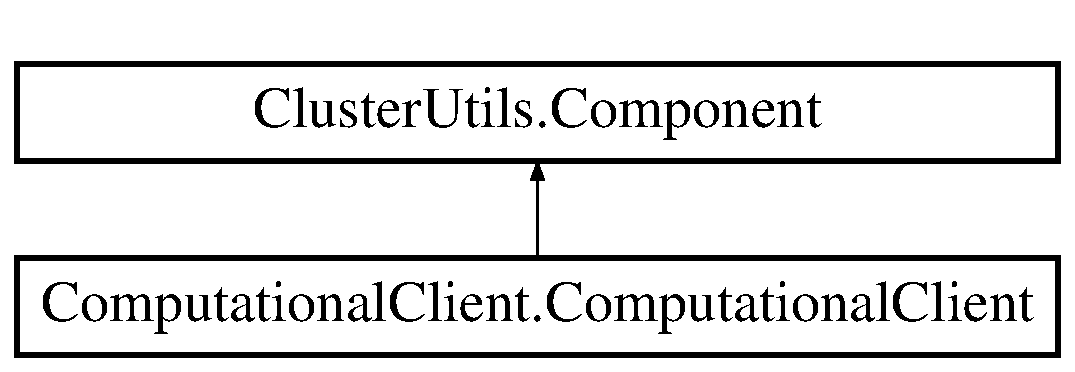
\includegraphics[height=2.000000cm]{class_computational_client_1_1_computational_client}
\end{center}
\end{figure}
\subsection*{Public Member Functions}
\begin{DoxyCompactItemize}
\item 
\hyperlink{class_computational_client_1_1_computational_client_a82b36bf9a5245a752c3b96b8947c1dc5}{Computational\+Client} (\hyperlink{class_cluster_utils_1_1_component_config}{Component\+Config} component\+Config)
\item 
void \hyperlink{class_computational_client_1_1_computational_client_abd04e67e171f547a6f112bc33c71cb79}{Start} ()
\begin{DoxyCompactList}\small\item\em Sends empty problem instance to server and starts awaiting for solution. \end{DoxyCompactList}\end{DoxyCompactItemize}
\subsection*{Additional Inherited Members}


\subsection{Detailed Description}
Implementation of computational client. Allows to send single problem instance to server and repeatedly ask for final solution. 



\subsection{Constructor \& Destructor Documentation}
\hypertarget{class_computational_client_1_1_computational_client_a82b36bf9a5245a752c3b96b8947c1dc5}{}\index{Computational\+Client\+::\+Computational\+Client@{Computational\+Client\+::\+Computational\+Client}!Computational\+Client@{Computational\+Client}}
\index{Computational\+Client@{Computational\+Client}!Computational\+Client\+::\+Computational\+Client@{Computational\+Client\+::\+Computational\+Client}}
\subsubsection[{Computational\+Client}]{\setlength{\rightskip}{0pt plus 5cm}Computational\+Client.\+Computational\+Client.\+Computational\+Client (
\begin{DoxyParamCaption}
\item[{{\bf Component\+Config}}]{component\+Config}
\end{DoxyParamCaption}
)}\label{class_computational_client_1_1_computational_client_a82b36bf9a5245a752c3b96b8947c1dc5}





\begin{DoxyParams}{Parameters}
{\em component\+Config} & Server info from App.\+config and arguments.\\
\hline
\end{DoxyParams}


\subsection{Member Function Documentation}
\hypertarget{class_computational_client_1_1_computational_client_abd04e67e171f547a6f112bc33c71cb79}{}\index{Computational\+Client\+::\+Computational\+Client@{Computational\+Client\+::\+Computational\+Client}!Start@{Start}}
\index{Start@{Start}!Computational\+Client\+::\+Computational\+Client@{Computational\+Client\+::\+Computational\+Client}}
\subsubsection[{Start}]{\setlength{\rightskip}{0pt plus 5cm}void Computational\+Client.\+Computational\+Client.\+Start (
\begin{DoxyParamCaption}
{}
\end{DoxyParamCaption}
)}\label{class_computational_client_1_1_computational_client_abd04e67e171f547a6f112bc33c71cb79}


Sends empty problem instance to server and starts awaiting for solution. 



The documentation for this class was generated from the following file\+:\begin{DoxyCompactItemize}
\item 
src/\+Computational\+Client/Computational\+Client.\+cs\end{DoxyCompactItemize}

\hypertarget{class_computational_node_1_1_computational_node}{}\section{Computational\+Node.\+Computational\+Node Class Reference}
\label{class_computational_node_1_1_computational_node}\index{Computational\+Node.\+Computational\+Node@{Computational\+Node.\+Computational\+Node}}
Inheritance diagram for Computational\+Node.\+Computational\+Node\+:\begin{figure}[H]
\begin{center}
\leavevmode
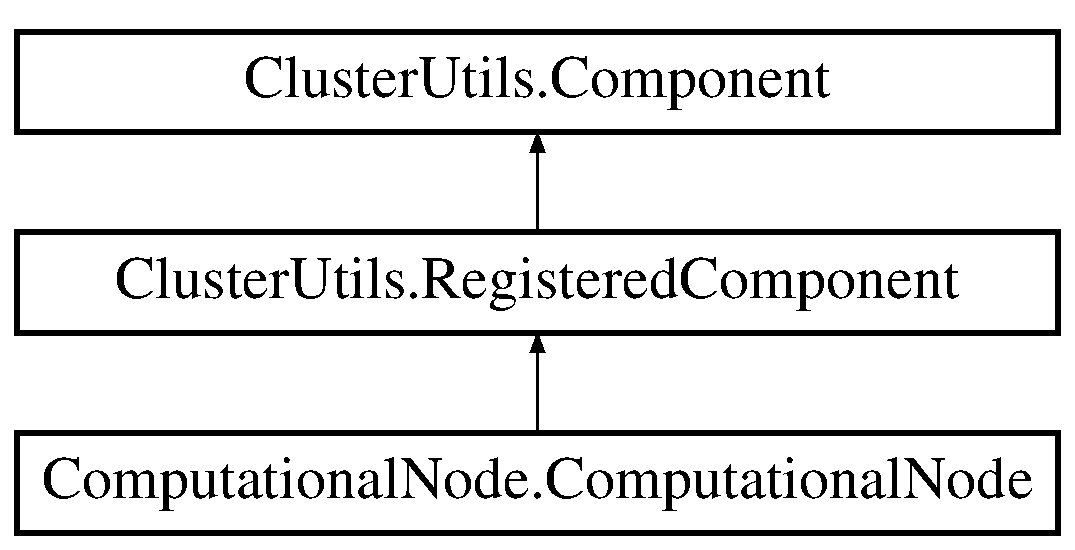
\includegraphics[height=3.000000cm]{class_computational_node_1_1_computational_node}
\end{center}
\end{figure}
\subsection*{Public Member Functions}
\begin{DoxyCompactItemize}
\item 
\hyperlink{class_computational_node_1_1_computational_node_a04b0aa3eac135d07f8886d63577bd5f0}{Computational\+Node} (\hyperlink{class_cluster_utils_1_1_component_config}{Component\+Config} component\+Config)
\item 
\hypertarget{class_computational_node_1_1_computational_node_a56a929cfb1edb87ac11242fe81048b43}{}void {\bfseries Start} ()\label{class_computational_node_1_1_computational_node_a56a929cfb1edb87ac11242fe81048b43}

\end{DoxyCompactItemize}
\subsection*{Protected Member Functions}
\begin{DoxyCompactItemize}
\item 
override void \hyperlink{class_computational_node_1_1_computational_node_ae7e1583dbbdcdc24d4b342657c4e2d5e}{Process\+Messages} (I\+Enumerable$<$ Xml\+Document $>$ responses)
\begin{DoxyCompactList}\small\item\em Method for handling all messages that given components may handle. \end{DoxyCompactList}\end{DoxyCompactItemize}
\subsection*{Additional Inherited Members}


\subsection{Constructor \& Destructor Documentation}
\hypertarget{class_computational_node_1_1_computational_node_a04b0aa3eac135d07f8886d63577bd5f0}{}\index{Computational\+Node\+::\+Computational\+Node@{Computational\+Node\+::\+Computational\+Node}!Computational\+Node@{Computational\+Node}}
\index{Computational\+Node@{Computational\+Node}!Computational\+Node\+::\+Computational\+Node@{Computational\+Node\+::\+Computational\+Node}}
\subsubsection[{Computational\+Node}]{\setlength{\rightskip}{0pt plus 5cm}Computational\+Node.\+Computational\+Node.\+Computational\+Node (
\begin{DoxyParamCaption}
\item[{{\bf Component\+Config}}]{component\+Config}
\end{DoxyParamCaption}
)}\label{class_computational_node_1_1_computational_node_a04b0aa3eac135d07f8886d63577bd5f0}





\begin{DoxyParams}{Parameters}
{\em component\+Config} & Server info from App.\+config and arguments.\\
\hline
\end{DoxyParams}


\subsection{Member Function Documentation}
\hypertarget{class_computational_node_1_1_computational_node_ae7e1583dbbdcdc24d4b342657c4e2d5e}{}\index{Computational\+Node\+::\+Computational\+Node@{Computational\+Node\+::\+Computational\+Node}!Process\+Messages@{Process\+Messages}}
\index{Process\+Messages@{Process\+Messages}!Computational\+Node\+::\+Computational\+Node@{Computational\+Node\+::\+Computational\+Node}}
\subsubsection[{Process\+Messages}]{\setlength{\rightskip}{0pt plus 5cm}override void Computational\+Node.\+Computational\+Node.\+Process\+Messages (
\begin{DoxyParamCaption}
\item[{I\+Enumerable$<$ Xml\+Document $>$}]{responses}
\end{DoxyParamCaption}
)\hspace{0.3cm}{\ttfamily [protected]}, {\ttfamily [virtual]}}\label{class_computational_node_1_1_computational_node_ae7e1583dbbdcdc24d4b342657c4e2d5e}


Method for handling all messages that given components may handle. 


\begin{DoxyParams}{Parameters}
{\em responses} & Messages received from server.\\
\hline
\end{DoxyParams}


Implements \hyperlink{class_cluster_utils_1_1_registered_component_ad5ea6fe7d138e7c6bb457c7dca203040}{Cluster\+Utils.\+Registered\+Component}.



The documentation for this class was generated from the following file\+:\begin{DoxyCompactItemize}
\item 
src/\+Computational\+Node/Computational\+Node.\+cs\end{DoxyCompactItemize}

\hypertarget{class_cluster_utils_1_1_communication_1_1_connection_client}{}\section{Cluster\+Utils.\+Communication.\+Connection\+Client Class Reference}
\label{class_cluster_utils_1_1_communication_1_1_connection_client}\index{Cluster\+Utils.\+Communication.\+Connection\+Client@{Cluster\+Utils.\+Communication.\+Connection\+Client}}


Helper class for components to communicate with server. When instance of \hyperlink{class_cluster_utils_1_1_communication_1_1_connection_client}{Connection\+Client} is created, component may open connection with server. Than component may send messages to server and wait for response/responses. Than connection is closed manually by component.  


\subsection*{Public Member Functions}
\begin{DoxyCompactItemize}
\item 
\hyperlink{class_cluster_utils_1_1_communication_1_1_connection_client_a5a9bddaca9c5264f760e8b5e51abbd44}{Connection\+Client} (\hyperlink{class_cluster_utils_1_1_server_info}{Server\+Info} server\+Info)
\item 
void \hyperlink{class_cluster_utils_1_1_communication_1_1_connection_client_a29d7584137a1f37fca15882812940899}{Connect} ()
\begin{DoxyCompactList}\small\item\em Connects client with server. \end{DoxyCompactList}\item 
List$<$ Xml\+Document $>$ \hyperlink{class_cluster_utils_1_1_communication_1_1_connection_client_a0c3e47e7c669479d4804c240bc9c87ff}{Send\+And\+Wait\+For\+Responses} (\hyperlink{interface_cluster_messages_1_1_i_cluster_message}{I\+Cluster\+Message} message)
\begin{DoxyCompactList}\small\item\em Sends message to server and waits for responses. \end{DoxyCompactList}\item 
void \hyperlink{class_cluster_utils_1_1_communication_1_1_connection_client_a6a2134ebda6076f29968e0216c25c132}{Close} ()
\begin{DoxyCompactList}\small\item\em Closes sockets between server and client. \end{DoxyCompactList}\end{DoxyCompactItemize}


\subsection{Detailed Description}
Helper class for components to communicate with server. When instance of \hyperlink{class_cluster_utils_1_1_communication_1_1_connection_client}{Connection\+Client} is created, component may open connection with server. Than component may send messages to server and wait for response/responses. Than connection is closed manually by component. 



\subsection{Constructor \& Destructor Documentation}
\hypertarget{class_cluster_utils_1_1_communication_1_1_connection_client_a5a9bddaca9c5264f760e8b5e51abbd44}{}\index{Cluster\+Utils\+::\+Communication\+::\+Connection\+Client@{Cluster\+Utils\+::\+Communication\+::\+Connection\+Client}!Connection\+Client@{Connection\+Client}}
\index{Connection\+Client@{Connection\+Client}!Cluster\+Utils\+::\+Communication\+::\+Connection\+Client@{Cluster\+Utils\+::\+Communication\+::\+Connection\+Client}}
\subsubsection[{Connection\+Client}]{\setlength{\rightskip}{0pt plus 5cm}Cluster\+Utils.\+Communication.\+Connection\+Client.\+Connection\+Client (
\begin{DoxyParamCaption}
\item[{{\bf Server\+Info}}]{server\+Info}
\end{DoxyParamCaption}
)}\label{class_cluster_utils_1_1_communication_1_1_connection_client_a5a9bddaca9c5264f760e8b5e51abbd44}





\begin{DoxyParams}{Parameters}
{\em server\+Info} & Server address and port.\\
\hline
\end{DoxyParams}


\subsection{Member Function Documentation}
\hypertarget{class_cluster_utils_1_1_communication_1_1_connection_client_a6a2134ebda6076f29968e0216c25c132}{}\index{Cluster\+Utils\+::\+Communication\+::\+Connection\+Client@{Cluster\+Utils\+::\+Communication\+::\+Connection\+Client}!Close@{Close}}
\index{Close@{Close}!Cluster\+Utils\+::\+Communication\+::\+Connection\+Client@{Cluster\+Utils\+::\+Communication\+::\+Connection\+Client}}
\subsubsection[{Close}]{\setlength{\rightskip}{0pt plus 5cm}void Cluster\+Utils.\+Communication.\+Connection\+Client.\+Close (
\begin{DoxyParamCaption}
{}
\end{DoxyParamCaption}
)}\label{class_cluster_utils_1_1_communication_1_1_connection_client_a6a2134ebda6076f29968e0216c25c132}


Closes sockets between server and client. 

\hypertarget{class_cluster_utils_1_1_communication_1_1_connection_client_a29d7584137a1f37fca15882812940899}{}\index{Cluster\+Utils\+::\+Communication\+::\+Connection\+Client@{Cluster\+Utils\+::\+Communication\+::\+Connection\+Client}!Connect@{Connect}}
\index{Connect@{Connect}!Cluster\+Utils\+::\+Communication\+::\+Connection\+Client@{Cluster\+Utils\+::\+Communication\+::\+Connection\+Client}}
\subsubsection[{Connect}]{\setlength{\rightskip}{0pt plus 5cm}void Cluster\+Utils.\+Communication.\+Connection\+Client.\+Connect (
\begin{DoxyParamCaption}
{}
\end{DoxyParamCaption}
)}\label{class_cluster_utils_1_1_communication_1_1_connection_client_a29d7584137a1f37fca15882812940899}


Connects client with server. 

\hypertarget{class_cluster_utils_1_1_communication_1_1_connection_client_a0c3e47e7c669479d4804c240bc9c87ff}{}\index{Cluster\+Utils\+::\+Communication\+::\+Connection\+Client@{Cluster\+Utils\+::\+Communication\+::\+Connection\+Client}!Send\+And\+Wait\+For\+Responses@{Send\+And\+Wait\+For\+Responses}}
\index{Send\+And\+Wait\+For\+Responses@{Send\+And\+Wait\+For\+Responses}!Cluster\+Utils\+::\+Communication\+::\+Connection\+Client@{Cluster\+Utils\+::\+Communication\+::\+Connection\+Client}}
\subsubsection[{Send\+And\+Wait\+For\+Responses}]{\setlength{\rightskip}{0pt plus 5cm}List$<$Xml\+Document$>$ Cluster\+Utils.\+Communication.\+Connection\+Client.\+Send\+And\+Wait\+For\+Responses (
\begin{DoxyParamCaption}
\item[{{\bf I\+Cluster\+Message}}]{message}
\end{DoxyParamCaption}
)}\label{class_cluster_utils_1_1_communication_1_1_connection_client_a0c3e47e7c669479d4804c240bc9c87ff}


Sends message to server and waits for responses. 


\begin{DoxyParams}{Parameters}
{\em message} & Message to be sent.\\
\hline
\end{DoxyParams}
\begin{DoxyReturn}{Returns}
All possible responses.
\end{DoxyReturn}


The documentation for this class was generated from the following file\+:\begin{DoxyCompactItemize}
\item 
src/\+Cluster\+Utils/\+Communication/Connection\+Client.\+cs\end{DoxyCompactItemize}

\hypertarget{class_divide_problem}{}\section{Divide\+Problem Class Reference}
\label{class_divide_problem}\index{Divide\+Problem@{Divide\+Problem}}


$<$uwagi$>$  


Inheritance diagram for Divide\+Problem\+:\begin{figure}[H]
\begin{center}
\leavevmode
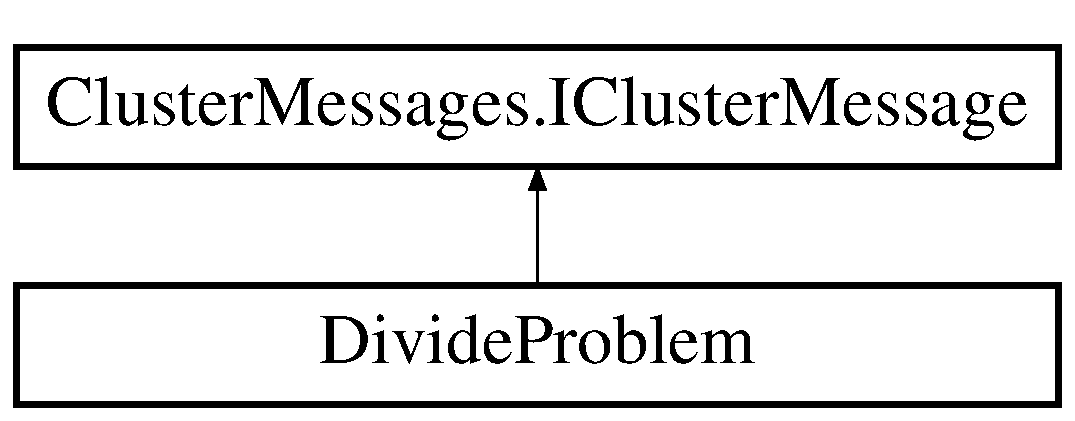
\includegraphics[height=2.000000cm]{class_divide_problem}
\end{center}
\end{figure}
\subsection*{Properties}
\begin{DoxyCompactItemize}
\item 
\hypertarget{class_divide_problem_a454c1db897dfce75326566677e77a396}{}string \hyperlink{class_divide_problem_a454c1db897dfce75326566677e77a396}{Problem\+Type}\hspace{0.3cm}{\ttfamily  \mbox{[}get, set\mbox{]}}\label{class_divide_problem_a454c1db897dfce75326566677e77a396}

\begin{DoxyCompactList}\small\item\em $<$uwagi$>$ \end{DoxyCompactList}\item 
\hypertarget{class_divide_problem_af5b70cb0ae5f7e53c7d2b40de4afa40b}{}ulong \hyperlink{class_divide_problem_af5b70cb0ae5f7e53c7d2b40de4afa40b}{Id}\hspace{0.3cm}{\ttfamily  \mbox{[}get, set\mbox{]}}\label{class_divide_problem_af5b70cb0ae5f7e53c7d2b40de4afa40b}

\begin{DoxyCompactList}\small\item\em $<$uwagi$>$ \end{DoxyCompactList}\item 
\hypertarget{class_divide_problem_ae0a6a0f1980fb4d7fac621d79d9b24fc}{}byte\mbox{[}$\,$\mbox{]} \hyperlink{class_divide_problem_ae0a6a0f1980fb4d7fac621d79d9b24fc}{Data}\hspace{0.3cm}{\ttfamily  \mbox{[}get, set\mbox{]}}\label{class_divide_problem_ae0a6a0f1980fb4d7fac621d79d9b24fc}

\begin{DoxyCompactList}\small\item\em $<$uwagi$>$ \end{DoxyCompactList}\item 
\hypertarget{class_divide_problem_ae191e52a3d606453d75b9346dc0af7c1}{}ulong \hyperlink{class_divide_problem_ae191e52a3d606453d75b9346dc0af7c1}{Computational\+Nodes}\hspace{0.3cm}{\ttfamily  \mbox{[}get, set\mbox{]}}\label{class_divide_problem_ae191e52a3d606453d75b9346dc0af7c1}

\begin{DoxyCompactList}\small\item\em $<$uwagi$>$ \end{DoxyCompactList}\item 
\hypertarget{class_divide_problem_ac60e4cc3173e4d9493ecba6d5e001e54}{}ulong \hyperlink{class_divide_problem_ac60e4cc3173e4d9493ecba6d5e001e54}{Node\+I\+D}\hspace{0.3cm}{\ttfamily  \mbox{[}get, set\mbox{]}}\label{class_divide_problem_ac60e4cc3173e4d9493ecba6d5e001e54}

\begin{DoxyCompactList}\small\item\em $<$uwagi$>$ \end{DoxyCompactList}\end{DoxyCompactItemize}


\subsection{Detailed Description}
$<$uwagi$>$ 

The documentation for this class was generated from the following file\+:\begin{DoxyCompactItemize}
\item 
src/\+Cluster\+Messages/\+Generated\+Messages/Divide\+Problem.\+cs\end{DoxyCompactItemize}

\hypertarget{interface_cluster_messages_1_1_i_cluster_message}{}\section{Cluster\+Messages.\+I\+Cluster\+Message Interface Reference}
\label{interface_cluster_messages_1_1_i_cluster_message}\index{Cluster\+Messages.\+I\+Cluster\+Message@{Cluster\+Messages.\+I\+Cluster\+Message}}


General interface for message classes generated from Xml Schemas.  


Inheritance diagram for Cluster\+Messages.\+I\+Cluster\+Message\+:\begin{figure}[H]
\begin{center}
\leavevmode
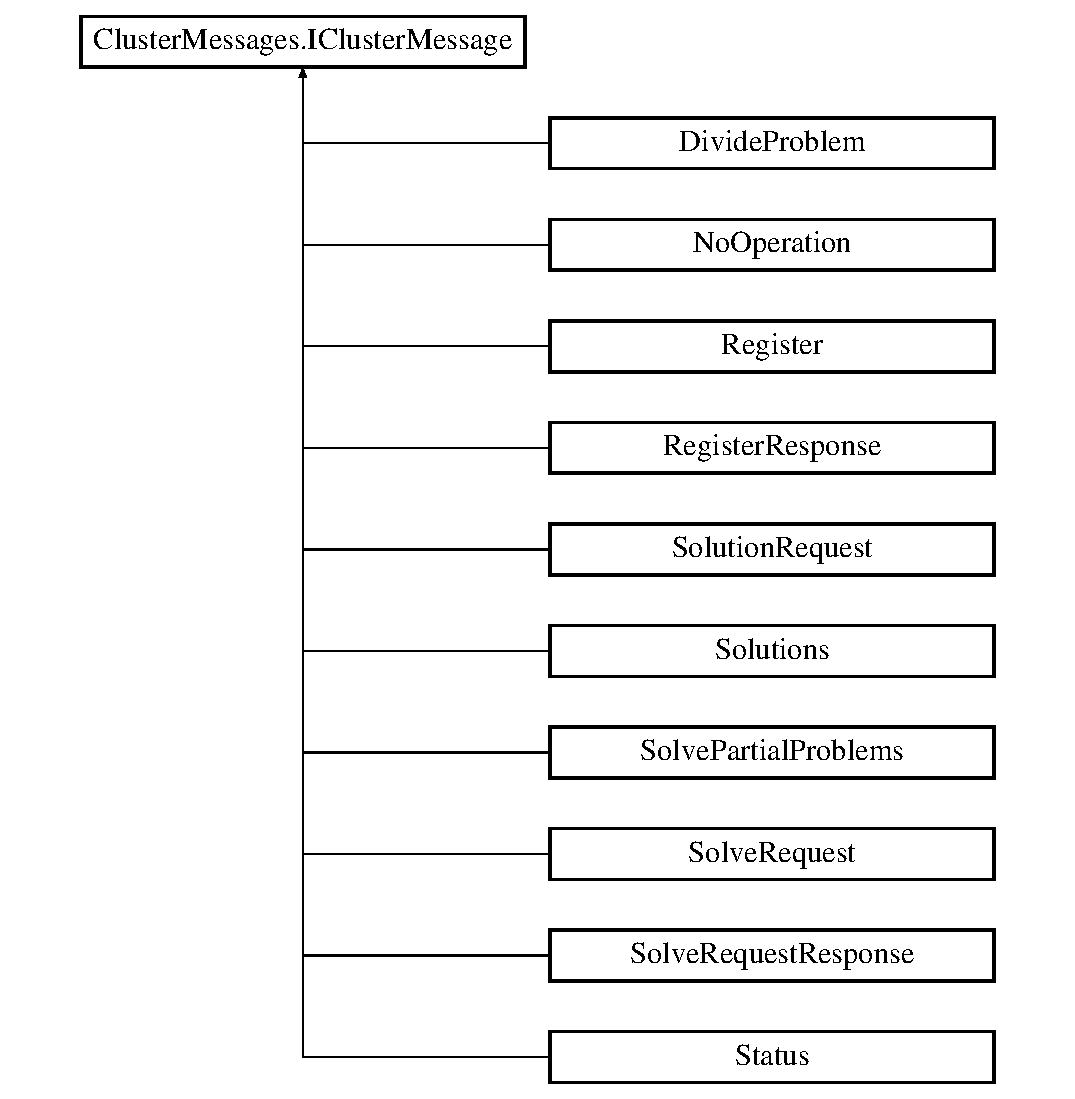
\includegraphics[height=11.000000cm]{interface_cluster_messages_1_1_i_cluster_message}
\end{center}
\end{figure}


\subsection{Detailed Description}
General interface for message classes generated from Xml Schemas. 



The documentation for this interface was generated from the following file\+:\begin{DoxyCompactItemize}
\item 
src/\+Cluster\+Messages/Cluster\+Message.\+cs\end{DoxyCompactItemize}

\hypertarget{class_communication_server_1_1_message_dispatcher}{}\section{Communication\+Server.\+Message\+Dispatcher Class Reference}
\label{class_communication_server_1_1_message_dispatcher}\index{Communication\+Server.\+Message\+Dispatcher@{Communication\+Server.\+Message\+Dispatcher}}
\subsection*{Public Member Functions}
\begin{DoxyCompactItemize}
\item 
\hypertarget{class_communication_server_1_1_message_dispatcher_a4b2daf0a094e8477712b1fce3f6051f3}{}{\bfseries Message\+Dispatcher} (string listport, int timeout)\label{class_communication_server_1_1_message_dispatcher_a4b2daf0a094e8477712b1fce3f6051f3}

\item 
void \hyperlink{class_communication_server_1_1_message_dispatcher_ab853c64f7c38ee8b4afbd0f02dbf4c49}{Begin\+Dispatching} ()
\begin{DoxyCompactList}\small\item\em Starts listening thread \end{DoxyCompactList}\item 
void \hyperlink{class_communication_server_1_1_message_dispatcher_a638aa74e23ab23176a4e23890e6beeb4}{Listening\+Thread} (Object o)
\begin{DoxyCompactList}\small\item\em Listens for messages from other components \end{DoxyCompactList}\item 
\hypertarget{class_communication_server_1_1_message_dispatcher_a1b3d608182a9dc9a5c4faaced34bc104}{}void {\bfseries Message\+Read\+Thread} (Object obj)\label{class_communication_server_1_1_message_dispatcher_a1b3d608182a9dc9a5c4faaced34bc104}

\item 
void \hyperlink{class_communication_server_1_1_message_dispatcher_a52e2c5b8822535187f3b0bffcb591e55}{Analyze\+Message} (\hyperlink{class_communication_server_1_1_thread_package}{Thread\+Package} tp)
\begin{DoxyCompactList}\small\item\em Analyzes different messages types \end{DoxyCompactList}\item 
void \hyperlink{class_communication_server_1_1_message_dispatcher_a6b9ce154fa93df43deafb14853deda65}{Handle\+State\+Messages} (\hyperlink{class_communication_server_1_1_thread_package}{Thread\+Package} tp)
\begin{DoxyCompactList}\small\item\em Handles State Messages from components \end{DoxyCompactList}\item 
void \hyperlink{class_communication_server_1_1_message_dispatcher_a95026cfe10919dc54b5e7c36fd914ac8}{Handle\+Register\+Messages} (\hyperlink{class_communication_server_1_1_thread_package}{Thread\+Package} tp)
\begin{DoxyCompactList}\small\item\em Handles \hyperlink{class_register}{Register} Messages from components \end{DoxyCompactList}\item 
void \hyperlink{class_communication_server_1_1_message_dispatcher_aa6b578088c880c0e53350a4a4f6eb885}{Handle\+Solve\+Request\+Messages} (\hyperlink{class_communication_server_1_1_thread_package}{Thread\+Package} tp)
\begin{DoxyCompactList}\small\item\em Handles \hyperlink{class_solve_request}{Solve\+Request} Messages from Client \end{DoxyCompactList}\item 
void \hyperlink{class_communication_server_1_1_message_dispatcher_aaa48feaa1ebb84f174cd5a750a3d63a6}{Handle\+Solution\+Request\+Messages} (\hyperlink{class_communication_server_1_1_thread_package}{Thread\+Package} tp)
\begin{DoxyCompactList}\small\item\em Handles \hyperlink{class_solution_request}{Solution\+Request} Messages from Client \end{DoxyCompactList}\item 
void \hyperlink{class_communication_server_1_1_message_dispatcher_ac49238ac7a476766ba98a653d4ed3871}{Handle\+Partial\+Problems\+Messages} (\hyperlink{class_communication_server_1_1_thread_package}{Thread\+Package} tp)
\begin{DoxyCompactList}\small\item\em Handles Solve\+Partial\+Problem Messages from components and sends \hyperlink{class_no_operation}{No\+Operation} response \end{DoxyCompactList}\item 
void \hyperlink{class_communication_server_1_1_message_dispatcher_a8f18f2d10e25186d1880c1d3bc2f2310}{Handle\+Solution\+Messages} (\hyperlink{class_communication_server_1_1_thread_package}{Thread\+Package} tp)
\begin{DoxyCompactList}\small\item\em Handles Solution Messages from components and sends \hyperlink{class_no_operation}{No\+Operation} response. If Solution is Final, prepares it to send it to Client. If Solution is Partial, adds it to the \+\_\+partial\+Solutions list \end{DoxyCompactList}\item 
void \hyperlink{class_communication_server_1_1_message_dispatcher_a0a7ba1a0e7cc4ad3cad9c8667783b3a1}{Handle\+Final\+Solution\+Messages} (\hyperlink{class_communication_server_1_1_thread_package}{Thread\+Package} tp)
\begin{DoxyCompactList}\small\item\em Handles Partial \hyperlink{class_solutions}{Solutions} Messages from components \end{DoxyCompactList}\item 
void \hyperlink{class_communication_server_1_1_message_dispatcher_a89db15326a47cc13771a5108640cc231}{Handle\+Partial\+Solution\+Messages} (\hyperlink{class_communication_server_1_1_thread_package}{Thread\+Package} tp)
\begin{DoxyCompactList}\small\item\em Handles Final Solution from components \end{DoxyCompactList}\item 
void \hyperlink{class_communication_server_1_1_message_dispatcher_afe7a90c6cf0a72550a2187f6c8e14f63}{Convert\+And\+Send\+Two\+Messages$<$ T, T\+S $>$} (T message1, T\+S message2, Socket handler)
\begin{DoxyCompactList}\small\item\em Converts two Messages of different types to the binary array data and sends them to component \end{DoxyCompactList}\item 
void \hyperlink{class_communication_server_1_1_message_dispatcher_afbb0bdc3da4c4f28575bea83dbbdfdcd}{Convert\+And\+Send\+Message$<$ T $>$} (T message, Socket handler)
\begin{DoxyCompactList}\small\item\em Converts a message to binary array data and sends it to component \end{DoxyCompactList}\item 
void \hyperlink{class_communication_server_1_1_message_dispatcher_a67a6a73f07f09f0fd7a3c081d58f034f}{Send\+No\+Operation\+Message} (\hyperlink{class_communication_server_1_1_thread_package}{Thread\+Package} tp)
\begin{DoxyCompactList}\small\item\em Send \hyperlink{class_no_operation}{No\+Operation} message to component \end{DoxyCompactList}\item 
String\mbox{[}$\,$\mbox{]} \hyperlink{class_communication_server_1_1_message_dispatcher_af80a513cfca1d67a3f255a1f66cc8da2}{Create\+Array\+From\+Xml} (Xml\+Node\+List xml\+Elements\+List)
\begin{DoxyCompactList}\small\item\em Creates String array from Xml\+Node\+List element \end{DoxyCompactList}\item 
String \hyperlink{class_communication_server_1_1_message_dispatcher_aaa3c65b929c052b2f7c12ff959e38b59}{Get\+Xml\+Element\+Inner\+Text} (String s, Xml\+Document doc)
\begin{DoxyCompactList}\small\item\em Finds text value of the element in the Xml\+Document \end{DoxyCompactList}\item 
ulong \hyperlink{class_communication_server_1_1_message_dispatcher_a9faadcb5411cd281c7d0c7e9e0ad547a}{Get\+Xml\+Element\+Inner\+Ulong} (String s, Xml\+Document doc)
\begin{DoxyCompactList}\small\item\em Finds ulong value of the element in the Xml\+Document \end{DoxyCompactList}\item 
byte\mbox{[}$\,$\mbox{]} \hyperlink{class_communication_server_1_1_message_dispatcher_a837b62b4f47be46c9f1a4ae3e8866820}{Get\+Xml\+Element\+Inner\+Byte} (String s, Xml\+Document doc)
\begin{DoxyCompactList}\small\item\em Finds byte\mbox{[}\mbox{]} value of the element in the Xml\+Document \end{DoxyCompactList}\item 
void \hyperlink{class_communication_server_1_1_message_dispatcher_a918d6101f88cf8116d6b919b7923bcba}{Add\+Partial\+Solution} (\hyperlink{class_solutions_solution}{Solutions\+Solution} ss, ulong list\+Id)
\begin{DoxyCompactList}\small\item\em Adds Parital Solution to the \+\_\+partial\+Solutions list \end{DoxyCompactList}\item 
\hyperlink{interface_cluster_messages_1_1_i_cluster_message}{I\+Cluster\+Message} \hyperlink{class_communication_server_1_1_message_dispatcher_a20aa92ccb3e90d39e4b659e266004c3c}{Search\+Task\+Manager\+Messages} (ulong id, Socket handler)
\begin{DoxyCompactList}\small\item\em Searches listed messages (\hyperlink{class_solve_request}{Solve\+Request} and \hyperlink{class_solutions}{Solutions}) for \hyperlink{namespace_task_manager}{Task\+Manager} \end{DoxyCompactList}\item 
\hyperlink{interface_cluster_messages_1_1_i_cluster_message}{I\+Cluster\+Message} \hyperlink{class_communication_server_1_1_message_dispatcher_a2164a41ee186aa26fe730826a933ce9b}{Search\+Computational\+Node\+Messages} (Socket handler)
\begin{DoxyCompactList}\small\item\em Searches listed messages (\hyperlink{class_solve_partial_problems}{Solve\+Partial\+Problems}) for \hyperlink{namespace_computational_node}{Computational\+Node} \end{DoxyCompactList}\item 
\hypertarget{class_communication_server_1_1_message_dispatcher_a84feec90f6d26c683cdef194dc6d1ab6}{}void {\bfseries Accept\+Callback} (I\+Async\+Result ar)\label{class_communication_server_1_1_message_dispatcher_a84feec90f6d26c683cdef194dc6d1ab6}

\item 
\hypertarget{class_communication_server_1_1_message_dispatcher_a76d857e8279155a0aeb7790f369ebaef}{}void {\bfseries Read\+Callback} (I\+Async\+Result ar)\label{class_communication_server_1_1_message_dispatcher_a76d857e8279155a0aeb7790f369ebaef}

\end{DoxyCompactItemize}
\subsection*{Static Public Member Functions}
\begin{DoxyCompactItemize}
\item 
\hypertarget{class_communication_server_1_1_message_dispatcher_a2a513401c100e0ce8d4bc658408137d0}{}static void {\bfseries Send\+Message} (Socket handler, byte\mbox{[}$\,$\mbox{]} byte\+Data)\label{class_communication_server_1_1_message_dispatcher_a2a513401c100e0ce8d4bc658408137d0}

\end{DoxyCompactItemize}
\subsection*{Static Public Attributes}
\begin{DoxyCompactItemize}
\item 
\hypertarget{class_communication_server_1_1_message_dispatcher_a21a0b49ae2e477072964ae83645dff35}{}static Manual\+Reset\+Event {\bfseries All\+Done} = new Manual\+Reset\+Event(false)\label{class_communication_server_1_1_message_dispatcher_a21a0b49ae2e477072964ae83645dff35}

\end{DoxyCompactItemize}


\subsection{Member Function Documentation}
\hypertarget{class_communication_server_1_1_message_dispatcher_a918d6101f88cf8116d6b919b7923bcba}{}\index{Communication\+Server\+::\+Message\+Dispatcher@{Communication\+Server\+::\+Message\+Dispatcher}!Add\+Partial\+Solution@{Add\+Partial\+Solution}}
\index{Add\+Partial\+Solution@{Add\+Partial\+Solution}!Communication\+Server\+::\+Message\+Dispatcher@{Communication\+Server\+::\+Message\+Dispatcher}}
\subsubsection[{Add\+Partial\+Solution}]{\setlength{\rightskip}{0pt plus 5cm}void Communication\+Server.\+Message\+Dispatcher.\+Add\+Partial\+Solution (
\begin{DoxyParamCaption}
\item[{{\bf Solutions\+Solution}}]{ss, }
\item[{ulong}]{list\+Id}
\end{DoxyParamCaption}
)}\label{class_communication_server_1_1_message_dispatcher_a918d6101f88cf8116d6b919b7923bcba}


Adds Parital Solution to the \+\_\+partial\+Solutions list 


\begin{DoxyParams}{Parameters}
{\em ss} & Partial\+Solution that is added to the list\\
\hline
{\em list\+Id} & I\+D of \+\_\+partial\+Solutions list\\
\hline
\end{DoxyParams}
\hypertarget{class_communication_server_1_1_message_dispatcher_a52e2c5b8822535187f3b0bffcb591e55}{}\index{Communication\+Server\+::\+Message\+Dispatcher@{Communication\+Server\+::\+Message\+Dispatcher}!Analyze\+Message@{Analyze\+Message}}
\index{Analyze\+Message@{Analyze\+Message}!Communication\+Server\+::\+Message\+Dispatcher@{Communication\+Server\+::\+Message\+Dispatcher}}
\subsubsection[{Analyze\+Message}]{\setlength{\rightskip}{0pt plus 5cm}void Communication\+Server.\+Message\+Dispatcher.\+Analyze\+Message (
\begin{DoxyParamCaption}
\item[{{\bf Thread\+Package}}]{tp}
\end{DoxyParamCaption}
)}\label{class_communication_server_1_1_message_dispatcher_a52e2c5b8822535187f3b0bffcb591e55}


Analyzes different messages types 


\begin{DoxyParams}{Parameters}
{\em tp} & Thread Package with Socket handler and Xml\+Document message\\
\hline
\end{DoxyParams}
\hypertarget{class_communication_server_1_1_message_dispatcher_ab853c64f7c38ee8b4afbd0f02dbf4c49}{}\index{Communication\+Server\+::\+Message\+Dispatcher@{Communication\+Server\+::\+Message\+Dispatcher}!Begin\+Dispatching@{Begin\+Dispatching}}
\index{Begin\+Dispatching@{Begin\+Dispatching}!Communication\+Server\+::\+Message\+Dispatcher@{Communication\+Server\+::\+Message\+Dispatcher}}
\subsubsection[{Begin\+Dispatching}]{\setlength{\rightskip}{0pt plus 5cm}void Communication\+Server.\+Message\+Dispatcher.\+Begin\+Dispatching (
\begin{DoxyParamCaption}
{}
\end{DoxyParamCaption}
)}\label{class_communication_server_1_1_message_dispatcher_ab853c64f7c38ee8b4afbd0f02dbf4c49}


Starts listening thread 

\hypertarget{class_communication_server_1_1_message_dispatcher_afbb0bdc3da4c4f28575bea83dbbdfdcd}{}\index{Communication\+Server\+::\+Message\+Dispatcher@{Communication\+Server\+::\+Message\+Dispatcher}!Convert\+And\+Send\+Message$<$ T $>$@{Convert\+And\+Send\+Message$<$ T $>$}}
\index{Convert\+And\+Send\+Message$<$ T $>$@{Convert\+And\+Send\+Message$<$ T $>$}!Communication\+Server\+::\+Message\+Dispatcher@{Communication\+Server\+::\+Message\+Dispatcher}}
\subsubsection[{Convert\+And\+Send\+Message$<$ T $>$}]{\setlength{\rightskip}{0pt plus 5cm}void Communication\+Server.\+Message\+Dispatcher.\+Convert\+And\+Send\+Message$<$ T $>$ (
\begin{DoxyParamCaption}
\item[{T}]{message, }
\item[{Socket}]{handler}
\end{DoxyParamCaption}
)}\label{class_communication_server_1_1_message_dispatcher_afbb0bdc3da4c4f28575bea83dbbdfdcd}


Converts a message to binary array data and sends it to component 


\begin{DoxyTemplParams}{Template Parameters}
{\em T} & Type of the message\\
\hline
\end{DoxyTemplParams}

\begin{DoxyParams}{Parameters}
{\em message} & Message\\
\hline
{\em handler} & Socket handler of the component, that message will be sent to\\
\hline
\end{DoxyParams}
\hypertarget{class_communication_server_1_1_message_dispatcher_afe7a90c6cf0a72550a2187f6c8e14f63}{}\index{Communication\+Server\+::\+Message\+Dispatcher@{Communication\+Server\+::\+Message\+Dispatcher}!Convert\+And\+Send\+Two\+Messages$<$ T, T\+S $>$@{Convert\+And\+Send\+Two\+Messages$<$ T, T\+S $>$}}
\index{Convert\+And\+Send\+Two\+Messages$<$ T, T\+S $>$@{Convert\+And\+Send\+Two\+Messages$<$ T, T\+S $>$}!Communication\+Server\+::\+Message\+Dispatcher@{Communication\+Server\+::\+Message\+Dispatcher}}
\subsubsection[{Convert\+And\+Send\+Two\+Messages$<$ T, T\+S $>$}]{\setlength{\rightskip}{0pt plus 5cm}void Communication\+Server.\+Message\+Dispatcher.\+Convert\+And\+Send\+Two\+Messages$<$ T, T\+S $>$ (
\begin{DoxyParamCaption}
\item[{T}]{message1, }
\item[{T\+S}]{message2, }
\item[{Socket}]{handler}
\end{DoxyParamCaption}
)}\label{class_communication_server_1_1_message_dispatcher_afe7a90c6cf0a72550a2187f6c8e14f63}


Converts two Messages of different types to the binary array data and sends them to component 


\begin{DoxyTemplParams}{Template Parameters}
{\em T} & Type of the first message\\
\hline
{\em T\+S} & Type of the second message\\
\hline
\end{DoxyTemplParams}

\begin{DoxyParams}{Parameters}
{\em message1} & First message\\
\hline
{\em message2} & Second message\\
\hline
{\em handler} & Socket handler of the component, that messages will be sent to\\
\hline
\end{DoxyParams}
\hypertarget{class_communication_server_1_1_message_dispatcher_af80a513cfca1d67a3f255a1f66cc8da2}{}\index{Communication\+Server\+::\+Message\+Dispatcher@{Communication\+Server\+::\+Message\+Dispatcher}!Create\+Array\+From\+Xml@{Create\+Array\+From\+Xml}}
\index{Create\+Array\+From\+Xml@{Create\+Array\+From\+Xml}!Communication\+Server\+::\+Message\+Dispatcher@{Communication\+Server\+::\+Message\+Dispatcher}}
\subsubsection[{Create\+Array\+From\+Xml}]{\setlength{\rightskip}{0pt plus 5cm}String \mbox{[}$\,$\mbox{]} Communication\+Server.\+Message\+Dispatcher.\+Create\+Array\+From\+Xml (
\begin{DoxyParamCaption}
\item[{Xml\+Node\+List}]{xml\+Elements\+List}
\end{DoxyParamCaption}
)}\label{class_communication_server_1_1_message_dispatcher_af80a513cfca1d67a3f255a1f66cc8da2}


Creates String array from Xml\+Node\+List element 


\begin{DoxyParams}{Parameters}
{\em xml\+Elements\+List} & Xml\+Node\+List element\\
\hline
\end{DoxyParams}
\begin{DoxyReturn}{Returns}

\end{DoxyReturn}
\hypertarget{class_communication_server_1_1_message_dispatcher_a837b62b4f47be46c9f1a4ae3e8866820}{}\index{Communication\+Server\+::\+Message\+Dispatcher@{Communication\+Server\+::\+Message\+Dispatcher}!Get\+Xml\+Element\+Inner\+Byte@{Get\+Xml\+Element\+Inner\+Byte}}
\index{Get\+Xml\+Element\+Inner\+Byte@{Get\+Xml\+Element\+Inner\+Byte}!Communication\+Server\+::\+Message\+Dispatcher@{Communication\+Server\+::\+Message\+Dispatcher}}
\subsubsection[{Get\+Xml\+Element\+Inner\+Byte}]{\setlength{\rightskip}{0pt plus 5cm}byte \mbox{[}$\,$\mbox{]} Communication\+Server.\+Message\+Dispatcher.\+Get\+Xml\+Element\+Inner\+Byte (
\begin{DoxyParamCaption}
\item[{String}]{s, }
\item[{Xml\+Document}]{doc}
\end{DoxyParamCaption}
)}\label{class_communication_server_1_1_message_dispatcher_a837b62b4f47be46c9f1a4ae3e8866820}


Finds byte\mbox{[}\mbox{]} value of the element in the Xml\+Document 


\begin{DoxyParams}{Parameters}
{\em s} & Name of the element\\
\hline
{\em doc} & Xml\+Document we are searching in\\
\hline
\end{DoxyParams}
\begin{DoxyReturn}{Returns}

\end{DoxyReturn}
\hypertarget{class_communication_server_1_1_message_dispatcher_aaa3c65b929c052b2f7c12ff959e38b59}{}\index{Communication\+Server\+::\+Message\+Dispatcher@{Communication\+Server\+::\+Message\+Dispatcher}!Get\+Xml\+Element\+Inner\+Text@{Get\+Xml\+Element\+Inner\+Text}}
\index{Get\+Xml\+Element\+Inner\+Text@{Get\+Xml\+Element\+Inner\+Text}!Communication\+Server\+::\+Message\+Dispatcher@{Communication\+Server\+::\+Message\+Dispatcher}}
\subsubsection[{Get\+Xml\+Element\+Inner\+Text}]{\setlength{\rightskip}{0pt plus 5cm}String Communication\+Server.\+Message\+Dispatcher.\+Get\+Xml\+Element\+Inner\+Text (
\begin{DoxyParamCaption}
\item[{String}]{s, }
\item[{Xml\+Document}]{doc}
\end{DoxyParamCaption}
)}\label{class_communication_server_1_1_message_dispatcher_aaa3c65b929c052b2f7c12ff959e38b59}


Finds text value of the element in the Xml\+Document 


\begin{DoxyParams}{Parameters}
{\em s} & Name of the element\\
\hline
{\em doc} & Xml\+Document we are searching in\\
\hline
\end{DoxyParams}
\begin{DoxyReturn}{Returns}

\end{DoxyReturn}
\hypertarget{class_communication_server_1_1_message_dispatcher_a9faadcb5411cd281c7d0c7e9e0ad547a}{}\index{Communication\+Server\+::\+Message\+Dispatcher@{Communication\+Server\+::\+Message\+Dispatcher}!Get\+Xml\+Element\+Inner\+Ulong@{Get\+Xml\+Element\+Inner\+Ulong}}
\index{Get\+Xml\+Element\+Inner\+Ulong@{Get\+Xml\+Element\+Inner\+Ulong}!Communication\+Server\+::\+Message\+Dispatcher@{Communication\+Server\+::\+Message\+Dispatcher}}
\subsubsection[{Get\+Xml\+Element\+Inner\+Ulong}]{\setlength{\rightskip}{0pt plus 5cm}ulong Communication\+Server.\+Message\+Dispatcher.\+Get\+Xml\+Element\+Inner\+Ulong (
\begin{DoxyParamCaption}
\item[{String}]{s, }
\item[{Xml\+Document}]{doc}
\end{DoxyParamCaption}
)}\label{class_communication_server_1_1_message_dispatcher_a9faadcb5411cd281c7d0c7e9e0ad547a}


Finds ulong value of the element in the Xml\+Document 


\begin{DoxyParams}{Parameters}
{\em s} & Name of the element\\
\hline
{\em doc} & Xml\+Document we are searching in\\
\hline
\end{DoxyParams}
\begin{DoxyReturn}{Returns}

\end{DoxyReturn}
\hypertarget{class_communication_server_1_1_message_dispatcher_a0a7ba1a0e7cc4ad3cad9c8667783b3a1}{}\index{Communication\+Server\+::\+Message\+Dispatcher@{Communication\+Server\+::\+Message\+Dispatcher}!Handle\+Final\+Solution\+Messages@{Handle\+Final\+Solution\+Messages}}
\index{Handle\+Final\+Solution\+Messages@{Handle\+Final\+Solution\+Messages}!Communication\+Server\+::\+Message\+Dispatcher@{Communication\+Server\+::\+Message\+Dispatcher}}
\subsubsection[{Handle\+Final\+Solution\+Messages}]{\setlength{\rightskip}{0pt plus 5cm}void Communication\+Server.\+Message\+Dispatcher.\+Handle\+Final\+Solution\+Messages (
\begin{DoxyParamCaption}
\item[{{\bf Thread\+Package}}]{tp}
\end{DoxyParamCaption}
)}\label{class_communication_server_1_1_message_dispatcher_a0a7ba1a0e7cc4ad3cad9c8667783b3a1}


Handles Partial \hyperlink{class_solutions}{Solutions} Messages from components 


\begin{DoxyParams}{Parameters}
{\em tp} & Thread Package with Socket handler and Xml\+Document message\\
\hline
\end{DoxyParams}
\hypertarget{class_communication_server_1_1_message_dispatcher_ac49238ac7a476766ba98a653d4ed3871}{}\index{Communication\+Server\+::\+Message\+Dispatcher@{Communication\+Server\+::\+Message\+Dispatcher}!Handle\+Partial\+Problems\+Messages@{Handle\+Partial\+Problems\+Messages}}
\index{Handle\+Partial\+Problems\+Messages@{Handle\+Partial\+Problems\+Messages}!Communication\+Server\+::\+Message\+Dispatcher@{Communication\+Server\+::\+Message\+Dispatcher}}
\subsubsection[{Handle\+Partial\+Problems\+Messages}]{\setlength{\rightskip}{0pt plus 5cm}void Communication\+Server.\+Message\+Dispatcher.\+Handle\+Partial\+Problems\+Messages (
\begin{DoxyParamCaption}
\item[{{\bf Thread\+Package}}]{tp}
\end{DoxyParamCaption}
)}\label{class_communication_server_1_1_message_dispatcher_ac49238ac7a476766ba98a653d4ed3871}


Handles Solve\+Partial\+Problem Messages from components and sends \hyperlink{class_no_operation}{No\+Operation} response 


\begin{DoxyParams}{Parameters}
{\em tp} & Thread Package with Socket handler and Xml\+Document message\\
\hline
\end{DoxyParams}
\hypertarget{class_communication_server_1_1_message_dispatcher_a89db15326a47cc13771a5108640cc231}{}\index{Communication\+Server\+::\+Message\+Dispatcher@{Communication\+Server\+::\+Message\+Dispatcher}!Handle\+Partial\+Solution\+Messages@{Handle\+Partial\+Solution\+Messages}}
\index{Handle\+Partial\+Solution\+Messages@{Handle\+Partial\+Solution\+Messages}!Communication\+Server\+::\+Message\+Dispatcher@{Communication\+Server\+::\+Message\+Dispatcher}}
\subsubsection[{Handle\+Partial\+Solution\+Messages}]{\setlength{\rightskip}{0pt plus 5cm}void Communication\+Server.\+Message\+Dispatcher.\+Handle\+Partial\+Solution\+Messages (
\begin{DoxyParamCaption}
\item[{{\bf Thread\+Package}}]{tp}
\end{DoxyParamCaption}
)}\label{class_communication_server_1_1_message_dispatcher_a89db15326a47cc13771a5108640cc231}


Handles Final Solution from components 


\begin{DoxyParams}{Parameters}
{\em tp} & Thread Package with Socket handler and Xml\+Document message\\
\hline
\end{DoxyParams}
\hypertarget{class_communication_server_1_1_message_dispatcher_a95026cfe10919dc54b5e7c36fd914ac8}{}\index{Communication\+Server\+::\+Message\+Dispatcher@{Communication\+Server\+::\+Message\+Dispatcher}!Handle\+Register\+Messages@{Handle\+Register\+Messages}}
\index{Handle\+Register\+Messages@{Handle\+Register\+Messages}!Communication\+Server\+::\+Message\+Dispatcher@{Communication\+Server\+::\+Message\+Dispatcher}}
\subsubsection[{Handle\+Register\+Messages}]{\setlength{\rightskip}{0pt plus 5cm}void Communication\+Server.\+Message\+Dispatcher.\+Handle\+Register\+Messages (
\begin{DoxyParamCaption}
\item[{{\bf Thread\+Package}}]{tp}
\end{DoxyParamCaption}
)}\label{class_communication_server_1_1_message_dispatcher_a95026cfe10919dc54b5e7c36fd914ac8}


Handles \hyperlink{class_register}{Register} Messages from components 


\begin{DoxyParams}{Parameters}
{\em tp} & Thread Package with Socket handler and Xml\+Document message\\
\hline
\end{DoxyParams}
\hypertarget{class_communication_server_1_1_message_dispatcher_a8f18f2d10e25186d1880c1d3bc2f2310}{}\index{Communication\+Server\+::\+Message\+Dispatcher@{Communication\+Server\+::\+Message\+Dispatcher}!Handle\+Solution\+Messages@{Handle\+Solution\+Messages}}
\index{Handle\+Solution\+Messages@{Handle\+Solution\+Messages}!Communication\+Server\+::\+Message\+Dispatcher@{Communication\+Server\+::\+Message\+Dispatcher}}
\subsubsection[{Handle\+Solution\+Messages}]{\setlength{\rightskip}{0pt plus 5cm}void Communication\+Server.\+Message\+Dispatcher.\+Handle\+Solution\+Messages (
\begin{DoxyParamCaption}
\item[{{\bf Thread\+Package}}]{tp}
\end{DoxyParamCaption}
)}\label{class_communication_server_1_1_message_dispatcher_a8f18f2d10e25186d1880c1d3bc2f2310}


Handles Solution Messages from components and sends \hyperlink{class_no_operation}{No\+Operation} response. If Solution is Final, prepares it to send it to Client. If Solution is Partial, adds it to the \+\_\+partial\+Solutions list 


\begin{DoxyParams}{Parameters}
{\em tp} & Thread Package with Socket handler and Xml\+Document message\\
\hline
\end{DoxyParams}
\hypertarget{class_communication_server_1_1_message_dispatcher_aaa48feaa1ebb84f174cd5a750a3d63a6}{}\index{Communication\+Server\+::\+Message\+Dispatcher@{Communication\+Server\+::\+Message\+Dispatcher}!Handle\+Solution\+Request\+Messages@{Handle\+Solution\+Request\+Messages}}
\index{Handle\+Solution\+Request\+Messages@{Handle\+Solution\+Request\+Messages}!Communication\+Server\+::\+Message\+Dispatcher@{Communication\+Server\+::\+Message\+Dispatcher}}
\subsubsection[{Handle\+Solution\+Request\+Messages}]{\setlength{\rightskip}{0pt plus 5cm}void Communication\+Server.\+Message\+Dispatcher.\+Handle\+Solution\+Request\+Messages (
\begin{DoxyParamCaption}
\item[{{\bf Thread\+Package}}]{tp}
\end{DoxyParamCaption}
)}\label{class_communication_server_1_1_message_dispatcher_aaa48feaa1ebb84f174cd5a750a3d63a6}


Handles \hyperlink{class_solution_request}{Solution\+Request} Messages from Client 


\begin{DoxyParams}{Parameters}
{\em tp} & Thread Package with Socket handler and Xml\+Document message\\
\hline
\end{DoxyParams}
\hypertarget{class_communication_server_1_1_message_dispatcher_aa6b578088c880c0e53350a4a4f6eb885}{}\index{Communication\+Server\+::\+Message\+Dispatcher@{Communication\+Server\+::\+Message\+Dispatcher}!Handle\+Solve\+Request\+Messages@{Handle\+Solve\+Request\+Messages}}
\index{Handle\+Solve\+Request\+Messages@{Handle\+Solve\+Request\+Messages}!Communication\+Server\+::\+Message\+Dispatcher@{Communication\+Server\+::\+Message\+Dispatcher}}
\subsubsection[{Handle\+Solve\+Request\+Messages}]{\setlength{\rightskip}{0pt plus 5cm}void Communication\+Server.\+Message\+Dispatcher.\+Handle\+Solve\+Request\+Messages (
\begin{DoxyParamCaption}
\item[{{\bf Thread\+Package}}]{tp}
\end{DoxyParamCaption}
)}\label{class_communication_server_1_1_message_dispatcher_aa6b578088c880c0e53350a4a4f6eb885}


Handles \hyperlink{class_solve_request}{Solve\+Request} Messages from Client 


\begin{DoxyParams}{Parameters}
{\em tp} & Thread Package with Socket handler and Xml\+Document message\\
\hline
\end{DoxyParams}
\hypertarget{class_communication_server_1_1_message_dispatcher_a6b9ce154fa93df43deafb14853deda65}{}\index{Communication\+Server\+::\+Message\+Dispatcher@{Communication\+Server\+::\+Message\+Dispatcher}!Handle\+State\+Messages@{Handle\+State\+Messages}}
\index{Handle\+State\+Messages@{Handle\+State\+Messages}!Communication\+Server\+::\+Message\+Dispatcher@{Communication\+Server\+::\+Message\+Dispatcher}}
\subsubsection[{Handle\+State\+Messages}]{\setlength{\rightskip}{0pt plus 5cm}void Communication\+Server.\+Message\+Dispatcher.\+Handle\+State\+Messages (
\begin{DoxyParamCaption}
\item[{{\bf Thread\+Package}}]{tp}
\end{DoxyParamCaption}
)}\label{class_communication_server_1_1_message_dispatcher_a6b9ce154fa93df43deafb14853deda65}


Handles State Messages from components 


\begin{DoxyParams}{Parameters}
{\em tp} & Thread Package with Socket handler and Xml\+Document message\\
\hline
\end{DoxyParams}
\hypertarget{class_communication_server_1_1_message_dispatcher_a638aa74e23ab23176a4e23890e6beeb4}{}\index{Communication\+Server\+::\+Message\+Dispatcher@{Communication\+Server\+::\+Message\+Dispatcher}!Listening\+Thread@{Listening\+Thread}}
\index{Listening\+Thread@{Listening\+Thread}!Communication\+Server\+::\+Message\+Dispatcher@{Communication\+Server\+::\+Message\+Dispatcher}}
\subsubsection[{Listening\+Thread}]{\setlength{\rightskip}{0pt plus 5cm}void Communication\+Server.\+Message\+Dispatcher.\+Listening\+Thread (
\begin{DoxyParamCaption}
\item[{Object}]{o}
\end{DoxyParamCaption}
)}\label{class_communication_server_1_1_message_dispatcher_a638aa74e23ab23176a4e23890e6beeb4}


Listens for messages from other components 


\begin{DoxyParams}{Parameters}
{\em o} & \\
\hline
\end{DoxyParams}
\hypertarget{class_communication_server_1_1_message_dispatcher_a2164a41ee186aa26fe730826a933ce9b}{}\index{Communication\+Server\+::\+Message\+Dispatcher@{Communication\+Server\+::\+Message\+Dispatcher}!Search\+Computational\+Node\+Messages@{Search\+Computational\+Node\+Messages}}
\index{Search\+Computational\+Node\+Messages@{Search\+Computational\+Node\+Messages}!Communication\+Server\+::\+Message\+Dispatcher@{Communication\+Server\+::\+Message\+Dispatcher}}
\subsubsection[{Search\+Computational\+Node\+Messages}]{\setlength{\rightskip}{0pt plus 5cm}{\bf I\+Cluster\+Message} Communication\+Server.\+Message\+Dispatcher.\+Search\+Computational\+Node\+Messages (
\begin{DoxyParamCaption}
\item[{Socket}]{handler}
\end{DoxyParamCaption}
)}\label{class_communication_server_1_1_message_dispatcher_a2164a41ee186aa26fe730826a933ce9b}


Searches listed messages (\hyperlink{class_solve_partial_problems}{Solve\+Partial\+Problems}) for \hyperlink{namespace_computational_node}{Computational\+Node} 


\begin{DoxyParams}{Parameters}
{\em handler} & Handler to the \hyperlink{namespace_computational_node}{Computational\+Node}\\
\hline
\end{DoxyParams}
\begin{DoxyReturn}{Returns}

\end{DoxyReturn}
\hypertarget{class_communication_server_1_1_message_dispatcher_a20aa92ccb3e90d39e4b659e266004c3c}{}\index{Communication\+Server\+::\+Message\+Dispatcher@{Communication\+Server\+::\+Message\+Dispatcher}!Search\+Task\+Manager\+Messages@{Search\+Task\+Manager\+Messages}}
\index{Search\+Task\+Manager\+Messages@{Search\+Task\+Manager\+Messages}!Communication\+Server\+::\+Message\+Dispatcher@{Communication\+Server\+::\+Message\+Dispatcher}}
\subsubsection[{Search\+Task\+Manager\+Messages}]{\setlength{\rightskip}{0pt plus 5cm}{\bf I\+Cluster\+Message} Communication\+Server.\+Message\+Dispatcher.\+Search\+Task\+Manager\+Messages (
\begin{DoxyParamCaption}
\item[{ulong}]{id, }
\item[{Socket}]{handler}
\end{DoxyParamCaption}
)}\label{class_communication_server_1_1_message_dispatcher_a20aa92ccb3e90d39e4b659e266004c3c}


Searches listed messages (\hyperlink{class_solve_request}{Solve\+Request} and \hyperlink{class_solutions}{Solutions}) for \hyperlink{namespace_task_manager}{Task\+Manager} 


\begin{DoxyParams}{Parameters}
{\em id} & \hyperlink{namespace_task_manager}{Task\+Manager} id\\
\hline
{\em handler} & Handler to the \hyperlink{namespace_task_manager}{Task\+Manager}\\
\hline
\end{DoxyParams}
\begin{DoxyReturn}{Returns}

\end{DoxyReturn}
\hypertarget{class_communication_server_1_1_message_dispatcher_a67a6a73f07f09f0fd7a3c081d58f034f}{}\index{Communication\+Server\+::\+Message\+Dispatcher@{Communication\+Server\+::\+Message\+Dispatcher}!Send\+No\+Operation\+Message@{Send\+No\+Operation\+Message}}
\index{Send\+No\+Operation\+Message@{Send\+No\+Operation\+Message}!Communication\+Server\+::\+Message\+Dispatcher@{Communication\+Server\+::\+Message\+Dispatcher}}
\subsubsection[{Send\+No\+Operation\+Message}]{\setlength{\rightskip}{0pt plus 5cm}void Communication\+Server.\+Message\+Dispatcher.\+Send\+No\+Operation\+Message (
\begin{DoxyParamCaption}
\item[{{\bf Thread\+Package}}]{tp}
\end{DoxyParamCaption}
)}\label{class_communication_server_1_1_message_dispatcher_a67a6a73f07f09f0fd7a3c081d58f034f}


Send \hyperlink{class_no_operation}{No\+Operation} message to component 


\begin{DoxyParams}{Parameters}
{\em tp} & Thread Package with Socket handler and Xml\+Document message\\
\hline
\end{DoxyParams}


The documentation for this class was generated from the following file\+:\begin{DoxyCompactItemize}
\item 
src/\+Communication\+Server/Message\+Dispatcher.\+cs\end{DoxyCompactItemize}

\hypertarget{class_new_data_set}{}\section{New\+Data\+Set Class Reference}
\label{class_new_data_set}\index{New\+Data\+Set@{New\+Data\+Set}}


$<$uwagi$>$  


\subsection*{Properties}
\begin{DoxyCompactItemize}
\item 
\hypertarget{class_new_data_set_aa80f43947c987fac06d3d836eee79c1b}{}\hyperlink{class_register_response}{Register\+Response}\mbox{[}$\,$\mbox{]} \hyperlink{class_new_data_set_aa80f43947c987fac06d3d836eee79c1b}{Items}\hspace{0.3cm}{\ttfamily  \mbox{[}get, set\mbox{]}}\label{class_new_data_set_aa80f43947c987fac06d3d836eee79c1b}

\begin{DoxyCompactList}\small\item\em $<$uwagi$>$ \end{DoxyCompactList}\end{DoxyCompactItemize}


\subsection{Detailed Description}
$<$uwagi$>$ 

The documentation for this class was generated from the following file\+:\begin{DoxyCompactItemize}
\item 
src/\+Cluster\+Messages/\+Generated\+Messages/Register\+Response.\+cs\end{DoxyCompactItemize}

\hypertarget{class_no_operation}{}\section{No\+Operation Class Reference}
\label{class_no_operation}\index{No\+Operation@{No\+Operation}}


$<$uwagi$>$  


Inheritance diagram for No\+Operation\+:\begin{figure}[H]
\begin{center}
\leavevmode
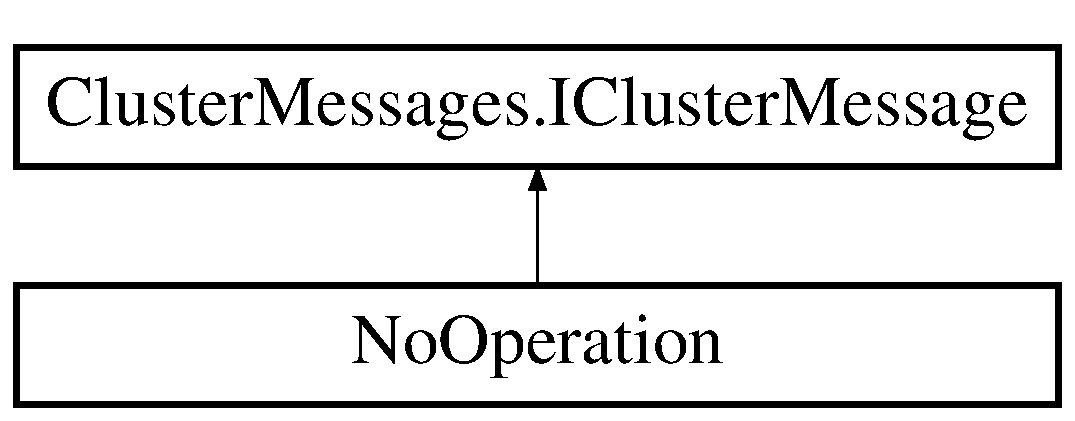
\includegraphics[height=2.000000cm]{class_no_operation}
\end{center}
\end{figure}
\subsection*{Properties}
\begin{DoxyCompactItemize}
\item 
\hypertarget{class_no_operation_a34965a6f307880ac94de6dd23f2ab1b3}{}\hyperlink{class_no_operation_backup_communication_servers}{No\+Operation\+Backup\+Communication\+Servers} \hyperlink{class_no_operation_a34965a6f307880ac94de6dd23f2ab1b3}{Backup\+Communication\+Servers}\hspace{0.3cm}{\ttfamily  \mbox{[}get, set\mbox{]}}\label{class_no_operation_a34965a6f307880ac94de6dd23f2ab1b3}

\begin{DoxyCompactList}\small\item\em $<$uwagi$>$ \end{DoxyCompactList}\end{DoxyCompactItemize}


\subsection{Detailed Description}
$<$uwagi$>$ 

The documentation for this class was generated from the following file\+:\begin{DoxyCompactItemize}
\item 
src/\+Cluster\+Messages/\+Generated\+Messages/No\+Operation.\+cs\end{DoxyCompactItemize}

\hypertarget{class_no_operation_backup_communication_servers}{}\section{No\+Operation\+Backup\+Communication\+Servers Class Reference}
\label{class_no_operation_backup_communication_servers}\index{No\+Operation\+Backup\+Communication\+Servers@{No\+Operation\+Backup\+Communication\+Servers}}


$<$uwagi$>$  


\subsection*{Properties}
\begin{DoxyCompactItemize}
\item 
\hypertarget{class_no_operation_backup_communication_servers_a0a8a0a4824600de87cc8f1b71aef0843}{}\hyperlink{class_no_operation_backup_communication_servers_backup_communication_server}{No\+Operation\+Backup\+Communication\+Servers\+Backup\+Communication\+Server} \hyperlink{class_no_operation_backup_communication_servers_a0a8a0a4824600de87cc8f1b71aef0843}{Backup\+Communication\+Server}\hspace{0.3cm}{\ttfamily  \mbox{[}get, set\mbox{]}}\label{class_no_operation_backup_communication_servers_a0a8a0a4824600de87cc8f1b71aef0843}

\begin{DoxyCompactList}\small\item\em $<$uwagi$>$ \end{DoxyCompactList}\end{DoxyCompactItemize}


\subsection{Detailed Description}
$<$uwagi$>$ 

The documentation for this class was generated from the following file\+:\begin{DoxyCompactItemize}
\item 
src/\+Cluster\+Messages/\+Generated\+Messages/No\+Operation.\+cs\end{DoxyCompactItemize}

\hypertarget{class_no_operation_backup_communication_servers_backup_communication_server}{}\section{No\+Operation\+Backup\+Communication\+Servers\+Backup\+Communication\+Server Class Reference}
\label{class_no_operation_backup_communication_servers_backup_communication_server}\index{No\+Operation\+Backup\+Communication\+Servers\+Backup\+Communication\+Server@{No\+Operation\+Backup\+Communication\+Servers\+Backup\+Communication\+Server}}


$<$uwagi$>$  


\subsection*{Properties}
\begin{DoxyCompactItemize}
\item 
\hypertarget{class_no_operation_backup_communication_servers_backup_communication_server_ae629091935c0deff83ce3b1c7e6c23d3}{}string \hyperlink{class_no_operation_backup_communication_servers_backup_communication_server_ae629091935c0deff83ce3b1c7e6c23d3}{address}\hspace{0.3cm}{\ttfamily  \mbox{[}get, set\mbox{]}}\label{class_no_operation_backup_communication_servers_backup_communication_server_ae629091935c0deff83ce3b1c7e6c23d3}

\begin{DoxyCompactList}\small\item\em $<$uwagi$>$ \end{DoxyCompactList}\item 
\hypertarget{class_no_operation_backup_communication_servers_backup_communication_server_a941b34aabf70f244e5e24ab8057b3e60}{}ushort \hyperlink{class_no_operation_backup_communication_servers_backup_communication_server_a941b34aabf70f244e5e24ab8057b3e60}{port}\hspace{0.3cm}{\ttfamily  \mbox{[}get, set\mbox{]}}\label{class_no_operation_backup_communication_servers_backup_communication_server_a941b34aabf70f244e5e24ab8057b3e60}

\begin{DoxyCompactList}\small\item\em $<$uwagi$>$ \end{DoxyCompactList}\item 
\hypertarget{class_no_operation_backup_communication_servers_backup_communication_server_ac86c2d1d814e601ce170bdddb9ecb63d}{}bool \hyperlink{class_no_operation_backup_communication_servers_backup_communication_server_ac86c2d1d814e601ce170bdddb9ecb63d}{port\+Specified}\hspace{0.3cm}{\ttfamily  \mbox{[}get, set\mbox{]}}\label{class_no_operation_backup_communication_servers_backup_communication_server_ac86c2d1d814e601ce170bdddb9ecb63d}

\begin{DoxyCompactList}\small\item\em $<$uwagi$>$ \end{DoxyCompactList}\end{DoxyCompactItemize}


\subsection{Detailed Description}
$<$uwagi$>$ 

The documentation for this class was generated from the following file\+:\begin{DoxyCompactItemize}
\item 
src/\+Cluster\+Messages/\+Generated\+Messages/No\+Operation.\+cs\end{DoxyCompactItemize}

\hypertarget{class_register}{}\section{Register Class Reference}
\label{class_register}\index{Register@{Register}}


$<$uwagi$>$  


Inheritance diagram for Register\+:\begin{figure}[H]
\begin{center}
\leavevmode
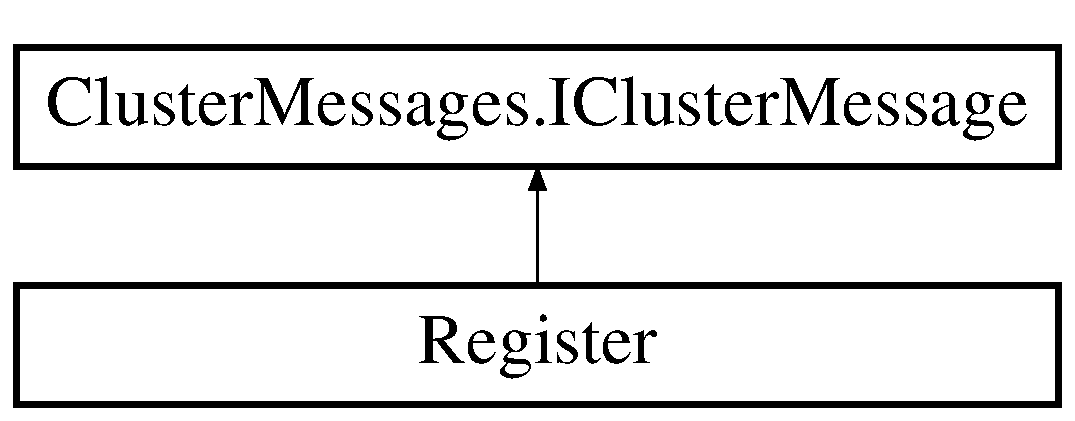
\includegraphics[height=2.000000cm]{class_register}
\end{center}
\end{figure}
\subsection*{Properties}
\begin{DoxyCompactItemize}
\item 
\hypertarget{class_register_a2a79058af7004aa0265253d62b9110f9}{}string \hyperlink{class_register_a2a79058af7004aa0265253d62b9110f9}{Type}\hspace{0.3cm}{\ttfamily  \mbox{[}get, set\mbox{]}}\label{class_register_a2a79058af7004aa0265253d62b9110f9}

\begin{DoxyCompactList}\small\item\em $<$uwagi$>$ \end{DoxyCompactList}\item 
\hypertarget{class_register_a7e055336595d4abe1ab819ad3d2e48fa}{}string \hyperlink{class_register_a7e055336595d4abe1ab819ad3d2e48fa}{Parallel\+Threads}\hspace{0.3cm}{\ttfamily  \mbox{[}get, set\mbox{]}}\label{class_register_a7e055336595d4abe1ab819ad3d2e48fa}

\begin{DoxyCompactList}\small\item\em $<$uwagi$>$ \end{DoxyCompactList}\item 
\hypertarget{class_register_aab81b110159cd4e74dbd25f4bf81167c}{}string \hyperlink{class_register_aab81b110159cd4e74dbd25f4bf81167c}{Deregister}\hspace{0.3cm}{\ttfamily  \mbox{[}get, set\mbox{]}}\label{class_register_aab81b110159cd4e74dbd25f4bf81167c}

\begin{DoxyCompactList}\small\item\em $<$uwagi$>$ \end{DoxyCompactList}\item 
\hypertarget{class_register_ae0bd98b9a644f6067f33a158cabebb17}{}string \hyperlink{class_register_ae0bd98b9a644f6067f33a158cabebb17}{Id}\hspace{0.3cm}{\ttfamily  \mbox{[}get, set\mbox{]}}\label{class_register_ae0bd98b9a644f6067f33a158cabebb17}

\begin{DoxyCompactList}\small\item\em $<$uwagi$>$ \end{DoxyCompactList}\item 
\hypertarget{class_register_a1edb9916b037555931ed163af0beea94}{}\hyperlink{class_register_solvable_problems_problem_name}{Register\+Solvable\+Problems\+Problem\+Name}\mbox{[}$\,$\mbox{]} \hyperlink{class_register_a1edb9916b037555931ed163af0beea94}{Solvable\+Problems}\hspace{0.3cm}{\ttfamily  \mbox{[}get, set\mbox{]}}\label{class_register_a1edb9916b037555931ed163af0beea94}

\begin{DoxyCompactList}\small\item\em $<$uwagi$>$ \end{DoxyCompactList}\end{DoxyCompactItemize}


\subsection{Detailed Description}
$<$uwagi$>$ 

The documentation for this class was generated from the following file\+:\begin{DoxyCompactItemize}
\item 
src/\+Cluster\+Messages/\+Generated\+Messages/Register.\+cs\end{DoxyCompactItemize}

\hypertarget{class_cluster_utils_1_1_registered_component}{}\section{Cluster\+Utils.\+Registered\+Component Class Reference}
\label{class_cluster_utils_1_1_registered_component}\index{Cluster\+Utils.\+Registered\+Component@{Cluster\+Utils.\+Registered\+Component}}


General class for all components that register to main server\+:  


Inheritance diagram for Cluster\+Utils.\+Registered\+Component\+:\begin{figure}[H]
\begin{center}
\leavevmode
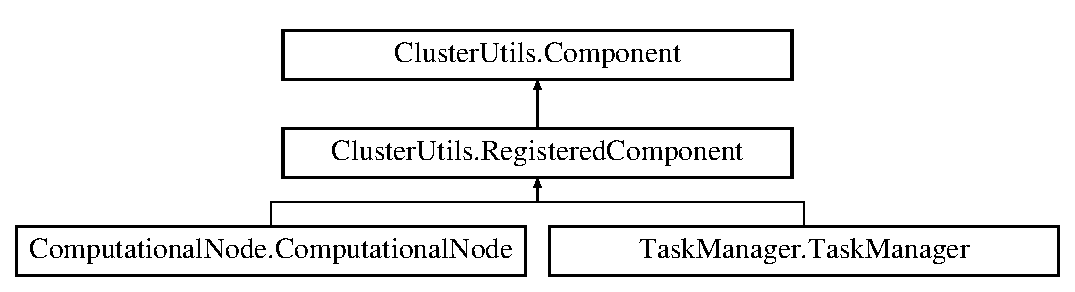
\includegraphics[height=3.000000cm]{class_cluster_utils_1_1_registered_component}
\end{center}
\end{figure}
\subsection*{Public Member Functions}
\begin{DoxyCompactItemize}
\item 
void \hyperlink{class_cluster_utils_1_1_registered_component_a23c088583fe9393f1aed7b4cbf83b449}{Keep\+Sending\+Status} (\hyperlink{class_status}{Status} message, int ms\+Cycle\+Time)
\begin{DoxyCompactList}\small\item\em Method initializing status message timer. \end{DoxyCompactList}\end{DoxyCompactItemize}
\subsection*{Protected Member Functions}
\begin{DoxyCompactItemize}
\item 
\hyperlink{class_cluster_utils_1_1_registered_component_a83b5d230bde822e0fb192b51ebbd2fbc}{Registered\+Component} (\hyperlink{class_cluster_utils_1_1_component_config}{Component\+Config} config, string type)
\item 
bool \hyperlink{class_cluster_utils_1_1_registered_component_a6d986609962aeed78b9a3d091ea5b61c}{Register} ()
\begin{DoxyCompactList}\small\item\em \hyperlink{class_register}{Register} to server and process register response message. \end{DoxyCompactList}\item 
void \hyperlink{class_cluster_utils_1_1_registered_component_afb37c02d49d01aa9accfe203ba89f468}{Start\+Sending\+Status} ()
\begin{DoxyCompactList}\small\item\em Creates status message and timer for status message sending. \end{DoxyCompactList}\item 
void \hyperlink{class_cluster_utils_1_1_registered_component_a83cc1338969d8a9631d81900fc1ddec2}{Process\+No\+Operation\+Message} (Xml\+Document xml\+Message)
\begin{DoxyCompactList}\small\item\em Method processing \hyperlink{class_no_operation}{No\+Operation} message. Retreives backup info. \end{DoxyCompactList}\item 
void \hyperlink{class_cluster_utils_1_1_registered_component_aa06be104c5cf7315d1a6ace42e1e1fc8}{Send\+Message\+No\+Response} (\hyperlink{interface_cluster_messages_1_1_i_cluster_message}{I\+Cluster\+Message} message)
\begin{DoxyCompactList}\small\item\em Helper method for sending message where\textquotesingle{}s no response is expected. \end{DoxyCompactList}\item 
abstract void \hyperlink{class_cluster_utils_1_1_registered_component_ad5ea6fe7d138e7c6bb457c7dca203040}{Process\+Messages} (I\+Enumerable$<$ Xml\+Document $>$ responses)
\begin{DoxyCompactList}\small\item\em Method for handling all messages that given components may handle. \end{DoxyCompactList}\end{DoxyCompactItemize}
\subsection*{Protected Attributes}
\begin{DoxyCompactItemize}
\item 
uint \hyperlink{class_cluster_utils_1_1_registered_component_a0d238d34c162300a2aa7a3caf34689eb}{Id}
\begin{DoxyCompactList}\small\item\em Id received from server after registration. \end{DoxyCompactList}\item 
int \hyperlink{class_cluster_utils_1_1_registered_component_ac95b4af9a774f273a235e31215d6e7bc}{Server\+Timeout}
\begin{DoxyCompactList}\small\item\em Timeout received after registration. \hyperlink{class_status}{Status} message is sent at least as frequent as Server\+Timeout. \end{DoxyCompactList}\item 
readonly List$<$ \hyperlink{class_status_thread}{Status\+Thread} $>$ \hyperlink{class_cluster_utils_1_1_registered_component_a19bb76d070f24ca944bab753b1409b03}{Status\+Threads} = new List$<$\hyperlink{class_status_thread}{Status\+Thread}$>$()
\begin{DoxyCompactList}\small\item\em Container for thread statuses. \end{DoxyCompactList}\end{DoxyCompactItemize}


\subsection{Detailed Description}
General class for all components that register to main server\+: 


\begin{DoxyItemize}
\item Node
\item Manager
\item Server as backup Adds support for component registration and sending status message. 
\end{DoxyItemize}

\subsection{Constructor \& Destructor Documentation}
\hypertarget{class_cluster_utils_1_1_registered_component_a83b5d230bde822e0fb192b51ebbd2fbc}{}\index{Cluster\+Utils\+::\+Registered\+Component@{Cluster\+Utils\+::\+Registered\+Component}!Registered\+Component@{Registered\+Component}}
\index{Registered\+Component@{Registered\+Component}!Cluster\+Utils\+::\+Registered\+Component@{Cluster\+Utils\+::\+Registered\+Component}}
\subsubsection[{Registered\+Component}]{\setlength{\rightskip}{0pt plus 5cm}Cluster\+Utils.\+Registered\+Component.\+Registered\+Component (
\begin{DoxyParamCaption}
\item[{{\bf Component\+Config}}]{config, }
\item[{string}]{type}
\end{DoxyParamCaption}
)\hspace{0.3cm}{\ttfamily [protected]}}\label{class_cluster_utils_1_1_registered_component_a83b5d230bde822e0fb192b51ebbd2fbc}





\begin{DoxyParams}{Parameters}
{\em config} & Server address and port.\\
\hline
{\em type} & \hyperlink{class_cluster_utils_1_1_component}{Component} type.\\
\hline
\end{DoxyParams}


\subsection{Member Function Documentation}
\hypertarget{class_cluster_utils_1_1_registered_component_a23c088583fe9393f1aed7b4cbf83b449}{}\index{Cluster\+Utils\+::\+Registered\+Component@{Cluster\+Utils\+::\+Registered\+Component}!Keep\+Sending\+Status@{Keep\+Sending\+Status}}
\index{Keep\+Sending\+Status@{Keep\+Sending\+Status}!Cluster\+Utils\+::\+Registered\+Component@{Cluster\+Utils\+::\+Registered\+Component}}
\subsubsection[{Keep\+Sending\+Status}]{\setlength{\rightskip}{0pt plus 5cm}void Cluster\+Utils.\+Registered\+Component.\+Keep\+Sending\+Status (
\begin{DoxyParamCaption}
\item[{{\bf Status}}]{message, }
\item[{int}]{ms\+Cycle\+Time}
\end{DoxyParamCaption}
)}\label{class_cluster_utils_1_1_registered_component_a23c088583fe9393f1aed7b4cbf83b449}


Method initializing status message timer. 


\begin{DoxyParams}{Parameters}
{\em message} & Message to be sent.\\
\hline
{\em ms\+Cycle\+Time} & Sending loop time in miliseconds.\\
\hline
\end{DoxyParams}
\hypertarget{class_cluster_utils_1_1_registered_component_ad5ea6fe7d138e7c6bb457c7dca203040}{}\index{Cluster\+Utils\+::\+Registered\+Component@{Cluster\+Utils\+::\+Registered\+Component}!Process\+Messages@{Process\+Messages}}
\index{Process\+Messages@{Process\+Messages}!Cluster\+Utils\+::\+Registered\+Component@{Cluster\+Utils\+::\+Registered\+Component}}
\subsubsection[{Process\+Messages}]{\setlength{\rightskip}{0pt plus 5cm}abstract void Cluster\+Utils.\+Registered\+Component.\+Process\+Messages (
\begin{DoxyParamCaption}
\item[{I\+Enumerable$<$ Xml\+Document $>$}]{responses}
\end{DoxyParamCaption}
)\hspace{0.3cm}{\ttfamily [protected]}, {\ttfamily [pure virtual]}}\label{class_cluster_utils_1_1_registered_component_ad5ea6fe7d138e7c6bb457c7dca203040}


Method for handling all messages that given components may handle. 


\begin{DoxyParams}{Parameters}
{\em responses} & Messages received from server.\\
\hline
\end{DoxyParams}


Implemented in \hyperlink{class_task_manager_1_1_task_manager_aaf525b63d8bb2d1a91ae794ebd016e5b}{Task\+Manager.\+Task\+Manager}, and \hyperlink{class_computational_node_1_1_computational_node_ae7e1583dbbdcdc24d4b342657c4e2d5e}{Computational\+Node.\+Computational\+Node}.

\hypertarget{class_cluster_utils_1_1_registered_component_a83cc1338969d8a9631d81900fc1ddec2}{}\index{Cluster\+Utils\+::\+Registered\+Component@{Cluster\+Utils\+::\+Registered\+Component}!Process\+No\+Operation\+Message@{Process\+No\+Operation\+Message}}
\index{Process\+No\+Operation\+Message@{Process\+No\+Operation\+Message}!Cluster\+Utils\+::\+Registered\+Component@{Cluster\+Utils\+::\+Registered\+Component}}
\subsubsection[{Process\+No\+Operation\+Message}]{\setlength{\rightskip}{0pt plus 5cm}void Cluster\+Utils.\+Registered\+Component.\+Process\+No\+Operation\+Message (
\begin{DoxyParamCaption}
\item[{Xml\+Document}]{xml\+Message}
\end{DoxyParamCaption}
)\hspace{0.3cm}{\ttfamily [protected]}}\label{class_cluster_utils_1_1_registered_component_a83cc1338969d8a9631d81900fc1ddec2}


Method processing \hyperlink{class_no_operation}{No\+Operation} message. Retreives backup info. 


\begin{DoxyParams}{Parameters}
{\em xml\+Message} & Received \hyperlink{class_no_operation}{No\+Operation} message.\\
\hline
\end{DoxyParams}
\hypertarget{class_cluster_utils_1_1_registered_component_a6d986609962aeed78b9a3d091ea5b61c}{}\index{Cluster\+Utils\+::\+Registered\+Component@{Cluster\+Utils\+::\+Registered\+Component}!Register@{Register}}
\index{Register@{Register}!Cluster\+Utils\+::\+Registered\+Component@{Cluster\+Utils\+::\+Registered\+Component}}
\subsubsection[{Register}]{\setlength{\rightskip}{0pt plus 5cm}bool Cluster\+Utils.\+Registered\+Component.\+Register (
\begin{DoxyParamCaption}
{}
\end{DoxyParamCaption}
)\hspace{0.3cm}{\ttfamily [protected]}}\label{class_cluster_utils_1_1_registered_component_a6d986609962aeed78b9a3d091ea5b61c}


\hyperlink{class_register}{Register} to server and process register response message. 

\begin{DoxyReturn}{Returns}
True on registration success, false otherwise.
\end{DoxyReturn}
\hypertarget{class_cluster_utils_1_1_registered_component_aa06be104c5cf7315d1a6ace42e1e1fc8}{}\index{Cluster\+Utils\+::\+Registered\+Component@{Cluster\+Utils\+::\+Registered\+Component}!Send\+Message\+No\+Response@{Send\+Message\+No\+Response}}
\index{Send\+Message\+No\+Response@{Send\+Message\+No\+Response}!Cluster\+Utils\+::\+Registered\+Component@{Cluster\+Utils\+::\+Registered\+Component}}
\subsubsection[{Send\+Message\+No\+Response}]{\setlength{\rightskip}{0pt plus 5cm}void Cluster\+Utils.\+Registered\+Component.\+Send\+Message\+No\+Response (
\begin{DoxyParamCaption}
\item[{{\bf I\+Cluster\+Message}}]{message}
\end{DoxyParamCaption}
)\hspace{0.3cm}{\ttfamily [protected]}}\label{class_cluster_utils_1_1_registered_component_aa06be104c5cf7315d1a6ace42e1e1fc8}


Helper method for sending message where\textquotesingle{}s no response is expected. 


\begin{DoxyParams}{Parameters}
{\em message} & Message to be sent.\\
\hline
\end{DoxyParams}
\hypertarget{class_cluster_utils_1_1_registered_component_afb37c02d49d01aa9accfe203ba89f468}{}\index{Cluster\+Utils\+::\+Registered\+Component@{Cluster\+Utils\+::\+Registered\+Component}!Start\+Sending\+Status@{Start\+Sending\+Status}}
\index{Start\+Sending\+Status@{Start\+Sending\+Status}!Cluster\+Utils\+::\+Registered\+Component@{Cluster\+Utils\+::\+Registered\+Component}}
\subsubsection[{Start\+Sending\+Status}]{\setlength{\rightskip}{0pt plus 5cm}void Cluster\+Utils.\+Registered\+Component.\+Start\+Sending\+Status (
\begin{DoxyParamCaption}
{}
\end{DoxyParamCaption}
)\hspace{0.3cm}{\ttfamily [protected]}}\label{class_cluster_utils_1_1_registered_component_afb37c02d49d01aa9accfe203ba89f468}


Creates status message and timer for status message sending. 



\subsection{Member Data Documentation}
\hypertarget{class_cluster_utils_1_1_registered_component_a0d238d34c162300a2aa7a3caf34689eb}{}\index{Cluster\+Utils\+::\+Registered\+Component@{Cluster\+Utils\+::\+Registered\+Component}!Id@{Id}}
\index{Id@{Id}!Cluster\+Utils\+::\+Registered\+Component@{Cluster\+Utils\+::\+Registered\+Component}}
\subsubsection[{Id}]{\setlength{\rightskip}{0pt plus 5cm}uint Cluster\+Utils.\+Registered\+Component.\+Id\hspace{0.3cm}{\ttfamily [protected]}}\label{class_cluster_utils_1_1_registered_component_a0d238d34c162300a2aa7a3caf34689eb}


Id received from server after registration. 

\hypertarget{class_cluster_utils_1_1_registered_component_ac95b4af9a774f273a235e31215d6e7bc}{}\index{Cluster\+Utils\+::\+Registered\+Component@{Cluster\+Utils\+::\+Registered\+Component}!Server\+Timeout@{Server\+Timeout}}
\index{Server\+Timeout@{Server\+Timeout}!Cluster\+Utils\+::\+Registered\+Component@{Cluster\+Utils\+::\+Registered\+Component}}
\subsubsection[{Server\+Timeout}]{\setlength{\rightskip}{0pt plus 5cm}int Cluster\+Utils.\+Registered\+Component.\+Server\+Timeout\hspace{0.3cm}{\ttfamily [protected]}}\label{class_cluster_utils_1_1_registered_component_ac95b4af9a774f273a235e31215d6e7bc}


Timeout received after registration. \hyperlink{class_status}{Status} message is sent at least as frequent as Server\+Timeout. 

\hypertarget{class_cluster_utils_1_1_registered_component_a19bb76d070f24ca944bab753b1409b03}{}\index{Cluster\+Utils\+::\+Registered\+Component@{Cluster\+Utils\+::\+Registered\+Component}!Status\+Threads@{Status\+Threads}}
\index{Status\+Threads@{Status\+Threads}!Cluster\+Utils\+::\+Registered\+Component@{Cluster\+Utils\+::\+Registered\+Component}}
\subsubsection[{Status\+Threads}]{\setlength{\rightskip}{0pt plus 5cm}readonly List$<${\bf Status\+Thread}$>$ Cluster\+Utils.\+Registered\+Component.\+Status\+Threads = new List$<${\bf Status\+Thread}$>$()\hspace{0.3cm}{\ttfamily [protected]}}\label{class_cluster_utils_1_1_registered_component_a19bb76d070f24ca944bab753b1409b03}


Container for thread statuses. 



The documentation for this class was generated from the following file\+:\begin{DoxyCompactItemize}
\item 
src/\+Cluster\+Utils/Registered\+Component.\+cs\end{DoxyCompactItemize}

\hypertarget{class_register_response}{}\section{Register\+Response Class Reference}
\label{class_register_response}\index{Register\+Response@{Register\+Response}}


$<$uwagi$>$  


Inheritance diagram for Register\+Response\+:\begin{figure}[H]
\begin{center}
\leavevmode
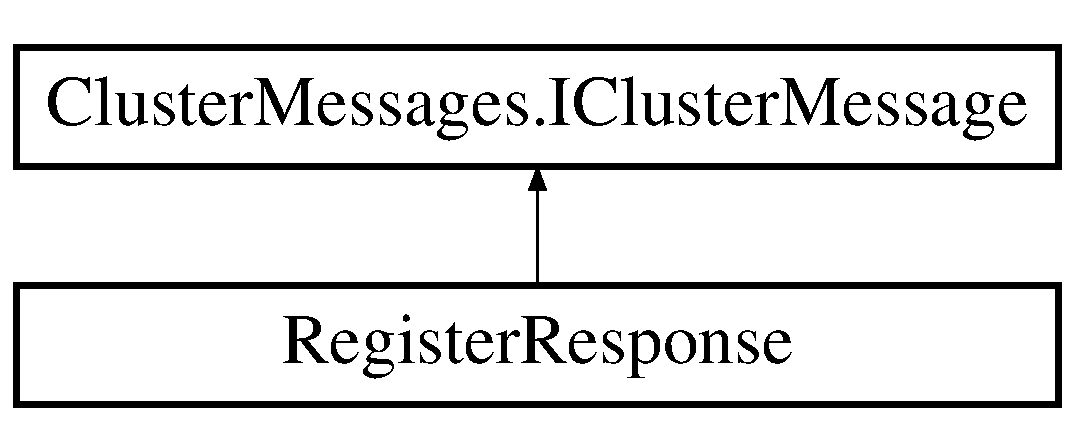
\includegraphics[height=2.000000cm]{class_register_response}
\end{center}
\end{figure}
\subsection*{Properties}
\begin{DoxyCompactItemize}
\item 
\hypertarget{class_register_response_a8a4fdb8d50e4dde3d47365b120073bf5}{}string \hyperlink{class_register_response_a8a4fdb8d50e4dde3d47365b120073bf5}{Id}\hspace{0.3cm}{\ttfamily  \mbox{[}get, set\mbox{]}}\label{class_register_response_a8a4fdb8d50e4dde3d47365b120073bf5}

\begin{DoxyCompactList}\small\item\em $<$uwagi$>$ \end{DoxyCompactList}\item 
\hypertarget{class_register_response_afcae35bb252e654026ceddbdab15cf69}{}string \hyperlink{class_register_response_afcae35bb252e654026ceddbdab15cf69}{Timeout}\hspace{0.3cm}{\ttfamily  \mbox{[}get, set\mbox{]}}\label{class_register_response_afcae35bb252e654026ceddbdab15cf69}

\begin{DoxyCompactList}\small\item\em $<$uwagi$>$ \end{DoxyCompactList}\item 
\hypertarget{class_register_response_ab458693fb9c4b000973ec85adf1d3c60}{}\hyperlink{class_register_response_backup_communication_servers_backup_communication_server}{Register\+Response\+Backup\+Communication\+Servers\+Backup\+Communication\+Server}\mbox{[}$\,$\mbox{]} \hyperlink{class_register_response_ab458693fb9c4b000973ec85adf1d3c60}{Backup\+Communication\+Servers}\hspace{0.3cm}{\ttfamily  \mbox{[}get, set\mbox{]}}\label{class_register_response_ab458693fb9c4b000973ec85adf1d3c60}

\begin{DoxyCompactList}\small\item\em $<$uwagi$>$ \end{DoxyCompactList}\end{DoxyCompactItemize}


\subsection{Detailed Description}
$<$uwagi$>$ 

The documentation for this class was generated from the following file\+:\begin{DoxyCompactItemize}
\item 
src/\+Cluster\+Messages/\+Generated\+Messages/Register\+Response.\+cs\end{DoxyCompactItemize}

\hypertarget{class_register_response_backup_communication_servers_backup_communication_server}{}\section{Register\+Response\+Backup\+Communication\+Servers\+Backup\+Communication\+Server Class Reference}
\label{class_register_response_backup_communication_servers_backup_communication_server}\index{Register\+Response\+Backup\+Communication\+Servers\+Backup\+Communication\+Server@{Register\+Response\+Backup\+Communication\+Servers\+Backup\+Communication\+Server}}


$<$uwagi$>$  


\subsection*{Properties}
\begin{DoxyCompactItemize}
\item 
\hypertarget{class_register_response_backup_communication_servers_backup_communication_server_ac4f62f3709a4ac36811be81903cf8c8f}{}string \hyperlink{class_register_response_backup_communication_servers_backup_communication_server_ac4f62f3709a4ac36811be81903cf8c8f}{address}\hspace{0.3cm}{\ttfamily  \mbox{[}get, set\mbox{]}}\label{class_register_response_backup_communication_servers_backup_communication_server_ac4f62f3709a4ac36811be81903cf8c8f}

\begin{DoxyCompactList}\small\item\em $<$uwagi$>$ \end{DoxyCompactList}\item 
\hypertarget{class_register_response_backup_communication_servers_backup_communication_server_a014d376a0822484d7a472569b0104bb1}{}string \hyperlink{class_register_response_backup_communication_servers_backup_communication_server_a014d376a0822484d7a472569b0104bb1}{port}\hspace{0.3cm}{\ttfamily  \mbox{[}get, set\mbox{]}}\label{class_register_response_backup_communication_servers_backup_communication_server_a014d376a0822484d7a472569b0104bb1}

\begin{DoxyCompactList}\small\item\em $<$uwagi$>$ \end{DoxyCompactList}\end{DoxyCompactItemize}


\subsection{Detailed Description}
$<$uwagi$>$ 

The documentation for this class was generated from the following file\+:\begin{DoxyCompactItemize}
\item 
src/\+Cluster\+Messages/\+Generated\+Messages/Register\+Response.\+cs\end{DoxyCompactItemize}

\hypertarget{class_register_solvable_problems_problem_name}{}\section{Register\+Solvable\+Problems\+Problem\+Name Class Reference}
\label{class_register_solvable_problems_problem_name}\index{Register\+Solvable\+Problems\+Problem\+Name@{Register\+Solvable\+Problems\+Problem\+Name}}


$<$uwagi$>$  


\subsection*{Properties}
\begin{DoxyCompactItemize}
\item 
\hypertarget{class_register_solvable_problems_problem_name_a41d3ac9d91292c1a5632b97ed336fb06}{}string \hyperlink{class_register_solvable_problems_problem_name_a41d3ac9d91292c1a5632b97ed336fb06}{Value}\hspace{0.3cm}{\ttfamily  \mbox{[}get, set\mbox{]}}\label{class_register_solvable_problems_problem_name_a41d3ac9d91292c1a5632b97ed336fb06}

\begin{DoxyCompactList}\small\item\em $<$uwagi$>$ \end{DoxyCompactList}\end{DoxyCompactItemize}


\subsection{Detailed Description}
$<$uwagi$>$ 

The documentation for this class was generated from the following file\+:\begin{DoxyCompactItemize}
\item 
src/\+Cluster\+Messages/\+Generated\+Messages/Register.\+cs\end{DoxyCompactItemize}

\hypertarget{class_communication_server_1_1_server_config}{}\section{Communication\+Server.\+Server\+Config Class Reference}
\label{class_communication_server_1_1_server_config}\index{Communication\+Server.\+Server\+Config@{Communication\+Server.\+Server\+Config}}


Container for server configuration info -\/ listening port, backup/no backup, timeout for components.  


\subsection*{Static Public Member Functions}
\begin{DoxyCompactItemize}
\item 
static \hyperlink{class_communication_server_1_1_server_config}{Server\+Config} \hyperlink{class_communication_server_1_1_server_config_a9dbbd02ff0f943fa1f7dead38726044c}{Load\+From\+App\+Config} ()
\begin{DoxyCompactList}\small\item\em Retreives configuration from App.\+config file. \end{DoxyCompactList}\item 
static \hyperlink{class_communication_server_1_1_server_config}{Server\+Config} \hyperlink{class_communication_server_1_1_server_config_a9f2f4705596c36cc3a07a9ee09a48bcc}{Load\+From\+Arguments} (string\mbox{[}$\,$\mbox{]} arguments)
\begin{DoxyCompactList}\small\item\em Retreives configuration from command line arguments. \end{DoxyCompactList}\item 
static \hyperlink{class_communication_server_1_1_server_config}{Server\+Config} \hyperlink{class_communication_server_1_1_server_config_adfbc64c9c40c2d78db84dd4a02d759fc}{Get\+Server\+Config} (string\mbox{[}$\,$\mbox{]} arguments)
\begin{DoxyCompactList}\small\item\em Retreives config from both App.\+config and command line. Command line arguments supress App.\+config settings. \end{DoxyCompactList}\end{DoxyCompactItemize}
\subsection*{Properties}
\begin{DoxyCompactItemize}
\item 
\hypertarget{class_communication_server_1_1_server_config_a64caffe66540807b6f8cd84c699ba677}{}string {\bfseries Server\+Port}\hspace{0.3cm}{\ttfamily  \mbox{[}get, set\mbox{]}}\label{class_communication_server_1_1_server_config_a64caffe66540807b6f8cd84c699ba677}

\item 
\hypertarget{class_communication_server_1_1_server_config_ac221ca4c04890014733fda564647b03f}{}bool {\bfseries Is\+Backup}\hspace{0.3cm}{\ttfamily  \mbox{[}get, set\mbox{]}}\label{class_communication_server_1_1_server_config_ac221ca4c04890014733fda564647b03f}

\item 
\hypertarget{class_communication_server_1_1_server_config_a9e03b07151cc28c57d8fab75b66d3aeb}{}int {\bfseries Component\+Timeout}\hspace{0.3cm}{\ttfamily  \mbox{[}get, set\mbox{]}}\label{class_communication_server_1_1_server_config_a9e03b07151cc28c57d8fab75b66d3aeb}

\end{DoxyCompactItemize}


\subsection{Detailed Description}
Container for server configuration info -\/ listening port, backup/no backup, timeout for components. 



\subsection{Member Function Documentation}
\hypertarget{class_communication_server_1_1_server_config_adfbc64c9c40c2d78db84dd4a02d759fc}{}\index{Communication\+Server\+::\+Server\+Config@{Communication\+Server\+::\+Server\+Config}!Get\+Server\+Config@{Get\+Server\+Config}}
\index{Get\+Server\+Config@{Get\+Server\+Config}!Communication\+Server\+::\+Server\+Config@{Communication\+Server\+::\+Server\+Config}}
\subsubsection[{Get\+Server\+Config}]{\setlength{\rightskip}{0pt plus 5cm}static {\bf Server\+Config} Communication\+Server.\+Server\+Config.\+Get\+Server\+Config (
\begin{DoxyParamCaption}
\item[{string\mbox{[}$\,$\mbox{]}}]{arguments}
\end{DoxyParamCaption}
)\hspace{0.3cm}{\ttfamily [static]}}\label{class_communication_server_1_1_server_config_adfbc64c9c40c2d78db84dd4a02d759fc}


Retreives config from both App.\+config and command line. Command line arguments supress App.\+config settings. 


\begin{DoxyParams}{Parameters}
{\em arguments} & Command line arguments.\\
\hline
\end{DoxyParams}
\begin{DoxyReturn}{Returns}
Actual server config.
\end{DoxyReturn}
\hypertarget{class_communication_server_1_1_server_config_a9dbbd02ff0f943fa1f7dead38726044c}{}\index{Communication\+Server\+::\+Server\+Config@{Communication\+Server\+::\+Server\+Config}!Load\+From\+App\+Config@{Load\+From\+App\+Config}}
\index{Load\+From\+App\+Config@{Load\+From\+App\+Config}!Communication\+Server\+::\+Server\+Config@{Communication\+Server\+::\+Server\+Config}}
\subsubsection[{Load\+From\+App\+Config}]{\setlength{\rightskip}{0pt plus 5cm}static {\bf Server\+Config} Communication\+Server.\+Server\+Config.\+Load\+From\+App\+Config (
\begin{DoxyParamCaption}
{}
\end{DoxyParamCaption}
)\hspace{0.3cm}{\ttfamily [static]}}\label{class_communication_server_1_1_server_config_a9dbbd02ff0f943fa1f7dead38726044c}


Retreives configuration from App.\+config file. 

\begin{DoxyReturn}{Returns}
Config from App.\+config
\end{DoxyReturn}
\hypertarget{class_communication_server_1_1_server_config_a9f2f4705596c36cc3a07a9ee09a48bcc}{}\index{Communication\+Server\+::\+Server\+Config@{Communication\+Server\+::\+Server\+Config}!Load\+From\+Arguments@{Load\+From\+Arguments}}
\index{Load\+From\+Arguments@{Load\+From\+Arguments}!Communication\+Server\+::\+Server\+Config@{Communication\+Server\+::\+Server\+Config}}
\subsubsection[{Load\+From\+Arguments}]{\setlength{\rightskip}{0pt plus 5cm}static {\bf Server\+Config} Communication\+Server.\+Server\+Config.\+Load\+From\+Arguments (
\begin{DoxyParamCaption}
\item[{string\mbox{[}$\,$\mbox{]}}]{arguments}
\end{DoxyParamCaption}
)\hspace{0.3cm}{\ttfamily [static]}}\label{class_communication_server_1_1_server_config_a9f2f4705596c36cc3a07a9ee09a48bcc}


Retreives configuration from command line arguments. 


\begin{DoxyParams}{Parameters}
{\em arguments} & Command line args.\\
\hline
\end{DoxyParams}
\begin{DoxyReturn}{Returns}
Config from command line args.
\end{DoxyReturn}


The documentation for this class was generated from the following file\+:\begin{DoxyCompactItemize}
\item 
src/\+Communication\+Server/Server\+Config.\+cs\end{DoxyCompactItemize}

\hypertarget{class_communication_server_tests_1_1_server_config_unit_test}{}\section{Communication\+Server\+Tests.\+Server\+Config\+Unit\+Test Class Reference}
\label{class_communication_server_tests_1_1_server_config_unit_test}\index{Communication\+Server\+Tests.\+Server\+Config\+Unit\+Test@{Communication\+Server\+Tests.\+Server\+Config\+Unit\+Test}}
\subsection*{Public Member Functions}
\begin{DoxyCompactItemize}
\item 
\hypertarget{class_communication_server_tests_1_1_server_config_unit_test_a0d61891c3a0cf8b3200a733e361f8de5}{}void {\bfseries Check\+Config\+Availability} ()\label{class_communication_server_tests_1_1_server_config_unit_test_a0d61891c3a0cf8b3200a733e361f8de5}

\item 
\hypertarget{class_communication_server_tests_1_1_server_config_unit_test_a992474a1e65a3d50840c69dce0cbced9}{}void {\bfseries Override\+Server\+Port\+In\+Arguments} ()\label{class_communication_server_tests_1_1_server_config_unit_test_a992474a1e65a3d50840c69dce0cbced9}

\item 
\hypertarget{class_communication_server_tests_1_1_server_config_unit_test_a15a89cd2edcf090ae8aaca6b69e0e021}{}void {\bfseries Override\+Backup\+Status\+In\+Arguments} ()\label{class_communication_server_tests_1_1_server_config_unit_test_a15a89cd2edcf090ae8aaca6b69e0e021}

\item 
\hypertarget{class_communication_server_tests_1_1_server_config_unit_test_a8cd1faa4d847072f60c6028daad542c9}{}void {\bfseries Override\+Timeout\+In\+Arguments} ()\label{class_communication_server_tests_1_1_server_config_unit_test_a8cd1faa4d847072f60c6028daad542c9}

\end{DoxyCompactItemize}


The documentation for this class was generated from the following file\+:\begin{DoxyCompactItemize}
\item 
src/test/\+Communication\+Server\+Tests/Server\+Config\+Unit\+Test.\+cs\end{DoxyCompactItemize}

\hypertarget{class_cluster_utils_1_1_server_info}{}\section{Cluster\+Utils.\+Server\+Info Class Reference}
\label{class_cluster_utils_1_1_server_info}\index{Cluster\+Utils.\+Server\+Info@{Cluster\+Utils.\+Server\+Info}}


Simple container for basic server informations.  


\subsection*{Public Member Functions}
\begin{DoxyCompactItemize}
\item 
\hypertarget{class_cluster_utils_1_1_server_info_a095b6bb7f69811d50212929a82339442}{}{\bfseries Server\+Info} (string port, string address)\label{class_cluster_utils_1_1_server_info_a095b6bb7f69811d50212929a82339442}

\end{DoxyCompactItemize}
\subsection*{Properties}
\begin{DoxyCompactItemize}
\item 
\hypertarget{class_cluster_utils_1_1_server_info_add382573fe9a95890b2ce2c47ffd4d70}{}string {\bfseries Port}\hspace{0.3cm}{\ttfamily  \mbox{[}get, set\mbox{]}}\label{class_cluster_utils_1_1_server_info_add382573fe9a95890b2ce2c47ffd4d70}

\item 
\hypertarget{class_cluster_utils_1_1_server_info_a06bfc80fbfb63af5237dbae97df20dda}{}string {\bfseries Address}\hspace{0.3cm}{\ttfamily  \mbox{[}get, set\mbox{]}}\label{class_cluster_utils_1_1_server_info_a06bfc80fbfb63af5237dbae97df20dda}

\end{DoxyCompactItemize}


\subsection{Detailed Description}
Simple container for basic server informations. 



The documentation for this class was generated from the following file\+:\begin{DoxyCompactItemize}
\item 
src/\+Cluster\+Utils/Server\+Info.\+cs\end{DoxyCompactItemize}

\hypertarget{class_solution_request}{}\section{Solution\+Request Class Reference}
\label{class_solution_request}\index{Solution\+Request@{Solution\+Request}}


$<$uwagi$>$  


Inheritance diagram for Solution\+Request\+:\begin{figure}[H]
\begin{center}
\leavevmode
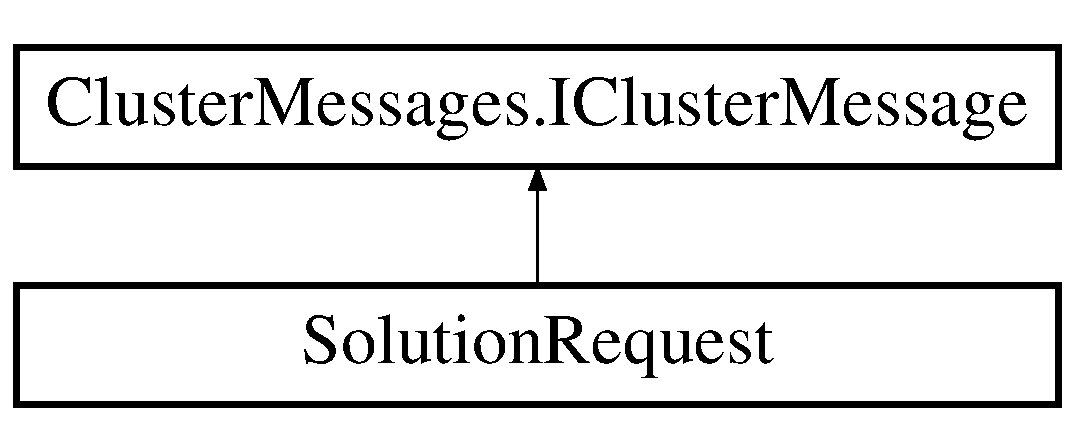
\includegraphics[height=2.000000cm]{class_solution_request}
\end{center}
\end{figure}
\subsection*{Properties}
\begin{DoxyCompactItemize}
\item 
\hypertarget{class_solution_request_a6b1ab40c6b749f684455f79e43d073bf}{}ulong \hyperlink{class_solution_request_a6b1ab40c6b749f684455f79e43d073bf}{Id}\hspace{0.3cm}{\ttfamily  \mbox{[}get, set\mbox{]}}\label{class_solution_request_a6b1ab40c6b749f684455f79e43d073bf}

\begin{DoxyCompactList}\small\item\em $<$uwagi$>$ \end{DoxyCompactList}\end{DoxyCompactItemize}


\subsection{Detailed Description}
$<$uwagi$>$ 

The documentation for this class was generated from the following file\+:\begin{DoxyCompactItemize}
\item 
src/\+Cluster\+Messages/\+Generated\+Messages/Solution\+Request.\+cs\end{DoxyCompactItemize}

\hypertarget{class_solutions}{}\section{Solutions Class Reference}
\label{class_solutions}\index{Solutions@{Solutions}}


$<$uwagi$>$  


Inheritance diagram for Solutions\+:\begin{figure}[H]
\begin{center}
\leavevmode
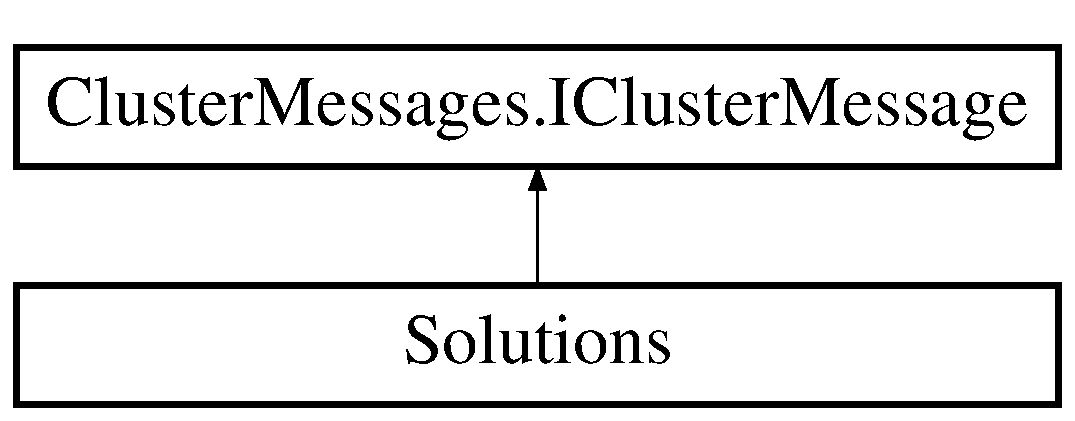
\includegraphics[height=2.000000cm]{class_solutions}
\end{center}
\end{figure}
\subsection*{Properties}
\begin{DoxyCompactItemize}
\item 
\hypertarget{class_solutions_adc5a6394fb6842c6f06931a1faefd882}{}string \hyperlink{class_solutions_adc5a6394fb6842c6f06931a1faefd882}{Problem\+Type}\hspace{0.3cm}{\ttfamily  \mbox{[}get, set\mbox{]}}\label{class_solutions_adc5a6394fb6842c6f06931a1faefd882}

\begin{DoxyCompactList}\small\item\em $<$uwagi$>$ \end{DoxyCompactList}\item 
\hypertarget{class_solutions_ab165186239e40fad38742b9948a0fb72}{}ulong \hyperlink{class_solutions_ab165186239e40fad38742b9948a0fb72}{Id}\hspace{0.3cm}{\ttfamily  \mbox{[}get, set\mbox{]}}\label{class_solutions_ab165186239e40fad38742b9948a0fb72}

\begin{DoxyCompactList}\small\item\em $<$uwagi$>$ \end{DoxyCompactList}\item 
\hypertarget{class_solutions_acd5c1684897098f940fef5173caa58a8}{}byte\mbox{[}$\,$\mbox{]} \hyperlink{class_solutions_acd5c1684897098f940fef5173caa58a8}{Common\+Data}\hspace{0.3cm}{\ttfamily  \mbox{[}get, set\mbox{]}}\label{class_solutions_acd5c1684897098f940fef5173caa58a8}

\begin{DoxyCompactList}\small\item\em $<$uwagi$>$ \end{DoxyCompactList}\item 
\hypertarget{class_solutions_ab51f8e003d60efbf94fa8b7873bc5308}{}\hyperlink{class_solutions_solution}{Solutions\+Solution}\mbox{[}$\,$\mbox{]} \hyperlink{class_solutions_ab51f8e003d60efbf94fa8b7873bc5308}{Solutions1}\hspace{0.3cm}{\ttfamily  \mbox{[}get, set\mbox{]}}\label{class_solutions_ab51f8e003d60efbf94fa8b7873bc5308}

\begin{DoxyCompactList}\small\item\em $<$uwagi$>$ \end{DoxyCompactList}\end{DoxyCompactItemize}


\subsection{Detailed Description}
$<$uwagi$>$ 

The documentation for this class was generated from the following file\+:\begin{DoxyCompactItemize}
\item 
src/\+Cluster\+Messages/\+Generated\+Messages/Solution.\+cs\end{DoxyCompactItemize}

\hypertarget{class_solutions_solution}{}\section{Solutions\+Solution Class Reference}
\label{class_solutions_solution}\index{Solutions\+Solution@{Solutions\+Solution}}


$<$uwagi$>$  


\subsection*{Properties}
\begin{DoxyCompactItemize}
\item 
\hypertarget{class_solutions_solution_a146ffdc6d4b78c7a5505e3f1a6f2ebf6}{}ulong \hyperlink{class_solutions_solution_a146ffdc6d4b78c7a5505e3f1a6f2ebf6}{Task\+Id}\hspace{0.3cm}{\ttfamily  \mbox{[}get, set\mbox{]}}\label{class_solutions_solution_a146ffdc6d4b78c7a5505e3f1a6f2ebf6}

\begin{DoxyCompactList}\small\item\em $<$uwagi$>$ \end{DoxyCompactList}\item 
\hypertarget{class_solutions_solution_a0da9403e39ce1ccb6894ef5783182742}{}bool \hyperlink{class_solutions_solution_a0da9403e39ce1ccb6894ef5783182742}{Task\+Id\+Specified}\hspace{0.3cm}{\ttfamily  \mbox{[}get, set\mbox{]}}\label{class_solutions_solution_a0da9403e39ce1ccb6894ef5783182742}

\begin{DoxyCompactList}\small\item\em $<$uwagi$>$ \end{DoxyCompactList}\item 
\hypertarget{class_solutions_solution_a3731068ae27245c8cc0d994d43ed645c}{}bool \hyperlink{class_solutions_solution_a3731068ae27245c8cc0d994d43ed645c}{Timeout\+Occured}\hspace{0.3cm}{\ttfamily  \mbox{[}get, set\mbox{]}}\label{class_solutions_solution_a3731068ae27245c8cc0d994d43ed645c}

\begin{DoxyCompactList}\small\item\em $<$uwagi$>$ \end{DoxyCompactList}\item 
\hypertarget{class_solutions_solution_a7b9c97daf6483acd817206b1f7a86b7b}{}Solutions\+Solution\+Type \hyperlink{class_solutions_solution_a7b9c97daf6483acd817206b1f7a86b7b}{Type}\hspace{0.3cm}{\ttfamily  \mbox{[}get, set\mbox{]}}\label{class_solutions_solution_a7b9c97daf6483acd817206b1f7a86b7b}

\begin{DoxyCompactList}\small\item\em $<$uwagi$>$ \end{DoxyCompactList}\item 
\hypertarget{class_solutions_solution_ab7b626184f6db4321890256806f75fb5}{}ulong \hyperlink{class_solutions_solution_ab7b626184f6db4321890256806f75fb5}{Computations\+Time}\hspace{0.3cm}{\ttfamily  \mbox{[}get, set\mbox{]}}\label{class_solutions_solution_ab7b626184f6db4321890256806f75fb5}

\begin{DoxyCompactList}\small\item\em $<$uwagi$>$ \end{DoxyCompactList}\item 
\hypertarget{class_solutions_solution_ab6137d1e7ecbff10aea38e1bcfe157c4}{}byte\mbox{[}$\,$\mbox{]} \hyperlink{class_solutions_solution_ab6137d1e7ecbff10aea38e1bcfe157c4}{Data}\hspace{0.3cm}{\ttfamily  \mbox{[}get, set\mbox{]}}\label{class_solutions_solution_ab6137d1e7ecbff10aea38e1bcfe157c4}

\begin{DoxyCompactList}\small\item\em $<$uwagi$>$ \end{DoxyCompactList}\end{DoxyCompactItemize}


\subsection{Detailed Description}
$<$uwagi$>$ 

The documentation for this class was generated from the following file\+:\begin{DoxyCompactItemize}
\item 
src/\+Cluster\+Messages/\+Generated\+Messages/Solution.\+cs\end{DoxyCompactItemize}

\hypertarget{class_solve_partial_problems}{}\section{Solve\+Partial\+Problems Class Reference}
\label{class_solve_partial_problems}\index{Solve\+Partial\+Problems@{Solve\+Partial\+Problems}}


$<$uwagi$>$  


Inheritance diagram for Solve\+Partial\+Problems\+:\begin{figure}[H]
\begin{center}
\leavevmode
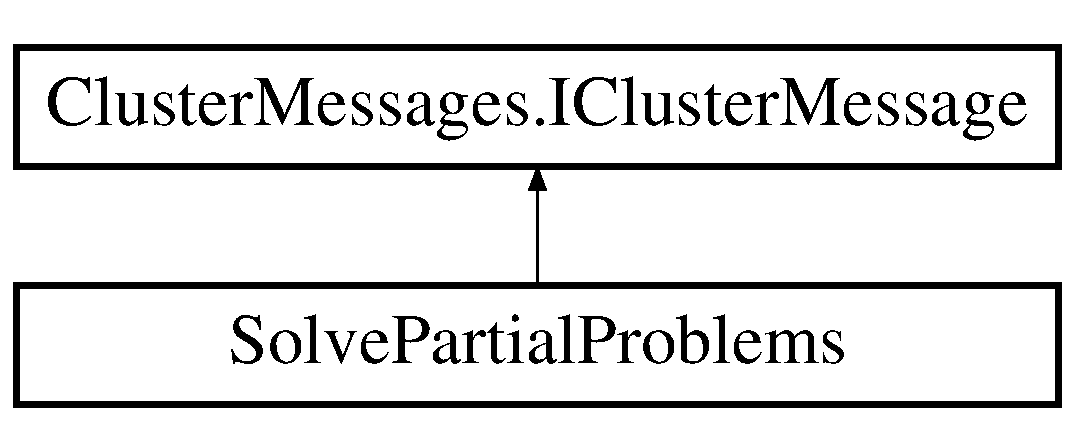
\includegraphics[height=2.000000cm]{class_solve_partial_problems}
\end{center}
\end{figure}
\subsection*{Properties}
\begin{DoxyCompactItemize}
\item 
\hypertarget{class_solve_partial_problems_a5ef9b182e3eeaad8067f41e786050b12}{}string \hyperlink{class_solve_partial_problems_a5ef9b182e3eeaad8067f41e786050b12}{Problem\+Type}\hspace{0.3cm}{\ttfamily  \mbox{[}get, set\mbox{]}}\label{class_solve_partial_problems_a5ef9b182e3eeaad8067f41e786050b12}

\begin{DoxyCompactList}\small\item\em $<$uwagi$>$ \end{DoxyCompactList}\item 
\hypertarget{class_solve_partial_problems_a535bf06a0a0078b807d8c8b4b55030db}{}ulong \hyperlink{class_solve_partial_problems_a535bf06a0a0078b807d8c8b4b55030db}{Id}\hspace{0.3cm}{\ttfamily  \mbox{[}get, set\mbox{]}}\label{class_solve_partial_problems_a535bf06a0a0078b807d8c8b4b55030db}

\begin{DoxyCompactList}\small\item\em $<$uwagi$>$ \end{DoxyCompactList}\item 
\hypertarget{class_solve_partial_problems_aea90359adb9dbb4e4e066e3113e80088}{}byte\mbox{[}$\,$\mbox{]} \hyperlink{class_solve_partial_problems_aea90359adb9dbb4e4e066e3113e80088}{Common\+Data}\hspace{0.3cm}{\ttfamily  \mbox{[}get, set\mbox{]}}\label{class_solve_partial_problems_aea90359adb9dbb4e4e066e3113e80088}

\begin{DoxyCompactList}\small\item\em $<$uwagi$>$ \end{DoxyCompactList}\item 
\hypertarget{class_solve_partial_problems_ae2b161257665b07b9974585de67fa0c2}{}ulong \hyperlink{class_solve_partial_problems_ae2b161257665b07b9974585de67fa0c2}{Solving\+Timeout}\hspace{0.3cm}{\ttfamily  \mbox{[}get, set\mbox{]}}\label{class_solve_partial_problems_ae2b161257665b07b9974585de67fa0c2}

\begin{DoxyCompactList}\small\item\em $<$uwagi$>$ \end{DoxyCompactList}\item 
\hypertarget{class_solve_partial_problems_a863e7cbd5fa8a28e79620cec5455437e}{}bool \hyperlink{class_solve_partial_problems_a863e7cbd5fa8a28e79620cec5455437e}{Solving\+Timeout\+Specified}\hspace{0.3cm}{\ttfamily  \mbox{[}get, set\mbox{]}}\label{class_solve_partial_problems_a863e7cbd5fa8a28e79620cec5455437e}

\begin{DoxyCompactList}\small\item\em $<$uwagi$>$ \end{DoxyCompactList}\item 
\hypertarget{class_solve_partial_problems_a3731e0e9ce8a0aa0f984a16433f2e22c}{}\hyperlink{class_solve_partial_problems_partial_problem}{Solve\+Partial\+Problems\+Partial\+Problem}\mbox{[}$\,$\mbox{]} \hyperlink{class_solve_partial_problems_a3731e0e9ce8a0aa0f984a16433f2e22c}{Partial\+Problems}\hspace{0.3cm}{\ttfamily  \mbox{[}get, set\mbox{]}}\label{class_solve_partial_problems_a3731e0e9ce8a0aa0f984a16433f2e22c}

\begin{DoxyCompactList}\small\item\em $<$uwagi$>$ \end{DoxyCompactList}\end{DoxyCompactItemize}


\subsection{Detailed Description}
$<$uwagi$>$ 

The documentation for this class was generated from the following file\+:\begin{DoxyCompactItemize}
\item 
src/\+Cluster\+Messages/\+Generated\+Messages/Partial\+Problems.\+cs\end{DoxyCompactItemize}

\hypertarget{class_solve_partial_problems_partial_problem}{}\section{Solve\+Partial\+Problems\+Partial\+Problem Class Reference}
\label{class_solve_partial_problems_partial_problem}\index{Solve\+Partial\+Problems\+Partial\+Problem@{Solve\+Partial\+Problems\+Partial\+Problem}}


$<$uwagi$>$  


\subsection*{Properties}
\begin{DoxyCompactItemize}
\item 
\hypertarget{class_solve_partial_problems_partial_problem_ada4c288b3516ef8ec6ad968fecab7962}{}ulong \hyperlink{class_solve_partial_problems_partial_problem_ada4c288b3516ef8ec6ad968fecab7962}{Task\+Id}\hspace{0.3cm}{\ttfamily  \mbox{[}get, set\mbox{]}}\label{class_solve_partial_problems_partial_problem_ada4c288b3516ef8ec6ad968fecab7962}

\begin{DoxyCompactList}\small\item\em $<$uwagi$>$ \end{DoxyCompactList}\item 
\hypertarget{class_solve_partial_problems_partial_problem_ae2b5d38baf6e3b4e36a89a8617a6abfb}{}byte\mbox{[}$\,$\mbox{]} \hyperlink{class_solve_partial_problems_partial_problem_ae2b5d38baf6e3b4e36a89a8617a6abfb}{Data}\hspace{0.3cm}{\ttfamily  \mbox{[}get, set\mbox{]}}\label{class_solve_partial_problems_partial_problem_ae2b5d38baf6e3b4e36a89a8617a6abfb}

\begin{DoxyCompactList}\small\item\em $<$uwagi$>$ \end{DoxyCompactList}\item 
\hypertarget{class_solve_partial_problems_partial_problem_a1a85cea91042baaf387a8372a955cb28}{}ulong \hyperlink{class_solve_partial_problems_partial_problem_a1a85cea91042baaf387a8372a955cb28}{Node\+I\+D}\hspace{0.3cm}{\ttfamily  \mbox{[}get, set\mbox{]}}\label{class_solve_partial_problems_partial_problem_a1a85cea91042baaf387a8372a955cb28}

\begin{DoxyCompactList}\small\item\em $<$uwagi$>$ \end{DoxyCompactList}\end{DoxyCompactItemize}


\subsection{Detailed Description}
$<$uwagi$>$ 

The documentation for this class was generated from the following file\+:\begin{DoxyCompactItemize}
\item 
src/\+Cluster\+Messages/\+Generated\+Messages/Partial\+Problems.\+cs\end{DoxyCompactItemize}

\hypertarget{class_solve_request}{}\section{Solve\+Request Class Reference}
\label{class_solve_request}\index{Solve\+Request@{Solve\+Request}}


$<$uwagi$>$  


Inheritance diagram for Solve\+Request\+:\begin{figure}[H]
\begin{center}
\leavevmode
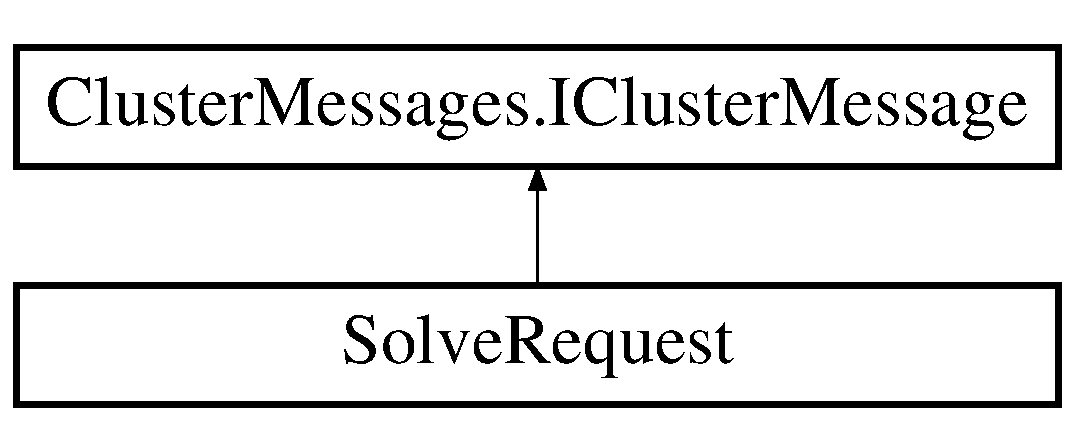
\includegraphics[height=2.000000cm]{class_solve_request}
\end{center}
\end{figure}
\subsection*{Properties}
\begin{DoxyCompactItemize}
\item 
\hypertarget{class_solve_request_a0e67d198115ebb23829fece69edc8bf3}{}string \hyperlink{class_solve_request_a0e67d198115ebb23829fece69edc8bf3}{Problem\+Type}\hspace{0.3cm}{\ttfamily  \mbox{[}get, set\mbox{]}}\label{class_solve_request_a0e67d198115ebb23829fece69edc8bf3}

\begin{DoxyCompactList}\small\item\em $<$uwagi$>$ \end{DoxyCompactList}\item 
\hypertarget{class_solve_request_afdc10407b8a17d2ec2a88f11b21b51d7}{}ulong \hyperlink{class_solve_request_afdc10407b8a17d2ec2a88f11b21b51d7}{Solving\+Timeout}\hspace{0.3cm}{\ttfamily  \mbox{[}get, set\mbox{]}}\label{class_solve_request_afdc10407b8a17d2ec2a88f11b21b51d7}

\begin{DoxyCompactList}\small\item\em $<$uwagi$>$ \end{DoxyCompactList}\item 
\hypertarget{class_solve_request_a773e84a16bff052e68ac75b6ebcb6293}{}bool \hyperlink{class_solve_request_a773e84a16bff052e68ac75b6ebcb6293}{Solving\+Timeout\+Specified}\hspace{0.3cm}{\ttfamily  \mbox{[}get, set\mbox{]}}\label{class_solve_request_a773e84a16bff052e68ac75b6ebcb6293}

\begin{DoxyCompactList}\small\item\em $<$uwagi$>$ \end{DoxyCompactList}\item 
\hypertarget{class_solve_request_aab5d45d2af9c2b57fa7381211679499e}{}byte\mbox{[}$\,$\mbox{]} \hyperlink{class_solve_request_aab5d45d2af9c2b57fa7381211679499e}{Data}\hspace{0.3cm}{\ttfamily  \mbox{[}get, set\mbox{]}}\label{class_solve_request_aab5d45d2af9c2b57fa7381211679499e}

\begin{DoxyCompactList}\small\item\em $<$uwagi$>$ \end{DoxyCompactList}\item 
\hypertarget{class_solve_request_a52636db9a76e39b3688e9a28da7272ea}{}ulong \hyperlink{class_solve_request_a52636db9a76e39b3688e9a28da7272ea}{Id}\hspace{0.3cm}{\ttfamily  \mbox{[}get, set\mbox{]}}\label{class_solve_request_a52636db9a76e39b3688e9a28da7272ea}

\begin{DoxyCompactList}\small\item\em $<$uwagi$>$ \end{DoxyCompactList}\item 
\hypertarget{class_solve_request_ab6cf4376feba6c8ed0b83b28ff99a82e}{}bool \hyperlink{class_solve_request_ab6cf4376feba6c8ed0b83b28ff99a82e}{Id\+Specified}\hspace{0.3cm}{\ttfamily  \mbox{[}get, set\mbox{]}}\label{class_solve_request_ab6cf4376feba6c8ed0b83b28ff99a82e}

\begin{DoxyCompactList}\small\item\em $<$uwagi$>$ \end{DoxyCompactList}\end{DoxyCompactItemize}


\subsection{Detailed Description}
$<$uwagi$>$ 

The documentation for this class was generated from the following file\+:\begin{DoxyCompactItemize}
\item 
src/\+Cluster\+Messages/\+Generated\+Messages/Solve\+Request.\+cs\end{DoxyCompactItemize}

\hypertarget{class_solve_request_response}{}\section{Solve\+Request\+Response Class Reference}
\label{class_solve_request_response}\index{Solve\+Request\+Response@{Solve\+Request\+Response}}


$<$uwagi$>$  


Inheritance diagram for Solve\+Request\+Response\+:\begin{figure}[H]
\begin{center}
\leavevmode
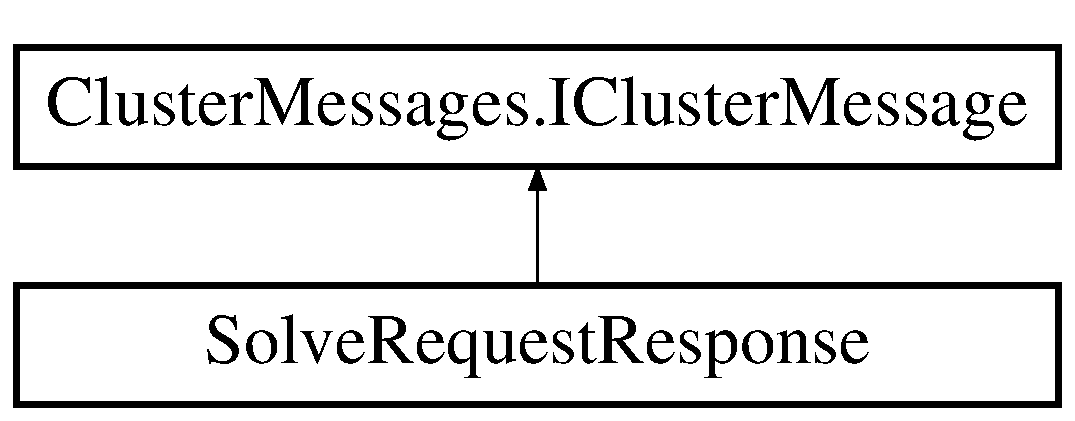
\includegraphics[height=2.000000cm]{class_solve_request_response}
\end{center}
\end{figure}
\subsection*{Properties}
\begin{DoxyCompactItemize}
\item 
\hypertarget{class_solve_request_response_a175bfa0656fa7e0aebe07a645fed5bf9}{}ulong \hyperlink{class_solve_request_response_a175bfa0656fa7e0aebe07a645fed5bf9}{Id}\hspace{0.3cm}{\ttfamily  \mbox{[}get, set\mbox{]}}\label{class_solve_request_response_a175bfa0656fa7e0aebe07a645fed5bf9}

\begin{DoxyCompactList}\small\item\em $<$uwagi$>$ \end{DoxyCompactList}\end{DoxyCompactItemize}


\subsection{Detailed Description}
$<$uwagi$>$ 

The documentation for this class was generated from the following file\+:\begin{DoxyCompactItemize}
\item 
src/\+Cluster\+Messages/\+Generated\+Messages/Solve\+Request\+Response.\+cs\end{DoxyCompactItemize}

\hypertarget{class_cluster_utils_1_1_communication_1_1_state_object}{}\section{Cluster\+Utils.\+Communication.\+State\+Object Class Reference}
\label{class_cluster_utils_1_1_communication_1_1_state_object}\index{Cluster\+Utils.\+Communication.\+State\+Object@{Cluster\+Utils.\+Communication.\+State\+Object}}
\subsection*{Public Attributes}
\begin{DoxyCompactItemize}
\item 
\hypertarget{class_cluster_utils_1_1_communication_1_1_state_object_ac086ce022d558e4f95e12be69130b21a}{}Socket {\bfseries Work\+Socket} = null\label{class_cluster_utils_1_1_communication_1_1_state_object_ac086ce022d558e4f95e12be69130b21a}

\item 
\hypertarget{class_cluster_utils_1_1_communication_1_1_state_object_a5ebc396b146e3456a3517b6fc27cb2e8}{}const int {\bfseries Buffer\+Size} = 1024\label{class_cluster_utils_1_1_communication_1_1_state_object_a5ebc396b146e3456a3517b6fc27cb2e8}

\item 
\hypertarget{class_cluster_utils_1_1_communication_1_1_state_object_a3ac3d5b6d66752e4eef78b3ac14be3bd}{}byte\mbox{[}$\,$\mbox{]} {\bfseries Buffer} = new byte\mbox{[}Buffer\+Size\mbox{]}\label{class_cluster_utils_1_1_communication_1_1_state_object_a3ac3d5b6d66752e4eef78b3ac14be3bd}

\item 
\hypertarget{class_cluster_utils_1_1_communication_1_1_state_object_a6a24d0e1a6df277aa5975c3b7bfd790c}{}List$<$ byte $>$ {\bfseries Byte\+Buffer} = new List$<$byte$>$()\label{class_cluster_utils_1_1_communication_1_1_state_object_a6a24d0e1a6df277aa5975c3b7bfd790c}

\end{DoxyCompactItemize}


The documentation for this class was generated from the following file\+:\begin{DoxyCompactItemize}
\item 
src/\+Cluster\+Utils/\+Communication/State\+Object.\+cs\end{DoxyCompactItemize}

\hypertarget{class_status}{}\section{Status Class Reference}
\label{class_status}\index{Status@{Status}}


$<$uwagi$>$  


Inheritance diagram for Status\+:\begin{figure}[H]
\begin{center}
\leavevmode
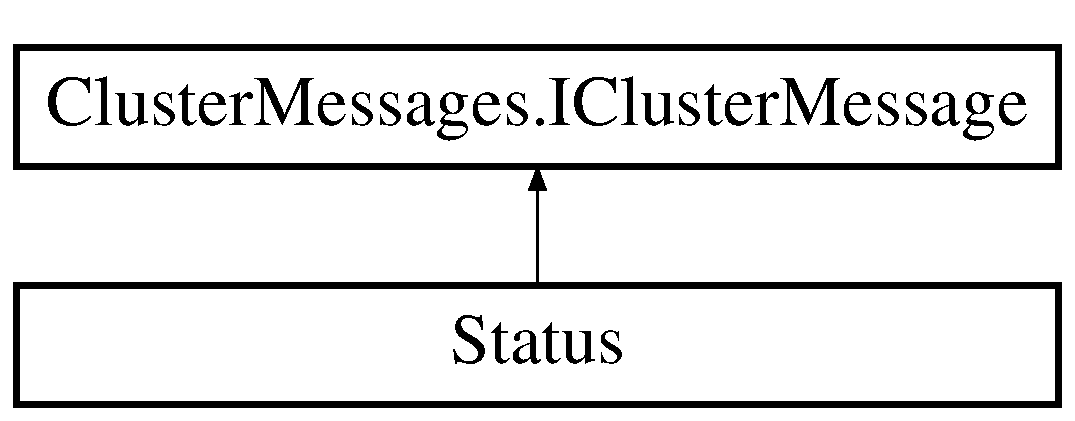
\includegraphics[height=2.000000cm]{class_status}
\end{center}
\end{figure}
\subsection*{Properties}
\begin{DoxyCompactItemize}
\item 
\hypertarget{class_status_a264728427162227f5edf718944bf8a5a}{}ulong \hyperlink{class_status_a264728427162227f5edf718944bf8a5a}{Id}\hspace{0.3cm}{\ttfamily  \mbox{[}get, set\mbox{]}}\label{class_status_a264728427162227f5edf718944bf8a5a}

\begin{DoxyCompactList}\small\item\em $<$uwagi$>$ \end{DoxyCompactList}\item 
\hypertarget{class_status_a9c4063423c7e6840f7f37ed1fdc92672}{}\hyperlink{class_status_thread}{Status\+Thread}\mbox{[}$\,$\mbox{]} \hyperlink{class_status_a9c4063423c7e6840f7f37ed1fdc92672}{Threads}\hspace{0.3cm}{\ttfamily  \mbox{[}get, set\mbox{]}}\label{class_status_a9c4063423c7e6840f7f37ed1fdc92672}

\begin{DoxyCompactList}\small\item\em $<$uwagi$>$ \end{DoxyCompactList}\end{DoxyCompactItemize}


\subsection{Detailed Description}
$<$uwagi$>$ 

The documentation for this class was generated from the following file\+:\begin{DoxyCompactItemize}
\item 
src/\+Cluster\+Messages/\+Generated\+Messages/Status.\+cs\end{DoxyCompactItemize}

\hypertarget{class_status_thread}{}\section{Status\+Thread Class Reference}
\label{class_status_thread}\index{Status\+Thread@{Status\+Thread}}


$<$uwagi$>$  


\subsection*{Properties}
\begin{DoxyCompactItemize}
\item 
\hypertarget{class_status_thread_a73627d278c8db50813754da9cd22b98d}{}Status\+Thread\+State \hyperlink{class_status_thread_a73627d278c8db50813754da9cd22b98d}{State}\hspace{0.3cm}{\ttfamily  \mbox{[}get, set\mbox{]}}\label{class_status_thread_a73627d278c8db50813754da9cd22b98d}

\begin{DoxyCompactList}\small\item\em $<$uwagi$>$ \end{DoxyCompactList}\item 
\hypertarget{class_status_thread_a9b8a8c6e3790c40c173e0237f258d894}{}ulong \hyperlink{class_status_thread_a9b8a8c6e3790c40c173e0237f258d894}{How\+Long}\hspace{0.3cm}{\ttfamily  \mbox{[}get, set\mbox{]}}\label{class_status_thread_a9b8a8c6e3790c40c173e0237f258d894}

\begin{DoxyCompactList}\small\item\em $<$uwagi$>$ \end{DoxyCompactList}\item 
\hypertarget{class_status_thread_a97ddab85d3c9bb59febbfb60a70a6ecb}{}bool \hyperlink{class_status_thread_a97ddab85d3c9bb59febbfb60a70a6ecb}{How\+Long\+Specified}\hspace{0.3cm}{\ttfamily  \mbox{[}get, set\mbox{]}}\label{class_status_thread_a97ddab85d3c9bb59febbfb60a70a6ecb}

\begin{DoxyCompactList}\small\item\em $<$uwagi$>$ \end{DoxyCompactList}\item 
\hypertarget{class_status_thread_abc5cdca139234e3e969980d10705b537}{}ulong \hyperlink{class_status_thread_abc5cdca139234e3e969980d10705b537}{Problem\+Instance\+Id}\hspace{0.3cm}{\ttfamily  \mbox{[}get, set\mbox{]}}\label{class_status_thread_abc5cdca139234e3e969980d10705b537}

\begin{DoxyCompactList}\small\item\em $<$uwagi$>$ \end{DoxyCompactList}\item 
\hypertarget{class_status_thread_a3d90339e0061a5e9becd817ac1b5c2d9}{}bool \hyperlink{class_status_thread_a3d90339e0061a5e9becd817ac1b5c2d9}{Problem\+Instance\+Id\+Specified}\hspace{0.3cm}{\ttfamily  \mbox{[}get, set\mbox{]}}\label{class_status_thread_a3d90339e0061a5e9becd817ac1b5c2d9}

\begin{DoxyCompactList}\small\item\em $<$uwagi$>$ \end{DoxyCompactList}\item 
\hypertarget{class_status_thread_aecb5f93d2e149a63211de8b8339146ee}{}ulong \hyperlink{class_status_thread_aecb5f93d2e149a63211de8b8339146ee}{Task\+Id}\hspace{0.3cm}{\ttfamily  \mbox{[}get, set\mbox{]}}\label{class_status_thread_aecb5f93d2e149a63211de8b8339146ee}

\begin{DoxyCompactList}\small\item\em $<$uwagi$>$ \end{DoxyCompactList}\item 
\hypertarget{class_status_thread_ac7446b65bfa8b7f61eac400762c4abfe}{}bool \hyperlink{class_status_thread_ac7446b65bfa8b7f61eac400762c4abfe}{Task\+Id\+Specified}\hspace{0.3cm}{\ttfamily  \mbox{[}get, set\mbox{]}}\label{class_status_thread_ac7446b65bfa8b7f61eac400762c4abfe}

\begin{DoxyCompactList}\small\item\em $<$uwagi$>$ \end{DoxyCompactList}\item 
\hypertarget{class_status_thread_a178f63000f291d56f8cee191a1a63b5d}{}string \hyperlink{class_status_thread_a178f63000f291d56f8cee191a1a63b5d}{Problem\+Type}\hspace{0.3cm}{\ttfamily  \mbox{[}get, set\mbox{]}}\label{class_status_thread_a178f63000f291d56f8cee191a1a63b5d}

\begin{DoxyCompactList}\small\item\em $<$uwagi$>$ \end{DoxyCompactList}\end{DoxyCompactItemize}


\subsection{Detailed Description}
$<$uwagi$>$ 

The documentation for this class was generated from the following file\+:\begin{DoxyCompactItemize}
\item 
src/\+Cluster\+Messages/\+Generated\+Messages/Status.\+cs\end{DoxyCompactItemize}

\hypertarget{class_task_manager_1_1_task_manager}{}\section{Task\+Manager.\+Task\+Manager Class Reference}
\label{class_task_manager_1_1_task_manager}\index{Task\+Manager.\+Task\+Manager@{Task\+Manager.\+Task\+Manager}}


Implementation of \hyperlink{class_task_manager_1_1_task_manager}{Task\+Manager}. Manager registeres to server and awaits for problems to divide or partial solutions to choose final solution.  


Inheritance diagram for Task\+Manager.\+Task\+Manager\+:\begin{figure}[H]
\begin{center}
\leavevmode
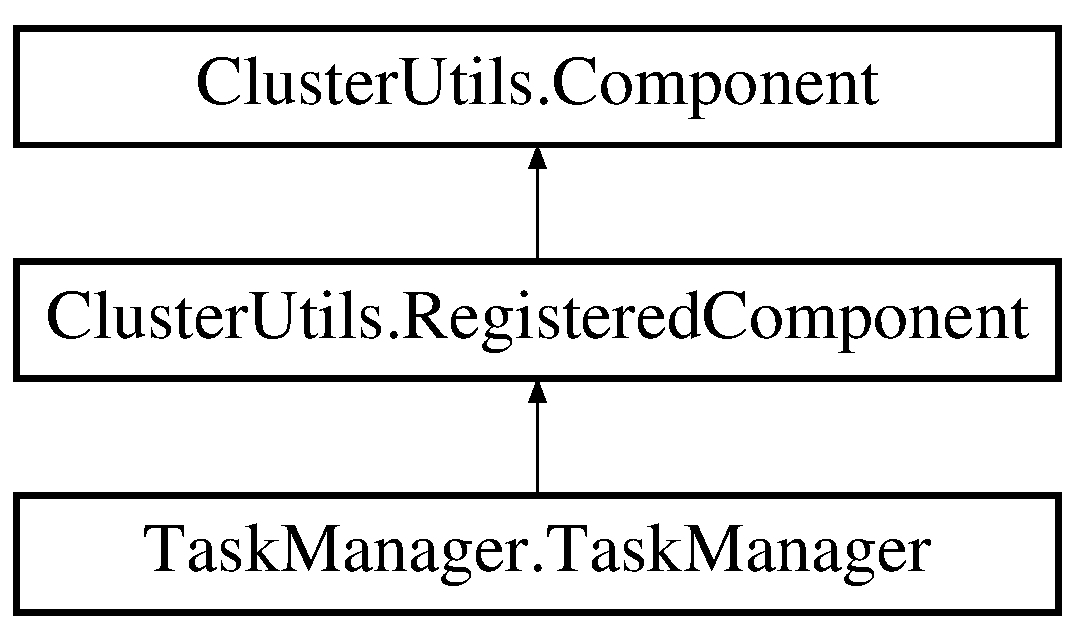
\includegraphics[height=3.000000cm]{class_task_manager_1_1_task_manager}
\end{center}
\end{figure}
\subsection*{Public Member Functions}
\begin{DoxyCompactItemize}
\item 
\hyperlink{class_task_manager_1_1_task_manager_af3c362713451d2f2f38fcf615140daa6}{Task\+Manager} (\hyperlink{class_cluster_utils_1_1_component_config}{Component\+Config} config)
\item 
void \hyperlink{class_task_manager_1_1_task_manager_afd66af2649a0a2e6747258b73853c4aa}{Start} ()
\begin{DoxyCompactList}\small\item\em Tries to register to server and starts sending status message. \end{DoxyCompactList}\end{DoxyCompactItemize}
\subsection*{Protected Member Functions}
\begin{DoxyCompactItemize}
\item 
override void \hyperlink{class_task_manager_1_1_task_manager_aaf525b63d8bb2d1a91ae794ebd016e5b}{Process\+Messages} (I\+Enumerable$<$ Xml\+Document $>$ responses)
\begin{DoxyCompactList}\small\item\em Method for handling all messages that given components may handle. \end{DoxyCompactList}\end{DoxyCompactItemize}
\subsection*{Additional Inherited Members}


\subsection{Detailed Description}
Implementation of \hyperlink{class_task_manager_1_1_task_manager}{Task\+Manager}. Manager registeres to server and awaits for problems to divide or partial solutions to choose final solution. 



\subsection{Constructor \& Destructor Documentation}
\hypertarget{class_task_manager_1_1_task_manager_af3c362713451d2f2f38fcf615140daa6}{}\index{Task\+Manager\+::\+Task\+Manager@{Task\+Manager\+::\+Task\+Manager}!Task\+Manager@{Task\+Manager}}
\index{Task\+Manager@{Task\+Manager}!Task\+Manager\+::\+Task\+Manager@{Task\+Manager\+::\+Task\+Manager}}
\subsubsection[{Task\+Manager}]{\setlength{\rightskip}{0pt plus 5cm}Task\+Manager.\+Task\+Manager.\+Task\+Manager (
\begin{DoxyParamCaption}
\item[{{\bf Component\+Config}}]{config}
\end{DoxyParamCaption}
)}\label{class_task_manager_1_1_task_manager_af3c362713451d2f2f38fcf615140daa6}





\begin{DoxyParams}{Parameters}
{\em config} & Server info from App.\+config and arguments.\\
\hline
\end{DoxyParams}


\subsection{Member Function Documentation}
\hypertarget{class_task_manager_1_1_task_manager_aaf525b63d8bb2d1a91ae794ebd016e5b}{}\index{Task\+Manager\+::\+Task\+Manager@{Task\+Manager\+::\+Task\+Manager}!Process\+Messages@{Process\+Messages}}
\index{Process\+Messages@{Process\+Messages}!Task\+Manager\+::\+Task\+Manager@{Task\+Manager\+::\+Task\+Manager}}
\subsubsection[{Process\+Messages}]{\setlength{\rightskip}{0pt plus 5cm}override void Task\+Manager.\+Task\+Manager.\+Process\+Messages (
\begin{DoxyParamCaption}
\item[{I\+Enumerable$<$ Xml\+Document $>$}]{responses}
\end{DoxyParamCaption}
)\hspace{0.3cm}{\ttfamily [protected]}, {\ttfamily [virtual]}}\label{class_task_manager_1_1_task_manager_aaf525b63d8bb2d1a91ae794ebd016e5b}


Method for handling all messages that given components may handle. 


\begin{DoxyParams}{Parameters}
{\em responses} & Messages received from server.\\
\hline
\end{DoxyParams}


Implements \hyperlink{class_cluster_utils_1_1_registered_component_ad5ea6fe7d138e7c6bb457c7dca203040}{Cluster\+Utils.\+Registered\+Component}.

\hypertarget{class_task_manager_1_1_task_manager_afd66af2649a0a2e6747258b73853c4aa}{}\index{Task\+Manager\+::\+Task\+Manager@{Task\+Manager\+::\+Task\+Manager}!Start@{Start}}
\index{Start@{Start}!Task\+Manager\+::\+Task\+Manager@{Task\+Manager\+::\+Task\+Manager}}
\subsubsection[{Start}]{\setlength{\rightskip}{0pt plus 5cm}void Task\+Manager.\+Task\+Manager.\+Start (
\begin{DoxyParamCaption}
{}
\end{DoxyParamCaption}
)}\label{class_task_manager_1_1_task_manager_afd66af2649a0a2e6747258b73853c4aa}


Tries to register to server and starts sending status message. 



The documentation for this class was generated from the following file\+:\begin{DoxyCompactItemize}
\item 
src/\+Task\+Manager/Task\+Manager.\+cs\end{DoxyCompactItemize}

\hypertarget{class_communication_server_1_1_thread_package}{}\section{Communication\+Server.\+Thread\+Package Class Reference}
\label{class_communication_server_1_1_thread_package}\index{Communication\+Server.\+Thread\+Package@{Communication\+Server.\+Thread\+Package}}
\subsection*{Public Member Functions}
\begin{DoxyCompactItemize}
\item 
\hypertarget{class_communication_server_1_1_thread_package_ae68ad842ce89d51084c298d0aed6b288}{}{\bfseries Thread\+Package} (Socket h, Xml\+Document m)\label{class_communication_server_1_1_thread_package_ae68ad842ce89d51084c298d0aed6b288}

\end{DoxyCompactItemize}
\subsection*{Public Attributes}
\begin{DoxyCompactItemize}
\item 
\hypertarget{class_communication_server_1_1_thread_package_a1b387a120f124b1c941a059c60b42c3e}{}Socket {\bfseries Handler}\label{class_communication_server_1_1_thread_package_a1b387a120f124b1c941a059c60b42c3e}

\item 
\hypertarget{class_communication_server_1_1_thread_package_a3c91800d1765e7148985a6513bda863e}{}Xml\+Document {\bfseries Message}\label{class_communication_server_1_1_thread_package_a3c91800d1765e7148985a6513bda863e}

\end{DoxyCompactItemize}


The documentation for this class was generated from the following file\+:\begin{DoxyCompactItemize}
\item 
src/\+Communication\+Server/Thread\+Package.\+cs\end{DoxyCompactItemize}

%--- End generated contents ---

% Index
\backmatter
\newpage
\phantomsection
\clearemptydoublepage
\addcontentsline{toc}{chapter}{Index}
\printindex

\end{document}
